\documentclass{elsarticle}
\usepackage[utf8]{inputenc}

\usepackage{tikz-cd}
\usepackage{subfig}

\usepackage{graphicx}
\usepackage{caption}
\usepackage{xspace}
\usepackage{color}
\usepackage{subfig}
\usepackage{epstopdf}% To incorporate .eps illustrations using PDFLaTeX, etc.
\usepackage{comment}
\newcommand{\stefano}[1]{{\color{red}#1}}
\newcommand{\stefanoDone}[1]{{\color{black}#1}}
\newcommand{\andrea}[1]{{\color{blue}#1}}
\newcommand{\ramy}[1]{{\color{cyan}#1}}
\newcommand{\notshow}[1]{}

%\usepackage[nolists,tablesfirst]{endfloat}% To `separate' figures and tables from text if required
\usepackage{amsmath,amssymb}
\usepackage{dsfont}
\usepackage{bm}
\usepackage{mathrsfs}
\usepackage{amsthm}
\usepackage{a4wide}

\usepackage{multirow}
\usepackage{diffcoeff}
\usepackage{arydshln,mathtools}% http://ctan.org/pkg/{arydshln,leftidx,mathtools}
\usepackage[most]{tcolorbox}


\usepackage[numbers]{natbib}% Citation support using natbib.sty
%\bibpunct[, ]{(}{)}{;}{a}{}{,}% Citation support using natbib.sty
%\renewcommand\bibfont{\fontsize{10}{12}\selectfont}% Bibliography support using natbib.sty
\bibliographystyle{unsrtnat}


\newtheorem{theorem}{Theorem}
\newtheorem{definition}{Definition}
\newtheorem{remark}{Remark}
\newtheorem{proposition}{Proposition}
\newtheorem{formula}{Formula}
\newtheorem{corollary}{Corollary}
\newtheorem{assumption}{Assumption}
\newtheorem{example}{Example}

\renewcommand\d{\ensuremath{\mathrm{d}}}


% inner products
\def\onedot{$\mathsurround0pt\ldotp$}
\def\cddot{% two dots stacked vertically
	\mathbin{\vcenter{\baselineskip.67ex
			\hbox{\onedot}\hbox{\onedot}}%
}}

\newcommand{\bbR}{\mathbb{R}}
\newcommand{\bbF}{\mathbb{F}}
\newcommand{\bbA}{\mathbb{A}}
\newcommand{\bbB}{\mathbb{B}}
\newcommand{\bbS}{\mathbb{S}}

\DeclareMathOperator{\tr}{tr}

\newcommand*{\dual}[1]{\ensuremath{\widehat{#1}}}
\newcommand*{\norm}[1]{\ensuremath{\left\|#1\right\|}}
\newcommand{\where}{\qquad \text{where} \qquad}

\newcommand{\inpr}[3][]{\ensuremath{\langle #2, \, #3 \rangle_{#1}}}

\newcommand{\dualpr}[3][]{\ensuremath{\langle #2 \, \vert #3 \rangle_{#1}}}


\newcommand{\pder}[2]{\ensuremath{\partial_{#2} #1}}
\newcommand{\dder}[2]{\ensuremath{\delta_{#2} #1}}

\DeclareMathOperator*{\grad}{grad}
\DeclareMathOperator*{\Grad}{Grad}
\DeclareMathOperator*{\Div}{Div}
\renewcommand{\div}{\operatorname{div}}
\DeclareMathOperator*{\Hess}{Hess}
\DeclareMathOperator*{\curl}{curl}

\newcommand{\secref}[1]{\S\ref{#1}}
\newcommand{\energy}[1]{\frac{1}{2} \int_{\Omega} \left\{ #1 \right\} \d\Omega}
\newcommand{\crmat}[1]{\ensuremath{\left[#1\right]_\times}}
\newcommand{\fenics}{\textsc{FEniCS}\xspace}
\newcommand{\firedrake}{\textsc{Firedrake}\xspace}


\journal{ArXiv}

\graphicspath{{./images/}}

\begin{document}

\begin{frontmatter}	
		%% Title, authors and addresses
		
		%% use the tnoteref command within \title for footnotes;
		%% use the tnotetext command for theassociated footnote;
		%% use the fnref command within \author or \address for footnotes;
		%% use the fntext command for theassociated footnote;
		%% use the corref command within \author for corresponding author footnotes;
		%% use the cortext command for theassociated footnote;
		%% use the ead command for the email address,
		%% and the form \ead[url] for the home page:
		%% \title{Title\tnoteref{label1}}
		%% \tnotetext[label1]{}
		%% \author{Name\corref{cor1}\fnref{label2}}
		%% \ead{email address}
		%% \ead[url]{home page}
		%% \fntext[label2]{}
		%% \cortext[cor1]{}
		%% \address{Address\fnref{label3}}
		%% \fntext[label3]{}	
		\title{Dual field structure-preserving discretization of port-Hamiltonian systems using finite element exterior calculus}	
		%% use optional labels to link authors explicitly to addresses:
		%% \author[label1,label2]{}
		%% \address[label1]{}
		%% \address[label2]{}
		\author[UT]{Andrea Brugnoli\corref{cor1}}
		\ead{a.brugnoli@utwente.nl}
		
		\cortext[cor1]{Corresponding author}
	    \author[UT]{Ramy Rashad}
	    \ead{r.a.m.rashadhashem@utwente.nl}
        \author[UT]{Stefano Stramigioli}
        \ead{s.stramigioli@utwente.nl}

	    \address[UT]{Robotics and Mechatronics Department, University of Twente, The Netherlands}

		\begin{abstract}
	
	In this paper we propose a novel approach to discretize linear port-Hamiltonian systems while preserving the underlying structure. We present a finite element exterior calculus formulation that is able to mimetically represent conservation laws and cope with mixed open boundary conditions using a single computational mesh.
	The possibility of including open boundary conditions allows for modular composition of complex multi-physical systems whereas the exterior calculus formulation provides a coordinate-free treatment.
	Our approach relies on a dual-field representation of the physical system that is redundant at the continuous level but eliminates the need of mimicking the Hodge star operator at the discrete level.
	By considering the Stokes-Dirac structure representing the system together with its adjoint, which  embeds the metric information directly in the codifferential, the need for an explicit discrete Hodge star is avoided altogether.
	By imposing the boundary conditions in a strong manner, the power balance characterizing the Stokes-Dirac structure is then retrieved at the discrete level via symplectic Runge-Kutta integrators based on Gauss-Legendre collocation points. Numerical experiments validate the convergence of the method and the conservation properties in terms of energy balance both  for the wave and Maxwell equations in a three dimensional domain. For the latter example, the magnetic and electric fields preserve their divergence free nature at the discrete level.

		\end{abstract}
		
		\begin{keyword}
			%% keywords here, in the form: keyword \sep keyword
			%% PACS codes here, in the form: \PACS code \sep code
			%% MSC codes here, in the form: \MSC code \sep code
			%% or \MSC[2008] code \sep code (2000 is the default)
			 Port-Hamiltonian systems \sep Structure preserving discretization \sep Finite element exterior calculus \sep de Rham complex \sep Dual field representation 
		\end{keyword}
	
	
   
	\end{frontmatter}
	
\section{Introduction}

The field of computational engineering seeks to advance the reliability and accuracy of simulations by means of faster and/or higher fidelity algorithms. Complex engineering systems arise from the interconnection of many simple components. For this reason, it is important that computational models be also constructed via a modular approach, where each subsystem is modelled separately and then assembled to the rest (as in dynamic substructuring). Furthermore, even more important is the fact that such models can be reusable and are to a big extent independent of the super-model they will be part of. This idea is at the core of the port-Hamiltonian (pH) framework, since it describes the interaction between systems and the surrounding environment by means of ports (cf. \cite{maschke1993pH} for the first paper discussing pH finite dimensional systems and their connection with bond-graph modelling). In the infinite dimensional case the mathematical literature has been mostly focused on Hamiltonian systems  with no interaction with the environment (see \cite{olver1986applications} for a reference on the subject). However in the seminal work \cite{vanderSchaft2002}, distributed pH systems were first introduced to model physical systems of conservation laws (which happen to be described by hyperbolic PDEs due to the physical finite propagation time). In order to account for the non-trivial boundary interaction, the authors introduced the concept of Stokes-Dirac structure. This geometrical structure represents an extension of Dirac manifolds \cite{courant1990} to the infinite dimensional case. The Stokes theorem allows defining appropriate boundary variables to account for the power exchange through the boundary of the spatial domain. This geometrical structure is acausal, in the sense that it ignores the actual boundary conditions of the problem at hand, and simply captures all admissible boundary flows. \\


Distributed pH systems bring together different areas of mathematics, physics and engineering. They were first formulated using the language of differential geometry but their mathematical as well as system theoretic properties have also being studied in a functional analytic setting (cf.  \cite{legorrec2005,villegas2007port,skrepek2021,birgit2021riesz} for works on mathematical wellposedness and \cite{ramirez2014exponential,augner2014stability} for studies on stability and stabilization). Since they are closed under interconnection (this feature stems from the properties of the Dirac structure \cite{cervera2007int}), pH systems have the potential to tackle complex multiphysical engineering applications.  So far they were employed to model fluid-structure coupled phenomena \cite{cardoso2017}, reactive flows \cite{altmann2017reactive},  Euler and Navier-Stokes equations \cite{rashad2021part1,rashad2021part2,califano2021ns}, thin mechanical and thermomecanical structures \cite{brugnoli2020,brugnoli2021thermo}. The interested reader may consult \cite{rashad2020review} for a comprehensive review on distributed pH systems. \\

To exploit the full potential of this novel modelling framework, discretization schemes must retain the many properties of pH systems. In particular, numerical algorithms should capture the underlying conservation laws and provide a systematic way to handle boundary conditions, so that the resulting discrete pH system defines a (modular) Dirac structure. The first contribution in this sense dates back to \cite{golo2004hamiltonian}. Therein, the Stokes-Dirac structure is discrete in strong form exploiting mixed finite element differential forms and compatibility conditions need to be fulfilled\footnote{These conditions turn out to be very particular cases of the bounded commuting projectors of the Finite Element Exterior calculus framework \cite{arnold2006acta}.}.
A reduction method based on symplectic Gauss-Legendre collocation points is detailed in \cite{moulla2012pseudo}. This methodology suffers a major drawback, as it cannot handle higher dimensional spatial domains. A staggered finite difference strategy is proposed in \cite{trenchant2018} but the scheme is specialized for the wave equation only. The discrete exterior calculus framework \cite{hirani2003discrete}, based on algebraic topology, can also be used to formulate pH systems in a purely discrete manner, as shown in \cite{seslija2014simplicial}. However, this framework does not rely on interpolating basis function but only on  mimetic discrete operators that reproduce the behaviour of their continuous counterparts. This makes necessary the employment of dual topological meshes, based on the Delaunay-Voronoi duality, to construct an isomorphic discrete Hodge star. This limits the applicability of the method, as dual meshes requires ghost points that do not lie inside the physical domain, thus making it difficult to interconnect systems along a physical boundary. In order to avoid the need for dual meshes, a Galerkin formulation based on Whitney forms is detailed in \cite{kotyczka2019discrete}. In order to construct a minimal bond space, projector matrices parametrized by tunable parameters need to be introduced. The best choice of these parameters depends strongly on the application at hand and this complicates the employment of the method. When only one computational mesh is used, it is not possible to construct a discrete isomorphic Hodge operator \cite{hiptmair2001,bochev2006}. The resulting discrete is merely a projector for dual finite element spaces and therefore it introduces an additional discretization error. However, mixed finite elements do not rely on a discrete Hodge, but rather on a weak formulation of the codifferential operator via the integration by parts formula. This was formalized by the Partitioned Finite Element method \cite{cardoso2020pfem}. \\

From the past literature, it may look like new tools and implementations are needed to be able to capture the particular features of pH systems. In this paper we argue the opposite. The pH modelling paradigm represent a unifying framework to describe physical problems. As such, it should be discretized via a unifying discretization method: the Finite Element Exterior calculus theory  \cite{arnold2006acta} provides all the tools needed to accomplish this task. Using finite element differential forms, a discrete counterpart of the Stokes-Dirac structure can be easily obtained. However, the discretization of constitutive equations remain problematic as those require a discrete Hodge star. Recently, a dual field formulation has been introduced to discretize the Navier-Stokes \cite{zhang2021mass}. This methodology seeks variables in dual polynomial finite element spaces via a mixed finite element formulation and is capable of conserving mass, helicity and energy. A staggered time discretization, in which the vorticity information is exchanged between the two systems, allows treating the non linear rotational term in a linear fashion and makes this scheme computationally competitive with state of the art method. 
This method has a clear connection with Hamiltonian dynamical systems, as discussed by the authors in the introduction of the paper. Furthermore, it relies on the Finite Element Exterior calculus framework as the finite element used therein (the so-called mimetic quadrilateral/hexahedral finite elements \cite{palha2014mimetic}) form a discrete de Rham complex. \\

In this contribution, we show how the dual field formulation can be used for the systematic discretization of linear pH systems (but the framework is extendable to the state modulated case where one has a Poisson manifold, as already done in \cite{zhang2021mass}). To show the generality of the approach, we detail the calculations in exterior calculus. The dual field formulation is based on the construction of an adjoint Stokes-Dirac structure, where the flows and efforts are the Hodge dual of the initial Stokes-Dirac structure. The introduction of an adjoint system leads to a redundant representation of the dynamics, as the state variables are doubled. Nevertheless, this redundancy removes the need for a discrete Hodge star, as one can use dual variables to expresses the energy as a duality product of forms, rather than the classical inner product. The Stokes-Dirac structure can be immediately discretized in a mimetic fashion, whereas the adjoint Stokes-Dirac structure requires the integration by part formula to obtain a discrete representation of the codifferential. The constitutive equations are embedded in the dynamics by expressing the state variables in terms of the effort ones. In other words, by using a redundant dual system, the state variables will be the original ones, plus the Hodge star of the former. In this way, it is possible to calculate the needed efforts corresponding to the differential of the energy function, without any need of the Hodge operation. The boundary conditions are here imposed strongly. This choice leads to two uncoupled mixed finite element discretization of the dynamical pH systems, each containing two unknowns (as in the Partitioned Finite Element method).  In this way, after these two systems are integrated on the same time grid via symplectic collocation Runge-Kutta methods (for simplicity the implicit midpoint scheme will be used here), an exact discrete power balance is retrieved. This implies that the discretization scheme gives rise to a Dirac structure and can be used for interconnecting different physical systems in a structured fashion. We detail the discrete operations (like the inner and duality products, the exterior derivative and the trace) using the trimmed polynomial spaces. The lowest order case coincide with the Whitney forms \cite{whitney1957}. The Whitney forms are particularly meaningful, since they make explicit a number of concepts  like metrical versus topological properties and operations. Numerical tests, assessing the conservation properties of the scheme and the convergence rate of the different variables, are performed on the wave and Maxwell equations in a three dimensional Euclidean domain\footnote{The implementation of the finite element method on a triangulated polyhedral manifold is immediate when the manifold is embedded in Euclidean space \cite{arnold2018finite}.}. Since each of the two mixed discretisation converges to the exact solution under mesh refinement, this redundant representation does not exhibit synchronisation problems and provides a dual finite element representation of the underlying exact solution. The well established open-source library \firedrake \cite{rathgeber2017firedrake} is employed for the implementation (but one can also use the \fenics \cite{logg2012} library). \\

The paper is organised as follows: in Sec. \ref{sec:prel} some preliminaries on needed concepts and notation will be presented. In Sec. \ref{sec:pradj_SDS} we introduce the concept and representation of the primal and adjoint Stokes-Dirac structure and the associated pH systems which is instrumental in the presented solution. The weak formulation, upon which the discretization scheme is based, is presented in Sec. \ref{sec:weak_df}. The spatial discretization is illustrated in Sec. \ref{sec:space_discr} by means of the trimmed polynomial spaces. We detail the discrete version of the dual field Stokes-Dirac structure as well as the associated dynamical system. In Sec. \ref{sec:time_discr}, the time discretization is explained using the implicit midpoint method. Sec. \ref{sec:num_exp} collects the numerical tests and shows the numerical performances of the proposed methodology. 

\section{Preliminaries}\label{sec:prel}
In this section we will introduce some preliminary concepts and their notation which are needed for the treatment ahead. In particular, we will introduce materials from algebraic topology, exterior calculus and finite element differential forms. The presented material is inspired by \cite{bochev2006,arnold2018finite}.

\subsection{Algebraic topology}



\begin{definition}[$k$-simplex]
Consider $k+1$, $k\le n$ distinct points $(\mathbf{p}_0, \dots, \mathbf{p}_k)$ in $\bbR^n$, that are affinely independent (i.e. they span a $k$-plane). A $k$ simplex $\sigma_k$ is defined as
the convex hull of the points $\mathbf{p}_i$
\begin{equation}
    \sigma_k :=
     \left\{\sum_{i=0}^k \theta_i \mathbf{p}_i \Bigg| \;  \sum_{i=0}^k \theta_i = 1, \quad \theta_i\ge 0 \right\}.
\end{equation}
or the following more succinct notation will be used: $\sigma_k = [\mathbf{p}_0, \dots, \mathbf{p}_k]$.
\end{definition}

\begin{definition}[Simplicial complex]
A simplicial complex $\mathcal{S}$ is a finite set  of simplices in $\bbR^n$ such that whenever a simplex belongs to $\mathcal{S}$, each of its faces also belongs to $\mathcal{S}$, and if $f$ and $g$ are two simplices in $\mathcal{S}$, then their intersection $f \cap g$ is either empty or a common face. \\

\noindent Given a  simplicial complex $\mathcal{S}$ in $\bbR^n$, $\Delta_k(\mathcal{S})$ denotes its set of simplices of dimension $k$:
$\mathcal{S}=\cup_{k=[1\dots n]} \Delta_k(\mathcal{S})$.
\end{definition}

  

\begin{definition}[Simplicial $k$-chain]
A $k$-chain is a formal linear combination of $k$-simplices $\sigma_k^i
\in \Delta_k(\mathcal{S}):$
\begin{equation}
c_k := \sum_{\sigma_k^i
\in \Delta_k(\mathcal{S})} a_i \sigma_k^i
\end{equation}
where $a_i \in \mathbb{R}$. The set of all
$k$-chains is denoted by $C_k$. By construction, this set has the structure of a vector space spanned by all $k$-simplices.
\end{definition}

\begin{definition}[Boundary of $k$-simplices and chains]
The boundary $\partial_k$ of a $k$-simplex $\sigma_k$ is  defined as the $k-1$ chain given by
\begin{equation}
    \partial_k\sigma_k = \partial_k [\mathbf{p}_0, \dots, \mathbf{p}_k] := \sum_i^k (-1)^i [\mathbf{p}_0, \dots, \widetilde{\mathbf{p}}_{i},  \dots,\mathbf{p}_k].
\end{equation}
where $\widetilde{\mathbf{p}}_{i}$ means that that vertex is omitted. The boundary of a chain is defined by linearity
\begin{equation}
    \partial_k c_k = \sum_i a_i \partial_k \sigma_k^i
\end{equation}
\end{definition}
From the last two facts, it follows $\partial_{k-1}\partial_k=0$. Associated to a simplicial complex, one has what is called
the simplicial chain complex (cf. Fig. \ref{fig:cd_cochain}).
Particularly important is the dual space $C^k$ to the vector space of chains~$C_k$. The elements of $C^k$ are called $k$-cochains. The duality pairing between $k$-chains and $k$-cochains is denoted by $\dualpr[C_k]{\cdot}{\cdot}$.
\begin{definition}[Coboundary operator]
The adjoint of the boundary operator, the coboundary operator $\partial^k : C^k \rightarrow C^{k+1}$, is expressed by the relation
\begin{equation}
    \dualpr[C_k]{a^k}{\partial_{k+1} c_{k+1}} = \dualpr[C_{k+1}]{\partial^k a^k}{c_{k+1}}, \qquad a^k \in C^k, \; c_{k+1} \in C_{k+1},
\end{equation}
so that, using as basis of $C^{k+1}$ the canonical dual basis to the basis for $C_{k+1}$, it is immediate to see that $\partial^k = \partial_{k+1}^{\top}$.
\end{definition}
From this definition, it follows that $\partial^{k+1}\partial^{k}$. The dual complex to the chain complex is the cochain complex (cf. Fig. \ref{fig:cd_cochain}). Using as basis  for $C_k$ the $\sigma_k^i$ simplexes $\forall i=1, \dots \# \Delta_k(\mathcal{S})$ (symbol $\#$ denotes the cardinality of a set), an algebraic realization of cochains is obtained in terms of coefficients vectors by means of the canonical dual basis $\dual{\sigma}_k^i$ \cite{bochev2006,hiemstra2014}. The canonical dual basis is orthonormal to the original one with respect to the duality pairing, meaning that $\dualpr{\dual{\sigma}_k^i}{\sigma_k^j}=\delta_{ij}$ where $\delta_{ij}$ denotes the Kronecker delta symbol. The de Rham map provides a natural way to convert a differential form into a cochain as it will be shown for the Whitney forms.

\begin{figure}[h]
\centering
\begin{tikzcd}
C_0 & C_1 \arrow[l, swap, "\partial_0"] & \dots \arrow[l, swap, "\partial_1"]  & C_k \arrow[l, swap, "\partial_{k-1}"] & \dots \arrow[l, swap, "\partial_k"] & C_{n-1} \arrow[l, swap, "\partial_{n-2}"] & C_n \arrow[l, swap, "\partial_{n-1}"] \\
C^0 \arrow[r, "\partial^0"] & C^1 \arrow[r, "\partial^1"] & \dots \arrow[r, "\partial^{k-1}"] & C^k \arrow[r, "\partial^k"] & \dots \arrow[r, "\partial^{n-2}"] & C^{n-1} \arrow[r, "\partial^{n-1}"] & C^n
\end{tikzcd} 
\caption{The duality between the chain complex (top) and cochain complex (bottom).}
\label{fig:cd_cochain}
\end{figure}

\subsection{Exterior calculus}

\subsubsection{Smooth differential forms}

Let $M\subset \bbR^n$ be a differentiable Riemannian manifold
with boundary $\partial M$ and metric $g$. The space of smooth differential forms on $M$, (i.e. the space of smooth sections of the $k$th exterior power of the cotangent bundle $T^* M$) is denoted by $\Omega^k(M)$. The wedge product $\wedge : \Omega^k(M) \times \Omega^l(M) \rightarrow \Omega^{k+l}(M), \; k+l \le n$ is the skew-symmetric exterior product of differential forms
\begin{equation}\label{eq:skew_wedge}
    \alpha \wedge \beta = (-1)^{kl} \beta \wedge \alpha,
    \qquad \alpha \in \Omega^k(M), \; \beta \in \Omega^l(M).
\end{equation}

One fundamental operator acting on smooth differential forms is the exterior derivative $\d:\Omega^k(M) \rightarrow \Omega^{k+1}(M), \; k\le n-1$ that satisfies the following axiomatic properties
\begin{itemize}
    \item $\d f$ for $f \in \Omega^0(M)$ is the differential of $f$;
    \item $\d\d f = 0$ for $f \in \Omega^0(M)$;
    \item Product (or Leibniz) rule
    \begin{equation}\label{eq:leibniz}
        \d (\alpha \wedge \beta) = \d\alpha \wedge \beta + (-1)^k \alpha \wedge \d\beta, \qquad \alpha \in \Omega^k(M), \quad \beta \in \Omega^l(M), \quad k+l < n.
    \end{equation}
\end{itemize}
Occasionally for the sake of additional clarity, the exterior derivative acting on a $k$-forms will be denoted by $\d^k$. Differential forms defined on the manifold $M$ can be pulled back to another manifold $N$ by means of a
smooth map $\phi: N \rightarrow M$. An important case of pull back is the trace operator.
\begin{definition}[Trace operator]
The trace operator is defined to be the pull back of the immersion map $\iota: \partial M \rightarrow M$
\begin{equation}\label{eq:trace}
    \tr \omega := \iota^*(\omega), \qquad \omega \in \Omega^k(M), \quad k\le n-1.  
\end{equation}
\end{definition}
One fundamental result in exterior calculus is the Stokes theorem, that relates derivation, integration and the trace operator
\begin{equation}\label{eq:Stokes}
    \int_M \d \omega = \int_{\partial M} \tr \omega, \qquad \omega^{n-1} \in \Omega^{n-1}(M).
\end{equation}

Differential forms possess a natural duality product.
\begin{definition}[Duality product]
Given two forms $\alpha^{n-k} \in \Omega^{n-k}(M)$ and $\beta^{k} \in \Omega^{k}(M)$ over a smooth manifold $M$ of dimension $n$, the duality product is denoted by
\begin{equation}\label{eq:dual_pr}
    \dualpr[M]{\alpha}{\beta} := \int_M \alpha \wedge \beta.
\end{equation}
The duality product is also defined on the boundary $\partial M$
\begin{equation}
    \dualpr[\partial M]{\alpha}{\beta} := \int_{\partial M} \tr \alpha \wedge \tr \beta, \qquad \alpha \in \Omega^{n-k-1}(M), \quad  \beta \in \Omega^k(M).
\end{equation}
\end{definition}

Combing together the Leibniz rule and the Stokes theorem, one has the integration by parts formula 
\begin{equation}
    \dualpr[M]{\d\alpha}{\beta} + (-1)^k \dualpr[M]{\alpha}{\d\beta} = \dualpr[\partial M]{\alpha}{\beta}, \qquad \alpha \in \Omega^{n-k-1}(M), \quad \beta \in \Omega^k(M).
\end{equation}


\subsubsection{$L^2$ theory of differential forms}
Given a coordinate chart $\xi_i:M \rightarrow \bbR \quad i=1, \dots,n$,
we can represent locally a point $p$ in the manifold $M$ with the tuple 
$\xi(p) := (\xi_1(p), \dots, \xi_n(p))$.
Then, the local representation of a form $\alpha \in \Omega^k(M)$ reads
\begin{equation}\label{eq:local_form}
    \alpha(p) = \sum_I \alpha_I(\xi(p)) \d\xi^{i_1} \wedge \dots \wedge \d\xi^{i_k},
\end{equation}
where the multi-index $I= i_1, \dots i_k, \; 1 \le i_1 \le \dots \le i_k \le n$ has been introduced. The space of $k$-forms can be equipped with a pointwise inner product, inherited form the metric structure of the Riemannian manifold (that establishes an inner product of vectors) and the duality between vectors and differential forms. 

\begin{definition}[Pointwise inner product of forms]\label{eq:local_inpr}
Let $\alpha^k, \beta^k \in \Omega^k(M)$ be two forms with local representation as in \eqref{eq:local_form}, the point-wise inner product is given by
\begin{equation}
    \inpr{\alpha}{\beta} = g^{i_1, j_1} \dots g^{i_k, j_k} \alpha_{i_1, \dots, i_k} \beta_{j_1, \dots, j_k},
\end{equation}
where $g^{k, l} = (\d\xi^k, \d\xi^l)$ are the components of the inverse metric tensor.
\end{definition}

Once an orientation is given to the Riemannian manifold, the Hodge star operator $\star: \Omega^k \rightarrow \Omega^{n-k}$ can be properly defined as follows.
\begin{definition}[Hodge-$\star$ operator]
The Hodge-$\star$ operator, defined for an $n$-dimensional Riemannian manifold $M$, is the operator $\star : \Omega^k(M) \rightarrow \Omega^{n-k}(M)$ such that
\begin{equation*}
    \alpha \wedge \star \beta = \inpr{\alpha}{\beta} \mathrm{vol}, \qquad \alpha^k, \beta^k \in \Omega^k(M)
\end{equation*}
where the inner product is defined in Def.\ref{eq:local_inpr}. The standard volume form in local coordinates is given by
\begin{equation*}
    \mathrm{vol} = \sqrt{|\mathrm{det}(g_{ij})|} \d\xi^1 \wedge \dots \wedge \d\xi^n,
\end{equation*}
where $g_{ij}$ are the components of the metric tensor in the chosen chart $\xi$.
\end{definition}
As shown in \cite{frankel2011geometry}, properly speaking, the Hodge operator maps forms to {\it pseudo}-forms for which the orientation is lost, and vice versa. We will disregard such a distinction in this paper.

We now introduce the $L^2$ inner product of forms.

\begin{definition}[$L^2$ Inner product]
Given two forms $\alpha \in \Omega^k(M)$ and $\beta \in \Omega^{k}(M)$ over a smooth manifold $M$ of dimension $n$, the $L^2$ inner product is defined by
\begin{equation*}
    \inpr[M]{\alpha}{\beta} := \int_M \inpr{\alpha}{\beta} \mathrm{vol} = \int_M \alpha \wedge \star \beta,
\end{equation*}
\end{definition}
As in vector calculus, the $L^2$ Hilbert space of differential forms is defined by completion. 
\begin{definition}[$L^2$ space of differential forms]
    The $L^2\Omega^k(M)$ space is the completion of the space of smooth forms $\Omega^k(M)$ in the norm induced by the $L^2$ inner product.
\end{definition}

The $L^2$ inner product is fundamental for the construction of weak formulations. To deal with the exterior derivative, the concepts of weak derivative and Sobolev space are needed. To explain the meaning of weak exterior derivative, the codifferential is introduced in the context of smooth functions.
\begin{definition}[Codifferential]
    The co-differential map $\d^* : \Omega^k(M) \xrightarrow{} \Omega^{k-1}(M)$ is defined by
\begin{equation}\label{eq:codif}
        \d^* := (-1)^{nk + n + 1} {\star} \d {\star}.
\end{equation}
The definition is such that the codifferential corresponds to the formal  adjoint of the exterior derivative\footnote{Please note the difference in notation between the inner product $\inpr{\bullet}{\bullet}$ and the duality product $\dualpr{\bullet}{\bullet}$.}
\begin{equation}\label{eq:intbyparts_codif}
    \inpr[M]{\alpha}{\d^* \beta} = \inpr[M]{\mathrm{d} \alpha}{\beta} - \dualpr[\partial M]{\alpha}{\star \beta}, \qquad \alpha \in \Omega^k(M), \; \beta \in \Omega^{k+1}(M).
\end{equation}
\end{definition}
Having defined the codifferential 
%h
as being the formal adjoint of $\d$ with respect to the $L^2$ inner product, it is now possible to introduce
%d 
the weak derivative. 
\begin{definition}[Weak exterior derivative]
If $\alpha \in L^2\Omega^k(M)$, its weak derivative $\d_w \alpha \in L^2\Omega^k(M)$ is defined by the relation
\begin{equation}\label{eq:weak_d}
    \inpr[M]{\alpha}{\d^*\phi} = \inpr[M]{\d_w \alpha}{\phi}, \qquad \forall \phi \in C_0^\infty \Omega^{k+1}(M),
\end{equation}
where $C_0^\infty \Omega^{k+1}(M)$ designates the space of smooth functions with compact support in $M$ (Schwartz distributions).
\end{definition}

Sobolev spaces for differential forms define the domain of the (weak) exterior derivative. 
\begin{definition}[Sobolev spaces of differential forms]
The space of forms whose weak derivative exists is denoted by
\begin{equation*}
    H\Omega^k := \{\omega \in L^2 \Omega^k(M) \vert \; \d_w{\omega} \in L^2 \Omega^{k+1}(M)\}, \qquad k=0, \dots, n-1.
\end{equation*}
For $k=n$, the space reduces to an $L^2$ space, $H\Omega^n(M) = L^2\Omega^n(M)$.
\end{definition}
When Sobolev spaces are considered the exterior derivative is always interpreted weakly. For notational simplicity, we will drop the subscript, as it will be clear from the context. These spaces, connected by the operator $\d$, form the de Rham domain complex. For what concerns the codifferential, its domain is given by
\begin{equation}
    H^*\Omega^k := \{\omega \in L^2 \Omega^k(M) \vert \; \d^*{\omega} \in L^2 \Omega^{k-1}(M)\}=\star H\Omega^{n-k}, \qquad k=1, \dots, n.
\end{equation}
These spaces give rise to the adjoint de Rham complex. The Hodge star relates the de Rham complex with its adjoint, as illustrated in the following diagram.
\begin{figure}[h]
\centering
\begin{tikzcd}
H\Omega^0(M) \arrow[r, "\d"] \arrow[d, leftrightarrow, "\star"] & \dots \arrow[r, "\d"] & H\Omega^k(M) \arrow[r, "\d"] \arrow[d, leftrightarrow, "\star"] & \dots \arrow[r, "\d"] & H\Omega^{n}(M) \arrow[d, leftrightarrow, "\star"] \\
H^*\Omega^n(M) \arrow[r, "\d^*"] & \dots \arrow[r, "\d^*"] & H^*\Omega^{n-k}(M) \arrow[r, "\d^*"] & \dots \arrow[r, "\d^{*}"]  & H^*\Omega^{0}(M) 
\end{tikzcd} 
\caption{The de Rham complex and its adjoint.}
\label{fig:cd_deRham}
\end{figure}

\subsection{Finite element differential forms}

In this section, the construction of finite element differential forms is illustrated. The tools from algebraic topology are particularly relevant because they allow to give a very structured and intrinsic relation between the topology of the mesh, represented by a simplicial complex, and the location of the degrees of freedom and associated bases functions which are used in the finite elements. This is precisely treated in the context of Exterior Calculus with what is known as Finite Elements Exterior Calculus (FEEC)  framework \cite{arnold2006acta,arnold2018finite}. \\

Let $\mathcal{T}_h$ be a shape regular triangulation of $M \subset \bbR^n$, i.e. the simplicial complex corresponding to the computational mesh. The mesh is composed by triangles if $n=2$ or tetrahedra if $n=3$. The generic element is denoted by $T$. Here, we focus on the trimmed polynomial family $\mathcal{P}^-_s\Omega^k(\mathcal{T}_h)$. As shown in \cite{arnold2006acta}, the dimension of the trimmed polynomial space for a generic element 
%$T$
$\mathcal{T}$
of the mesh is given by the following expression \begin{equation*}
\mathrm{dim}\; \mathcal{P}^-_s\Omega^k(T)=\begin{pmatrix}
s+n \\
s+k
\end{pmatrix}
\begin{pmatrix}
s+k-1 \\
k
\end{pmatrix}
\end{equation*}

In the lowest order case $s=1$, the second term is identically one, leading to 
\begin{equation*}
    \mathrm{dim}\; \mathcal{P}^-_1\Omega^k(T)=\begin{pmatrix}
1+n \\
1+k
\end{pmatrix}.
\end{equation*}
Considering for example $n=3$, $T$ is a tetrahedron (composed of $4$ vertices, $6$ edges $4$ faces and $1$ volume), and the spaces of differential forms have dimensions
\begin{equation*}
   \mathrm{dim}\; \mathcal{P}^-_1\Omega^0(T)= 4, \qquad \mathrm{dim}\; \mathcal{P}^-_1\Omega^1(T)= 6, \qquad \mathcal{P}^-_1\Omega^2(T)= 4, \qquad \mathcal{P}^-_1\Omega^3(T)= 1,
\end{equation*}
which shows that there is exactly one degree of freedom for each $k$-simplex (cf. Fig. \ref{fig:whitneyforms}). The same applies in any spatial dimension $n$. The lowest order space $\mathcal{P}^-_1\Omega^k(T)$ corresponds to the so-called $k$-Whitney forms. For them there is an isomorphism between simplicial cochain complex and the Whitney forms complex, given by the de Rham map. 

\begin{figure}[tbh]%
\centering
\subfloat[][$\mathcal{P}^-_1\Omega^0(T)$]{%
	\label{fig:whitney0}%
	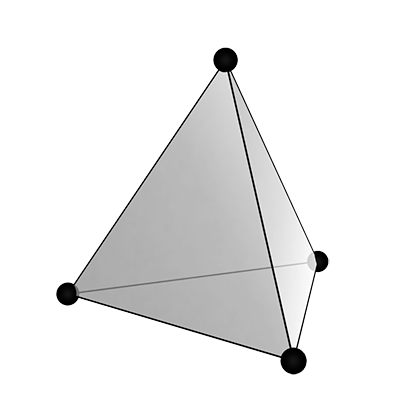
\includegraphics[width=0.23\columnwidth]{P1_tetrahedron.png}}%
\hspace{8pt}%
\subfloat[][$\mathcal{P}^-_1\Omega^1(T)$]{%
	\label{fig:whitney1}%
	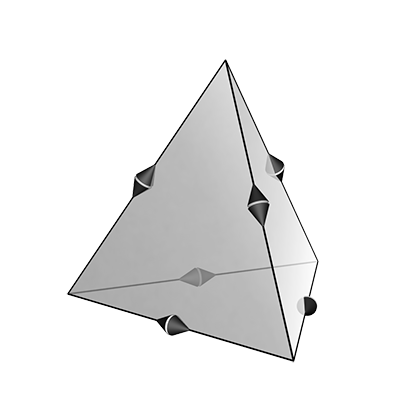
\includegraphics[width=0.23\columnwidth]{N1e1_tetrahedron.png}}%
\hspace{8pt}%
\subfloat[][$\mathcal{P}^-_1\Omega^2(T)$]{%
	\label{fig:whitney2}%
	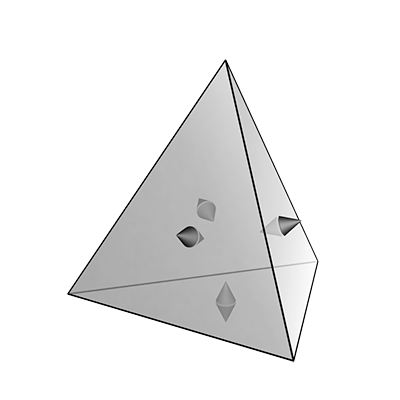
\includegraphics[width=0.23\columnwidth]{N1f1_tetrahedron.png}}
	\hspace{8pt}%
\subfloat[][$\mathcal{P}^-_1\Omega^3(T)$]{%
	\label{fig:whitney3}%
	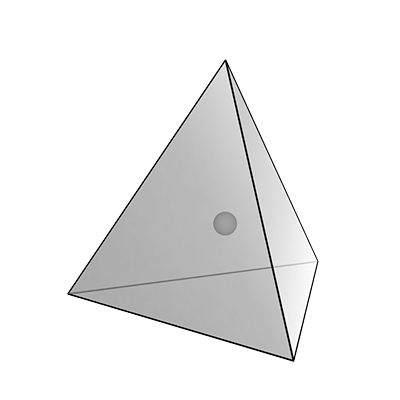
\includegraphics[width=0.23\columnwidth]{dP0_tetrahedron.png}}
\caption{The Whitney forms degrees of freedom in three dimensions (taken from \cite[Page 91]{arnold2018finite})}%
\label{fig:whitneyforms}%
\end{figure}

\subsubsection{Whitney forms}
The Whitney forms are the 
oldest finite elements for differential forms, as they were introduced by Whitney in the fifties \cite{whitney1957}. Whitney forms are constructed by composing the de Rham map and the Whitney interpolation. The de Rham map represents a reduction, since it converts a form into a cochain. The interpolation instead reconstructs a differential form from a cochain.  The space of $k-$cochains over the mesh $\mathcal{T}_h$ is denoted by $C^k(\mathcal{T}_h)$ and the set of $k-$simplexes by $\Delta_k(\mathcal{T}_h)$.

\begin{definition}[de Rham map]
Given a $k$-simplex $\sigma_k^j \in \Delta_k(\mathcal{T}_h)$, the de Rham map is defined as
\begin{equation*}
    \mathcal{R}^k:
\Omega^k(M) \rightarrow C^k(\mathcal{T}_h) ; \qquad \omega^k \mapsto  a^k:=
\sum_{j=1}^{\# \Delta_k(\mathcal{T}_h)}
\dual{\sigma}_k^j
 \int_{\sigma_k^j} \tr_{\sigma_k^j} \omega^k
\end{equation*}
where $\tr_{\sigma_k^j}:=\iota_k^*$ is the pullback of the inclusion map $\iota_k: \sigma_k^j \rightarrow \mathcal{T}_h$
and $\dual{\sigma}_k^j \in C^k$ is the dual basis of $\sigma_k^j \in C_k$.
\end{definition}

\begin{definition}[Whitney interpolation]
Let $\lambda_i:\bbR^n \rightarrow \bbR$
be the barycentric function associated to the vertex $\mathbf{p}_i$ in the 
simplicial complex $\mathcal{T}_h$ representing the computational mesh
(i.e. the unique linear function satisfying $\lambda_i(\mathbf{p}_j) = \delta_{ij}$). \\
The Whitney basis function $w_j^k$ associated to the simplex $\sigma_k^j = [\mathbf{p}_0, \dots, \mathbf{p}_k]$ is computed as
\begin{equation}
    w^k_j := k! \sum_{i=0}^k (-1)^i \lambda_i \d\lambda_0 \wedge \dots \widetilde{\d\lambda}_i \wedge \dots \wedge \d\lambda_k,
\end{equation}
where $\widetilde{\d\lambda}_i$ indicates that $\d\lambda_i$ is omitted. The Whitney interpolation $\mathcal{I}^k$ is the map
\begin{equation*}
    \mathcal{I}^k:
  C^k(\mathcal{T}_h) \rightarrow \Omega^k(M) ; \qquad 
    a^k \mapsto \omega^k_h:= \sum_{j=1}^{\# \Delta_k(\mathcal{T}_h)}  \dualpr[C_k]{a^k}{\sigma_k^j} w^k_j.
\end{equation*}
\end{definition}
The Whitney interpolation is a conforming map. This means that its range is a subspace of the Sobolev space $H\Omega^k(M)$, i.e. $\text{ran}(\mathcal{I}^k)=\text{span}(w^k_1 \hdots w^k_{\#\Delta_k(\mathcal{T}_h)})
\subset H\Omega^k(M)$. A proof of this statement can be found in \cite[Theorem 4.4.]{gillette2011stability}. The range of the Whitney interpolation corresponds to the lowest order trimmed polynomial space $\text{range}(\mathcal{I}^k) = \mathcal{P}^{-}_1\Omega^k(\mathcal{T}_h)$. The following commutativity properties are of fundamental importance for discretization. We consider forms belonging to the domain of the exterior derivative 
%the 
space~$H\Omega^k(M)$. 
\begin{theorem}\cite[Section IV.27]{whitney1957}\label{th:cd_RI}
The following commutativity relations hold for the de Rham map and Whitney interpolation 

\begin{enumerate}
\item $\mathcal{R}^{k+1} \d^k = \partial^k \mathcal{R}^k;$
\item $\d^k \mathcal{I}^k = \mathcal{I}^{k+1} \partial^k$ (Conforming operator).
\end{enumerate}
\begin{figure}[h]
\centering
\begin{tikzcd}
H\Omega^k(M) \arrow[r, "\d^k"] \arrow[d, "\mathcal{R}^k"]
& H\Omega^{k+1}(M) \arrow[d, "\mathcal{R}^{k+1}"] \\
C^k(\mathcal{T}_h) \arrow[r, "\partial^k"]
& C^{k+1}(\mathcal{T}_h)
\end{tikzcd} \hspace{1cm}
\begin{tikzcd}
C^k(\mathcal{T}_h) \arrow[r, "\partial^k"] \arrow[d, "\mathcal{I}^k"]
& C^{k+1}(\mathcal{T}_h) \arrow[d, "\mathcal{I}^{k+1}"] \\
\mathcal{P}^{-}_1\Omega^k(\mathcal{T}_h) \arrow[r, "\d^k"] 
& \mathcal{P}^{-}_1\Omega^{k+1}(\mathcal{T}_h)  
\end{tikzcd} 
\caption{Commuting diagrams for the de Rham map (left) and  Whitney interpolation (right).}
\label{fig:cd_RI}
\end{figure}

\end{theorem}

Given a generic $k$-form $\omega$, one can consider its projection onto the Whitney forms  by composing the de Rham map   and the Whitney interpolation~$\mathcal{I}^k \circ \mathcal{R}^k$~\cite{bochev2006}
\begin{equation}
\Pi_{1, h}^{-, k}:H\Omega^k(M) \rightarrow 
 \mathcal{P}^{-}_1\Omega^{k}(\mathcal{T}_h) 
; \qquad \omega^k \mapsto \omega_h^k:=(\mathcal{I}^k \circ \mathcal{R}^k )(\omega)
\end{equation}
$\Pi^{-, k}_{1, h}$ corresponds to a linear projector from the functional space $H\Omega^k(M) $ to the (finite-dimensional) functional subspace formed by the image of the Whitney forms. The error in the projection represents the error due to the interpolation and can be expressed by means of an $L^2$ inner product:
\begin{equation}\label{eq:L2err}
   \text{Err}(\omega):
H\Omega^k(M) \rightarrow \mathbb{R} ; \qquad 
\omega \mapsto \inpr[M]{\omega-\Pi_{1, h}^{-, k}(\omega)}{\omega-\Pi_{1, h}^{-, k}(\omega)} 
\end{equation}

An immediate corollary of Theorem~\ref{th:cd_RI} is that the commutativity property extends to the projector 
\begin{equation*}
\d^k \Pi_{1, h}^k = \Pi_{1, h}^{k+1}\d^k.    
\end{equation*}
This property, that goes under the name of {\it cochain property} \cite{arnold2018finite}, is fundamental and common to all the different families of finite element differential forms. It basically represents the compatibility and preservation of the differential structure in the subspace of the projection, it basically shows that $\Pi_{1, h}^{-, k}$ is a structure preserving map with the structure being the topological one represented by $\d^k$. It is important to realise that the particularity of the Whitney forms resides in the fact that the commutativity property holds at the level of both the interpolation and the reduction map. This is due to the fact that Whitney forms are highly geometrical, since they associate to each $k$-dimensional subsimplex only one degree of freedom as illustrated before.

\subsubsection{Higher order elements}
It is now possible to generalise the Whitney forms as first order finite elements to the case of higher order $s>1$. This may be done by introducing  conforming finite element families arising from the Finite Element Exterior Calculus framework. As we have seen previously, for a $s$ order finite element method, we can associate to each element $\mathrm{dim}( \mathcal{P}^-_s\Omega^k(T))$ basis forms. Higher order cases of the trimmed polynomial spaces are constructed by defining extra degrees of freedom (reported in Eq. \eqref{eq:dof_P-} in \ref{app:ho_feec}) in the finite element. The general construction of the
polynomial spaces of differential forms is given in \cite{arnold2006acta}, and summarized in \ref{app:ho_feec} for the reader's convenience. 

\section{The primal-adjoint Stokes-Dirac structure}\label{sec:pradj_SDS}
In this section the strong formulation of port-Hamiltonian systems and the important role of the underlying geometrical structure are recalled. The corresponding adjoint system is constructed.

\subsection{Linear Stokes-Dirac structures}
In the classical case of a system of dual conserving quantities, such as wave propagation phenomena, the setting can be framed in the following way with hyperbolic PDEs. Given a smooth manifold $M$ of dimension $n$, the flux variables ${f}^p \in \Omega^p(M), \; {f}^q \in \Omega^q(M)$ and the effort variables ${e}^p \in \Omega^{n-p}(M), \; {e}^q \in \Omega^{n-q}(M)$, with\footnote{This relation in dimensions is due to the fact that the fields are dual and will become clear from the construction hereafter.} $p+q=n+1$, consider the Stokes-Dirac structure

\begin{equation}\label{eq:StokesDirac}
    \begin{pmatrix}
        {f}^p \\
        {f}^q
    \end{pmatrix} = 
    \underbrace{\begin{bmatrix}
    0 & (-1)^r \d \\
    \d & 0 \\
    \end{bmatrix}}_{J}
    \begin{pmatrix}
        {e}^p \\
        {e}^q
    \end{pmatrix}, \qquad 
    \begin{pmatrix}
        {f}^\partial \\
        {e}^\partial
    \end{pmatrix} = 
    \begin{bmatrix}
    \tr & 0 \\
    0 &  (-1)^p\tr
    \end{bmatrix}
    \begin{pmatrix}
        {e}^p \\
        {e}^q
    \end{pmatrix},
\end{equation}
where $r = pq +1$ for mathematical and physical reasons \cite{vanderSchaft2002}. The operator $J$, representing what is called in physical system theory the junction structure, is called the interconnection operator and is a formally skew-adjoint operator.  This property is at the core of the balance equation
\begin{equation}\label{eq:bal_eq}
    \dualpr[M]{e^p}{f^p} + \dualpr[M]{e^q}{f^q} + \dualpr[\partial M]{e^\partial}{f^\partial} = 0,
\end{equation}
where $\partial M$ denotes the boundary of manifold $M$. 
This balance equation arises from the application of the Leibniz rule and the Stokes theorem and states the overall conservation of energy.
This is the  embodiment of Tellegen's theorem generalised to the  distributed parameters systems case \cite{iftime2014kernel}.


\subsection{Port-Hamiltonian systems}
Port-Hamiltonian systems encoding conservation laws are associated to the geometrical Stokes-Dirac structure. To establish this connection, consider the distributed state variables $\alpha^p
%(\xi, t) 
\in \Omega^p(M), \; \alpha^q
%(\xi, t) 
\in \Omega^q(M)$ and the Hamiltonian functional 
\begin{equation}\label{eq:H}
H(\alpha^p
%(\xi, t)
, \alpha^q
%(\xi, t)
) = \int_M
\mathcal{H}(\alpha^p
%(\xi, t)
, \alpha^q
%(\xi, t)
)
\end{equation}
with Hamiltonian density $n$-form $\mathcal{H}$. A fundamental notion is the variational derivative of the Hamiltonian functional \cite{olver1986applications, vanderSchaft2002}. 
\begin{definition}[Variational derivative]\label{def:var_der}
The variational derivatives of the Hamiltonian $\delta_{p} H, \; \delta_{q} H$ are defined implicitly by
\begin{equation*}
\begin{aligned}
    \left.\diff{}{\varepsilon}\right|_{\varepsilon = 0} H(\alpha^p + \varepsilon \delta \alpha^p, \alpha^q) = \dualpr[M]{\delta_{p} H}{\delta \alpha^p}, \\
    \left.\diff{}{\varepsilon}\right|_{\varepsilon = 0} H(\alpha^p, \alpha^q + \varepsilon \delta \alpha^q) = \dualpr[M]{\delta_{q} H}{\delta \alpha^q}.
\end{aligned}
\end{equation*}
\end{definition}

Considering than a trajectory $(\alpha_p(t),\alpha_q(t))$ parameterised by time in the manifold of state fields, the variational derivative is defined so that the rate of the Hamiltonian \eqref{eq:H} reads
\begin{equation}\label{eq:H_dot}
    \dot{H} = \dualpr[M]{\delta_{p} H}{\partial_t \alpha_p} + \dualpr[M]{\delta_{q} H}{\partial_t \alpha_q}.
\end{equation}

Consider then the following equations which can be seen to represent a system of two conservation laws with canonical inter-domain coupling \cite{vanderSchaft2002}. With an abuse of notation, indicating 
$\alpha^\bullet(\xi, t)= (\alpha^\bullet (t))(\xi)$ to make explicit the value of the field at a certain location rather than the field as a section
\begin{equation}\label{eq:pHsys}
    \begin{pmatrix}
        \partial_t \alpha^p(\xi, t) \\
        \partial_t \alpha^q(\xi, t) \\
    \end{pmatrix} = -
    \begin{bmatrix}
    0 & (-1)^r \d \\
    \d & 0 \\
    \end{bmatrix}
    \begin{pmatrix}
        \delta_{p} H \\
        \delta_{q} H
    \end{pmatrix}, \qquad 
    \begin{pmatrix}
        {f}^\partial \\
        {e}^\partial
    \end{pmatrix} = 
    \begin{bmatrix}
    \tr & 0 \\
    0 &  (-1)^p\tr
    \end{bmatrix}
    \begin{pmatrix}
        \delta_{p} H \\
        \delta_{q} H
    \end{pmatrix},  
\end{equation}
with initial conditions
\begin{equation}
    \begin{pmatrix}
        \alpha^p(\xi, 0) \\
        \alpha^q(\xi, 0)
    \end{pmatrix} = 
    \begin{pmatrix}
        \alpha^p_0(\xi) \\
        \alpha^q_0(\xi) \\
    \end{pmatrix}.
\end{equation}
The flows and efforts of the associated Stokes-Dirac 
structure \eqref{eq:StokesDirac} are then defined by
\begin{equation}\label{eq:pHsys_flows_efforts}
\begin{pmatrix}
        f^p \\
        f^q
    \end{pmatrix} :=
    \begin{pmatrix}
        -\partial_t \alpha^p(\xi, t) \\
        -\partial_t \alpha^q(\xi, t) \\
    \end{pmatrix}, \qquad 
    \begin{pmatrix}
        e^p \\
        e^q
    \end{pmatrix} = 
    \begin{pmatrix}
        \delta_{p} H \\
        \delta_{q} H
    \end{pmatrix}.
\end{equation}
Given the balance equation \eqref{eq:bal_eq}, the rate of change of Hamiltonian (power flow) reads
\begin{equation}\label{eq:powbal}
    \dot{H} = \dualpr[\partial M]{e^\partial}{f^\partial},
\end{equation}
which states that the change of energy within the spatial domain $M$ is equal to the supplied power through its boundary $\partial M$.

\paragraph{Constitutive equations}
Since in this work the focus is on the case in which the closure equations are linear, we make the additional assumption of a quadratic Hamiltonian.
\begin{assumption}[Quadratic Hamiltonian]\label{ass:quad_Ham}
The Hamiltonian density in assumed to be quadratic in the state variables
\begin{equation}\label{eq:H_den}
\mathcal{H}(\alpha^p, \alpha^q) = 
    \frac{1}{2} A^p \alpha^p \wedge \star \alpha^p + \frac{1}{2}  A^q \alpha^q \wedge \star  \alpha^q,
\end{equation}
where $A^p: L^2\Omega^{p}(M) \rightarrow L^2\Omega^{p}(M)$ and $A^q: L^2\Omega^{q}(M) \rightarrow L^2\Omega^{q}(M)$ are bounded, symmetric, positive definite operators with respect to the standard inner products in $L^2$. These tensors are related to physical properties of space like electric permittivity, density or Young modulus.
\end{assumption}
Because of this assumption, the variational derivatives of the Hamiltonian, computed according to Definition \ref{def:var_der}, can be seen to be
\begin{equation}
    \delta_{p} H = (-1)^{p(n-p)}\star A^p\alpha^p, \qquad
    \delta_{q} H = (-1)^{q(n-q)}\star A^q\alpha^q.
\end{equation} 

\paragraph{Boundary conditions}
The actual boundary conditions for a problem at hand are then accounted for by considering the causally dual
(input-output) behavior of the system. We denote with $\Gamma_p$  and $\Gamma_q$ two open subset of the boundary that   verify $\overline{\Gamma}_p \cup \overline{\Gamma}_q = \partial M$ and $\Gamma_p \cap \Gamma_q=\emptyset$. Each boundary subpartition is associated with one boundary condition. In particular, the values of $e^p$ and $e^q$ are imposed on $\Gamma_p$ and $\Gamma_q$, respectively. Since in this paper we consider boundary controlled systems, the values taken by $e^p$ and $e^q$ are assigned by means of the inputs
 \begin{equation}\label{eq:u}
    \tr e^p \vert_{\Gamma_p} = u^p, \qquad
    (-1)^p \tr e^q \vert_{\Gamma_q} = u^q.
 \end{equation}
The outputs are defined in a complementary manner as follows
 \begin{equation}\label{eq:y}
    y^p := \tr e^p \vert_{\Gamma_q}, \qquad
    y^q := (-1)^p \tr e^q \vert_{\Gamma_p}. 
 \end{equation}
Given this definition and the additive property of the integration, we can express the supplied energy through $\partial M$ as
\begin{equation}
    \dualpr[\partial M]{e^\partial}{f^\partial} =   \dualpr[\Gamma_p]{y^q}{u^p} + \dualpr[\Gamma_q]{u^q}{y^p}.
\end{equation}

\subsection{Adjoint Stokes-Dirac structure \label{sec:asds}}

The port-Hamiltonian system (\ref{eq:pHsys}) and its associated Stokes-Dirac structure (\ref{eq:StokesDirac}) were defined on the state space denoted by $X = \Omega^p(M) \times \Omega^q(M)$. The key ingredient that will be used for discretization is the Adjoint Stokes-Sirac structure that we will introduce in this section. This adjoint structure is defined on the dual state space $\dual{X} = \Omega^{n-p}(M) \times \Omega^{n-q}(M)$ related to $X$ by the diffeomorphism

\begin{equation}\label{eq:Phi_Diffeo}
	\Phi:
	X \rightarrow \dual{X} ; \qquad
	(\alpha^p, \alpha^q) \mapsto (\star\alpha^p, \star \alpha^q).
\end{equation}

It is worth noting that the choice of $\Phi$ is not unique. While in this work we choose (\ref{eq:Phi_Diffeo})  for numerical reasons, in Sec. \ref{sec:additionalinsights} we will discuss an alternative that is defined in a slightly different way which is much closer to the physics of the problem and gives some new insights.

The pushforward associated to the diffeomorphism converts elements in the tangent space of the state space
\begin{equation}\label{eq:pushfor_phi}
\Phi_* : T X \rightarrow T \dual{X}; \qquad     (f^p, f^q) 
\mapsto  (\star f^p, \star f^q).
\end{equation}



\begin{remark}
Since the space of differential forms is an infinite dimensional $\bbR$ vector space, the tangent space  is actually isomorphic with the space of forms: $TX = T\Omega^p \times T\Omega^q \cong \Omega^p \times \Omega^q$. 
\end{remark}
\begin{proposition}\label{pr:pullback_phi}
The pullback $\Phi^*$ of the map $\Phi$ is given by:
\begin{equation}
\label{eq:pullback_phi}
\Phi^*: T^*_{\dual{x}} \dual{X} \cong \dual{X} \rightarrow T^*_x X \cong X: 
(\dual{e}^p, \dual{e}^q) \mapsto ((-1)^{p(n-p)}\star \dual{e}^p, \; (-1)^{q(n-q)}\star \dual{e}^q) 
\end{equation}
\end{proposition}
\begin{proof}
The pullback is defined by duality
\begin{equation}
    \dualpr[X]{\Phi^* (\dual{e}^p, \dual{e}^q)}{(f^p, f^q)} = \dualpr[\dual{X}]{(\dual{e}^p, \dual{e}^q)}{\Phi_*(f^p, f^q)}.
\end{equation}
Using the definition of duality product \eqref{eq:dual_pr} one obtains
\begin{equation}
    \begin{aligned}
    \dualpr[\dual{X}]{(\dual{e}^p, \dual{e}^q)}{\Phi_*(f^p, f^q)} &=\int_M \dual{e}^p \wedge \star f^p + \int_M \dual{e}^q \wedge \star f^q, \\
        &= \int_M (-1)^{p(n-p)}\star \dual{e}^p \wedge f^p + \int_M (-1)^{q(n-q)}\star \dual{e}^q \wedge f^q, \\
        &=  \dualpr[X]{((-1)^{p(n-p)}\star \dual{e}^p, (-1)^{q(n-q)}\star \dual{e}^q)}{(f^p, f^q)}
    \end{aligned}
\end{equation}
\end{proof}

\begin{comment}
\begin{equation}
    \begin{pmatrix}
    \dual{f}^{p} \\
    \dual{f}^{q} 
    \end{pmatrix} = 
    \begin{bmatrix}
        0 &  (-1)^{r + q(n-q)}{\star} \d{} {\star} \\
        (-1)^{p(n-p)}{\star} \d{} {\star} & 0 \\
    \end{bmatrix}
    \begin{pmatrix}
        \dual{e}^{p}\\
        \dual{e}^{q}
    \end{pmatrix}, \qquad 
    \begin{pmatrix}
        {f}^\partial \\
        {e}^\partial
    \end{pmatrix} = 
    \begin{bmatrix}
    \tr  & 0 \\
    0 &  (-1)^{p}\tr 
    \end{bmatrix}
    \begin{pmatrix}
        {e}^{p}\\
        {e}^{q}
    \end{pmatrix}.
\end{equation}
\end{comment}

By introducing $(\dual{f}^{p},\dual{f}^{q}) := \Phi_*(f^p,f^q)$ and $ (e^p,e^q)= \Phi^*(\dual{e}^{p},\dual{e}^{q})$, the Stokes-Dirac structure \eqref{eq:StokesDirac} is equivalently rewritten 
in terms of the co-differential map $\d^*$ defined in eq. \eqref{eq:codif}:
\begin{equation}\label{eq:AdjStokesDirac}
    \begin{pmatrix}
    \dual{f}^{p} \\
    \dual{f}^{q} 
    \end{pmatrix} = 
    \begin{bmatrix}
        0 &  (-1)^{a_0}\d{}^* \\
        (-1)^{a_1}\d{}^* & 0 \\
    \end{bmatrix}
    \begin{pmatrix}
        \dual{e}^{p}\\
        \dual{e}^{q}
    \end{pmatrix}, \qquad 
    \begin{pmatrix}
        {f}^\partial \\
        {e}^\partial
    \end{pmatrix} = 
    \begin{bmatrix}
    (-1)^{p(n-p)} \tr \star & 0 \\
    0 &  (-1)^{p+q(n-q)}\tr \star
    \end{bmatrix}
    \begin{pmatrix}
        \dual{e}^{p}\\
        \dual{e}^{q}
    \end{pmatrix},
\end{equation}
where the following notation has been used
\begin{equation}\label{eq:a_coeff}
    a_0 = r + q(n-q) + nq + n +1, \qquad a_1 = p(n-p) + np + n +1.
\end{equation}

From Prop. \ref{pr:pullback_phi} the following corollary is deduced.
\begin{corollary}\label{cor:pow_bal_Adj}
The adjoint Stokes-Dirac structure verifies the power balance
\begin{equation}\label{eq:pow_bal_Adj}
    \dualpr[M]{\dual{e}^p}{\dual{f}^p} + \dualpr[M]{\dual{e}^q}{\dual{f}^q} + \dualpr[\partial M]{e^\partial}{f^\partial} = 0.
\end{equation}
\end{corollary}

\begin{proof}
    The property follows from the fact that the pullback \eqref{eq:pullback_phi} preserves duality products. It can be  verified by a direct computation that:
    \begin{equation}
    \begin{aligned}
    \dualpr[M]{e^p}{f^p} &= \int_M \star \dual{e}^p \wedge \star \dual{f}^p, \qquad &\text{Symmetry of the inner product}, \\
    &= \int_M \dual{f}^p \wedge \star (\star \dual{e}^p), \qquad &\text{Property of the the Hodge star}, \\
    &= (-1)^{p(n-p)} \int_M \dual{f}^p \wedge  \dual{e}^p, \qquad &\text{Skew-symmetry of the wedge},  \\
    &= \dualpr[M]{\dual{e}^p}{\dual{f}^p}.
    \end{aligned} 
\end{equation}
Analogous computations are performed for the $q$ flux and effort $f^q$ and $e^q$.
\end{proof}
To simplify the expressions of the adjoint Dirac structure and relate the new indices $a_0$ and $a_1$ to the $p,q,n$, the following proposition is of value.
\begin{proposition}\label{pr:parity_a0_a1}
The coefficients $a_0 + 1, \;p(n-p)$ and $a_1 + 1 +r, \; q(n-q)$ have the same parity which means
\begin{equation}
    a_0 + 1 \equiv p(n-p) \mod{2}, \qquad a_1 + 1 + r \equiv q(n-q) \mod{2}.
\end{equation}
where $\mod{2}$ denotes the modulo of the division by $2$.
\end{proposition}
\begin{proof}
Reported in \ref{app:proofs}.
\end{proof}
\noindent This results implies that:
\[
(-1)^{a_0}=(-1)^{p(n-p)+1}
\qquad \text{and}
\qquad
(-1)^{a_1}=(-1)^{q(n-q)+r+1}
\]
and this could be used to express \eqref{eq:AdjStokesDirac} with the coefficients $p,q,n$ and $r$, and will be of importance later. The adjoint Stokes-Dirac structure introduces the codifferential and its important role in discretization. 

\subsection{Associated port-Hamiltonian adjoint system}

Given the adjoint Stokes-Dirac structure \eqref{eq:AdjStokesDirac} and the pH system \eqref{eq:pHsys}, the adjoint pH system is obtained by considering the isomorphism
\[ (\dual{\alpha}^p,\dual{\alpha}^q) := \Phi(\alpha^p,\alpha^q) = (\star \alpha^p, \star \alpha^q) ,\]
and considering the new Hamiltonian as a function of the dual state variables
\begin{equation}
   \dual{H}(\dual{\alpha}^p(\xi, t), \dual{\alpha}^q(\xi, t)) = 
\int_M   \dual{\mathcal{H}}(\dual{\alpha}^p(\xi, t), \dual{\alpha}^q(\xi, t), \xi).
\end{equation}
The energy density $\dual{\mathcal{H}}$ corresponds to $\mathcal{H}$ under the isomorphism $\Phi$. The variational derivative, being defined by duality product (cf. Def. \ref{def:var_der}), undergoes the same pullback as the efforts, so that
\begin{equation}\label{eq:dual_coenergies}
    \diffd{\dual{H}}{\dual{\alpha}^p} = \dual{e}^p, \qquad  \diffd{\dual{H}}{\dual{\alpha}^q} = \dual{e}^q.
\end{equation}

The port-Hamiltonian adjoint system is obtained substituting into the adjoint Stokes-Dirac structure \eqref{eq:AdjStokesDirac} the dual fluxes 
\begin{equation}\label{eq:dual_flows}
\dual{f}^p = - \partial_t \dual{\alpha}^p, \qquad \dual{f}^q = - \partial_t \dual{\alpha}^q,   
\end{equation}
and efforts \eqref{eq:dual_coenergies}
\begin{equation}\label{eq:AdjPHsys}
    \begin{pmatrix}
        \partial_t \dual{\alpha}^p(\xi, t) \\
        \partial_t \dual{\alpha}^q(\xi, t) \\
    \end{pmatrix} = -
    \begin{bmatrix}
        0 &  (-1)^{a_0}\d{}^* \\
        (-1)^{a_1}\d{}^* & 0 \\
    \end{bmatrix}
    \begin{pmatrix}
        \delta_{\dual{p}} \dual{H} \\
        \delta_{\dual{q}} \dual{H}
    \end{pmatrix}.
\end{equation}

Given Assumption \ref{ass:quad_Ham}, the dual energy is a quadratic function in the dual state variables
\begin{equation*}
    \dual{\mathcal{H}}(\dual{\alpha}^p(\xi, t), \dual{\alpha}^q(\xi, t)) = \frac{1}{2} \dual{A}^p \dual{\alpha}^p \wedge \star \dual{\alpha}^p + \frac{1}{2} \dual{A}^q \dual{\alpha}^q \wedge \star  \dual{\alpha}^q,
\end{equation*}
where the dual operators $\dual{A}^p, \; \dual{A}^q$, defined implicitly by
\begin{equation}
\begin{aligned}
    \dualpr[M]{A^p\alpha^p}{\dual{\alpha}^p} &= \dualpr[M]{\alpha^p}{\dual{A}^p \dual{\alpha}^p}, \\
    \dualpr[M]{A^q\alpha^q}{\dual{\alpha}^q} &= \dualpr[M]{\alpha^q}{\dual{A}^q \dual{\alpha}^q},
\end{aligned}
\end{equation}
are bounded, symmetric and positive definite with respect to the $L^2$ inner product. Furthermore they verify the commutativity property $\star A^p = \dual{A}^p \star, \; \star A^q = \dual{A}^p \star$, thus are explicitly expressed by
\begin{equation}
    \dual{A}^p = (-1)^{p(n-p)} \star A^p \star, \qquad \dual{A}^q = (-1)^{q(n-q)} \star A^q \star.
\end{equation}

The variational derivative of the dual energy then reads
\begin{equation}
    \delta_{\dual{p}} \dual{H} = (-1)^{p(n-p)} \star  \dual{A}^p\dual{\alpha}^p, \qquad
    \delta_{\dual{q}} \dual{H} = (-1)^{q(n-q)} \star \dual{A}^q \dual{\alpha}^q.
\end{equation} 
For what concerns the boundary conditions, it is important to notice that the adjoint system carries the same boundary conditions \eqref{eq:u} as the primal one, but expressed by means of the dual efforts
 \begin{equation}
    (-1)^{p(n-p)}\tr\star \dual{e}^p \vert_{\Gamma_p} = u^p, \qquad
    (-1)^{pq(n-q)} \tr \star \dual{e}^q \vert_{\Gamma_q} = u^q.
 \end{equation}
and analogously for the outputs.

\section{Weak dual field formulation}\label{sec:weak_df}

We now present the weak dual field formulation of the port-Hamiltonian model, inspired by the work of \cite{zhang2021mass}. In this formulation, we combine together the primal and adjoint port-Hamiltonian systems described in the previous section. This combination will eliminate the necessity of using an explicit Hodge star operator, which will be accounted for instead using the weak adjoint system and the integration by parts formula \eqref{eq:intbyparts_codif}.

\subsection{Motivation of the approach}

The novelty of this approach is that the Hamiltonian can now be rewritten as a function of the primal and dual state variables:
 \begin{equation}
H_T(\alpha^p, \alpha^q, \dual{\alpha}^p, \dual{\alpha}^q) = H(\alpha^p, \alpha^q) + \dual{H}(\dual{\alpha}^p, \dual{\alpha}^q)= \int_M \mathcal{H}_T,
\end{equation}
with associated density
\begin{equation*}
\mathcal{H}_T
(\alpha^p, \alpha^q 
,\dual{\alpha}^p, \dual{\alpha}^q) 
= A^p \alpha^p \wedge \dual{\alpha}^p 
+ A^q \alpha^q \wedge \dual{\alpha}^q.    
\end{equation*}
The Hamiltonian density depends on four variables related by duality and the Hodge star has been removed. This is important because the discretisation can be performed without relying on a discrete Hodge star. The primal and dual efforts are related to the dual and primal state by
\begin{equation}
\begin{aligned}
    e^p = \diffd{H_T}{\alpha^p} = (-1)^{p(n-p)} \dual{A}^p \dual{\alpha}^p, \\
    e^q = \diffd{H_T}{\alpha^q} = (-1)^{q(n-q)} \dual{A}^q \dual{\alpha}^q, \\
\end{aligned} \qquad \qquad
\begin{aligned}
    \dual{e}^p = \diffd{H_T}{\dual{\alpha}^p} = A^p \alpha^p, \\
    \dual{e}^q = \diffd{H_T}{\dual{\alpha}^q} = A^q \alpha^q. \\
\end{aligned}
\end{equation}
The constitutive equations are then incorporated directly in the dynamics by reducing the state variables in terms of the efforts \cite{brugnoli2020}. This reduces the number of equations to be solved and formulate the problem in terms of the most important variables, as the efforts are subjected to the boundary conditions.


\subsection{Constitutive equations}

The primal and dual effort variables are then expressed in weak form by inverting the material operators $A^p, \dual{A}^p, A^q, \dual{A}^q$
\begin{equation}\label{eq:weak_CE}
     \begin{aligned}
     \inpr[M]{{v}^p}{\alpha^p} &= \inpr[M]{{v}^p}{C^p \dual{e}^p}, \\
      \inpr[M]{{v}^q}{\alpha^q} &= \inpr[M]{{v}^q}{C^q \dual{e}^q}, \\
      \inpr[M]{\dual{v}^p}{\dual{\alpha}^p} &= \inpr[M]{\dual{v}^p}{(-1)^{p(n-p)} \dual{C}^p e^p}, \\
      \inpr[M]{\dual{v}^q}{\dual{\alpha}^q} &= \inpr[M]{\dual{v}^q}{(-1)^{q(n-q)} \dual{C}^q e^q}, 
     \end{aligned} \qquad 
     \begin{aligned}
     \forall v^p &\in H\Omega^p(M), \\
     \forall v^q &\in H\Omega^q(M), \\
     \forall \dual{v}^p &\in H\Omega^{q-1}(M), \\
     \forall \dual{v}^q &\in H\Omega^{p-1}(M), \\
     \end{aligned}
\end{equation}
where the tensors $C^p:= (A^p)^{-1}, \; C^q := (A^q)^{-1}, \; \dual{C}^p :=(\dual{A}^p)^{-1} = (-1)^{p(n-p)}\star (A^p)^{-1} \star, \; \dual{C}^q := (\dual{A}^q)^{-1} = (-1)^{q(n-q)}\star (A^q)^{-1} \star$ have been introduced. These tensors are commonly introduced in mixed finite element (for example in linear elasticity they represent the density and the compliance \cite{arnold2014weak}, whereas in electromagnetism they represent the electric permittivity and the magnetic permeability \cite{asad2019maxwell}). By introducing the energy $H_T$, it is possible to eliminate the need for a discrete Hodge star, at least in the linear case. However, the strength of the approach is not limited to the linear case: in \cite{zhang2021mass}, the construction of the adjoint system allows dealing with the non linear gyroscopic term in the Navier-Stokes equation in a linear fashion, by relying on the vorticity information from the dual system. 

\begin{remark}\label{rmk:dualelimination}
By using \eqref{eq:weak_CE}, the final dynamical system can  be expressed in terms of the efforts only. Other equivalent reduction may get rid of the dual variables by considering
\begin{equation*}
     \begin{aligned}
     \inpr[M]{{v}^p}{\dual{e}^p} &= \inpr[M]{{v}^p}{A^p\alpha^p}, \\
      \inpr[M]{{v}^q}{\dual{e}^q} &= \inpr[M]{{v}^q}{A^q\alpha^q}, \\
      \inpr[M]{\dual{v}^p}{\dual{\alpha}^p} &= \inpr[M]{\dual{v}^p}{(-1)^{p(n-p)} \dual{C}^p e^p}, \\
      \inpr[M]{\dual{v}^q}{\dual{\alpha}^q} &= \inpr[M]{\dual{v}^q}{(-1)^{q(n-q)} \dual{C}^q e^q}.
     \end{aligned}
\end{equation*}
\end{remark}


\subsection{Dual field Stokes-Dirac structure}
Now we will present the dual field Stokes-Dirac structure which will be constructed by combining the Stokes-Dirac structure \eqref{eq:StokesDirac} and its adjoint \eqref{eq:AdjStokesDirac}. In order to obtain the weak form, we take the inner product of (\eqref{eq:StokesDirac}) and \eqref{eq:AdjStokesDirac} with test differential forms of appropriate degrees and use the integration by parts formula \eqref{eq:intbyparts_codif} for the adjoint system. Consequently, if we let $\mathcal{F}:= H\Omega^p(M)\times H\Omega^q(M) \times H\Omega^{q-1}(M) \times H\Omega^{p-1}(M)$, then the weak form of the dual-field Stokes-Dirac structure is given by the subspace $\mathcal{D} \subset \mathcal{F}\times \mathcal{F}^*$, such that for $(f^p,f^q,\dual{f}^p,\dual{f}^q)\in \mathcal{F}$ and $(e^p,e^q,\dual{e}^p,\dual{e}^q)\in \mathcal{F}^*$ we have that:

 \begin{equation}\label{eq:weak_dfSDS}
    \begin{aligned}
    \inpr[M]{v^p}{f^p} &= \inpr[M]{v^p}{(-1)^r\d e^q}, \\
    \inpr[M]{v^q}{f^q} &= \inpr[M]{v^q}{\d e^p}, \\
    \inpr[M]{\dual{v}^p}{\dual{f}^p} &= \inpr[M]{\d\dual{v}^p}{(-1)^{a_0} \dual{e}^q} - \dualpr[\partial M]{\dual{v}^p}{(-1)^{b_0} e^q}, \\
      \inpr[M]{\dual{v}^q}{\dual{f}^q} &= \inpr[M]{\d\dual{v}^q}{(-1)^{a_1}
      \dual{e}^p} - \dualpr[\partial M]{\dual{v}^q}{(-1)^{b_1} e^p},
    \end{aligned} \qquad
    \begin{aligned}
    f^\partial &= \tr e^p, \\
    e^\partial &=(-1)^p\tr e^q, \\
    \\
    \\
    \end{aligned} \qquad
    \begin{aligned}
    &\forall v^p \in H\Omega^p(M), \\
    &\forall v^q \in H\Omega^q(M). \\
    &\forall\dual{v}^p \in H\Omega^{q-1}(M), \\
    &\forall\dual{v}^q \in H\Omega^{p-1}(M),
    \end{aligned}
\end{equation}
where $ b_0 = r + nq + n + 1, \quad b_1 = np + n +1$ (or $a_0 = b_0 + q(n-q), \quad a_1 = b_1 + p(n-p)$).  Note that since the degree of the different forms are linked by $p+q = n+1$, the degree of the efforts $e^p, \; e^q$ is $q-1, \; p-1$ respectively.

\subsection{Boundary conditions enforcement}\label{subsection:weak_bcs}
A number of different techniques can be used to enforce boundary conditions (cf. \cite{benner2015timebc} and references therein). One technique consists of strong imposition by direct assignment of the boundary degrees of freedom.
Another interesting possibility consists of using a time staggering discretization, as proposed in \cite{zhang2021mass}, together with a weak imposition of the boundary conditions by means of the adjoint port-Hamiltonian systems. By time staggering discretization, we indicate the fact the solution of one system is computed at integer time instants, whereas for the second system, arising from the dual field formulation, the solution is computed at half-integer time instants.

In this paper, we will opt for the strong imposition strategy of boundary conditions as it will ensure that the power flow is correctly represented (up to the approximation error introduced by the polynomial interpolation) as it will be proven later.

\subsection{Overall port-Hamiltonian dynamics} 
Using the weak formulation of the constitutive equation \eqref{eq:weak_CE}, the dynamics is expressed using the efforts variable only. The weak form of the dynamics accounts for the boundary conditions, that will be strongly enforced by considering test functions satisfying homogeneous boundary conditions in the adjoint system. Consider now the definition of the flows \eqref{eq:pHsys_flows_efforts} and dual flows \eqref{eq:dual_flows} and the associated weak formulation
\begin{equation}
    \begin{aligned}
    \inpr[M]{v^p}{f^p} &= -\inpr[M]{v^p}{\partial_t \alpha^p}, \\
    \inpr[M]{\dual{v}^p}{\dual{f}^p} &= -\inpr[M]{\dual{v}^p}{\partial_t \dual{\alpha}^p}, \\
    \end{aligned} \qquad
    \begin{aligned}
    \inpr[M]{v^q}{f^q} &= -\inpr[M]{v^q}{\partial_t \alpha^q}, \\
    \inpr[M]{\dual{v}^q}{\dual{f}^q} &= -\inpr[M]{\dual{v}^q}{\partial_t \dual{\alpha}^p},
    \end{aligned}
\end{equation}
If the weak constitutive equations in Eq. \eqref{eq:weak_CE} are used to express the states and co-states in terms of the efforts one obtains
\begin{equation}
    \begin{aligned}
    \inpr[M]{v^p}{f^p} &= -\inpr[M]{v^p}{C^p \partial_t \dual{e}^p}, \\
    \inpr[M]{\dual{v}^p}{\dual{f}^p} &= -\inpr[M]{\dual{v}^p}{(-1)^{p(n-p)} \dual{C}^p\partial_t e^p}, \\
    \end{aligned} \qquad
    \begin{aligned}
    \inpr[M]{v^q}{f^q} &= -\inpr[M]{v^q}{C^q \partial_t \dual{e}^q}, \\
    \inpr[M]{\dual{v}^q}{\dual{f}^q} &= -\inpr[M]{\dual{v}^q}{(-1)^{q(n-q)} \dual{C}^q\partial_t e^q}.
    \end{aligned}
\end{equation}
Replacing these expressions in the weak formulation \eqref{eq:weak_dfSDS} and
 using Prop. \ref{pr:parity_a0_a1} as well as the relations 
\begin{equation}
    b_0 + p + p(n-p) \equiv (p-1)(q-1) \mod 2, \qquad 
        b_1 + q(n-q) \equiv p \mod 2, 
\end{equation}
the following weak formulation is obtained: find $\dual{e}^p \in H\Omega^{p}, \; \dual{e}^q \in H\Omega^{q}$ and ${e}^p \in H\Omega^{q-1}, \; e^q \in H\Omega^{p-1}$ such that $\tr e^p \vert_{\Gamma_p} = u^p, \; (-1)^p \tr e^q \vert_{\Gamma_q} = u^q$ and
 \begin{equation}\label{eq:weak_dfPHdyn}
    \begin{aligned}
    \inpr[M]{v^p}{C^p \partial_t \dual{e}^p} &= -\inpr[M]{v^p}{(-1)^r\d e^q}, \\
    \inpr[M]{v^q}{C^q \partial_t \dual{e}^q} &= -\inpr[M]{v^q}{\d e^p}, \\
    \inpr[M]{\dual{v}^p}{\dual{C}^p \partial_t e^p} &=\inpr[M]{\d\dual{v}^p}{\dual{e}^q} + \dualpr[\Gamma_q]{\dual{v}^p}{(-1)^{(p-1)(q-1)}u^q}, \\
      \inpr[M]{\dual{v}^q}{\dual{C}^p \partial_t e^p} &= \inpr[M]{\d\dual{v}^q}{(-1)^{r} \dual{e}^p} + \dualpr[\Gamma_p]{\dual{v}^q}{(-1)^{p}u^p}. 
    \end{aligned}  \qquad 
    \begin{aligned}
    &\forall v^p \in H\Omega^p(M), \\
    &\forall v^q \in H\Omega^q(M), \\
    &\forall \dual{v}^p \in H\Omega^{q-1}(M, \Gamma_p), \\
    &\forall \dual{v}^q \in H\Omega^{p-1}(M, \Gamma_q), \\
    \end{aligned}
 \end{equation}
where $H\Omega^{q-1}(M, \Gamma_p)$ and $H\Omega^{p-1}(M, \Gamma_q)$ are the Sobolev spaces with boundary conditions defined as 
\begin{equation}
    \begin{aligned}
        H\Omega^{q-1}(M, \Gamma_p) &:= \{w \in H\Omega^{q-1}(M) \vert \; \tr w\vert_{\Gamma_p} = 0 \}, \\
        H\Omega^{p-1}(M, \Gamma_q) &:= \{w \in H\Omega^{p-1}(M) \vert \; \tr w\vert_{\Gamma_q} = 0 \},
    \end{aligned}
\end{equation}
which are a consequence of the strong imposition of boundary conditions.

\section{Space discretization}\label{sec:space_discr}

In this section, the space discretization of the dual-field port-Hamiltonian model is performed using the trimmed polynomial family $\mathcal{P}^-_s\Omega^k(\mathcal{T}_h)$ (whose construction is discussed in \ref{app:ho_feec}).
First, we start by introducing the discrete operators on the finite-element space which will mimic their continuous counterparts.
The crucial point is that the employed finite element forms form a discrete de Rham complex, as stated in Th. \ref{th:fe_subcomplex}.



\subsection{Mimetic operations}
For notational simplicity the trimmed polynomial space is denoted by $\mathcal{V}_{s, h}^k = \mathcal{P}^-_s\Omega^k(\mathcal{T}_h)$.
For a generic $k$-discrete form $\mu_{h} \in \mathcal{V}_{s, h}^k$, one has 
\begin{equation}\label{eq:trimmed_basis}
    \mu_{h} = \sum_{i=1}^{N_{k, s}} \phi_{s, i}^{k}(\xi) \mu_i, 
\end{equation}
where $N_{k, s}$ is the number of degrees of freedom for $\mathcal{V}_{s, h}^k$, the degree of freedom $\mu_i$ is given by Eq. \eqref{eq:dof_P-} and $\phi_{s, i}^{k} : M \rightarrow  \mathcal{V}_{s, h}^k \subset H\Omega^k(M)$ is a section of $\mathcal{V}_{s, h}^k$, corresponding to a finite element basis function.

\paragraph{Inner product}
Given two discrete forms $(\nu_h, \mu_h) \in \mathcal{V}_{s, h}^k$, the inner product reads
\begin{equation}\label{eq:alg_inner}
    \inpr[M]{\nu_h}{\mu_h} = \bm{\nu}^\top \mathbf{M}^k_s \bm{\mu}
\end{equation}
where $\bm{\nu}, \; \bm{\mu}$ are the vectors collecting the degrees of freedom $\mu_i, \; \mu_i$ respectively and the mass matrix $\mathbf{M}^k_s \in \mathbb{R}^{N_{k, s}\times N_{k, s}}$ of order $k$ (symmetric and positive definite) is computed as  
$$[\mathbf{M}^k]_{ij} = \inpr[M]{\phi_{s, i}^{k}}{\phi_{s, j}^{k}}.$$

\paragraph{Duality product over the domain}
Given two discrete forms variables $\lambda_h \in \mathcal{V}_{s, h}^{n-k}, \; \mu_h^k \in \mathcal{V}_{s, h}^{k}$, their duality product over the boundary is expressed as
\begin{equation}\label{eq:alg_dualpr}
    \dualpr[M]{\lambda_h}{\mu_h} = \bm{\lambda}^\top \mathbf{L}^k_s \bm{\mu},
\end{equation}
where the matrix $\mathbf{L}^k_s \in \mathbb{R}^{N_{n-k, s}\times N_{k, s}}$ is computed via $[\mathbf{L}^k_s]_{ij} = \dualpr[M]{\phi_{s, i}^{n-k}}{\phi_{s, j}^k}$. Since the wedge product, used in the definition of dual product introduced in Eq.(\ref{eq:dual_pr}), is skew symmetric, 
it  could be seen that the following holds
\begin{equation}
    \mathbf{L}^k_s = (-1)^{k(n-k)} (\mathbf{L}^{n-k}_s)^\top.
\end{equation}

\paragraph{Exterior derivative}
The expression of the exterior derivative is here specialized for the inner and duality product. Given a form $\nu_h \in \mathcal{V}_{s, h}^{k+1}$ and $\mu_h \in \mathcal{V}_{s, h}^{k}$ ($k\le n-1$), the inner product of $\nu_h$ and $\d \mu_h$ is expressed by
\begin{equation}\label{eq:alg_d_inner}
    \inpr[M]{\nu_h}{\d\mu_h} = \bm{\nu}^\top \mathbf{D}^{k}_s \bm{\mu}
\end{equation}
where $\mathbf{D}^{k}_s \in \mathbb{R}^{N_{k+1, s} \times N_{k, s}}$ is computed as  $[\mathbf{D}^{k}_s]_{ij} = \inpr[M]{\phi_{s, i}^{k+1}}{\d\phi_{s, j}^{k}}.$ Given $\lambda_h \in \mathcal{V}_{s, h}^{n-k-1}$ the duality product between $\lambda_h$ and $\mu_h$ reads
\begin{equation}\label{eq:alg_d_dualpr}
    \dualpr[\partial M]{\lambda_h}{\d \mu_h} = \bm{\lambda}^\top \mathbf{G}^k_s \bm{\mu}, 
\end{equation}
where $\mathbf{G}^{k}_s \in \mathbb{R}^{N_{n-k-1, s} \times N_{k, s}}$ is computed as  $[\mathbf{G}^{k}_s]_{ij} = \dualpr[M]{\phi_{s, i}^{n-k-1}}{\d\phi_{s, j}^{k}}.$ 


\paragraph{Trace}
For a discrete differential form of order $k \le n-1$ the trace operator is also defined. Since the basis forms are defined locally for each elements of the mesh, when the trace of a form is considered the simplexes that do not lie on the boundary can be discarded in the expansion. Denoting the boundary of the simplicial complex by
$\Delta_j(\partial \mathcal{T}_h) \subset \Delta_j(\mathcal{T}_h)$, the trace of a discrete $k$-form $\mu_h \in \mathcal{V}_{s, h}^k$ reads
\begin{equation}
    \tr \mu_h = \sum_{i=1}^{N_{k, s}} \tr(\phi_{s, i}^{k}(\xi)) \mu_i = \sum_{l=1}^{N_{k, s}^\partial} \psi_{s, l}^{k}(\xi) \mu_l^\partial.
\end{equation}
where $N_{k, s}^\partial = \sum_{j=k}^{n-1}\# \Delta_j(\partial \mathcal{T}_h)$ is the number of all $j$-simplexes (with $k\le j\le n-1$) along the boundary for a polynomial differential form of order $k$. The degrees of freedom along the boundary $\mu_l^\partial$ are associated to $j-$simplexes $\sigma_{j, \partial}^l, \; k\le j\le n-1$ lying on the boundary. The trace matrix simply collects them
\begin{equation}\label{eq:alg_trace}
    \bm{\mu}^\partial = \mathbf{T}^k_s \bm{\mu}, \qquad 
    [\mathbf{T}^k_s]_{li} = 
\begin{cases}
    1, \quad \text{if } \sigma_{j, \partial}^l \equiv \sigma_{j}^i \implies \psi_l^{k}(\xi) \equiv \tr(\phi_{s, j}^{k}(\xi))\\
    0, \quad \text{otherwise},
\end{cases} \qquad 
\begin{aligned}
    \forall l = 1, \dots, N_{k, s}^\partial, \\
    \forall i = 1, \dots, N_{k, s}.
\end{aligned}  
\end{equation}

\paragraph{Duality product over the boundary}
Given two discrete forms variables $\lambda_h \in \mathcal{V}_{s, h}^{n-k-1}, \; \mu_h^k \in \mathcal{V}_{s, h}^{k}$, their boundary duality product is expressed as
\begin{equation}\label{eq:alg_dualpr_bd}
    \dualpr[\partial M]{\lambda_h}{\mu_h} = \bm{\lambda}^\top \mathbf{L}^k_{s, \partial} \bm{\mu},
\end{equation}
where the matrix $\mathbf{L}^k_{s, \partial} \in \mathbb{N}^{N_{n-k-1, s}\times N_{k, s}}$ is computed via $[\mathbf{L}^k_{s, \partial}]_{ij} = \dualpr[\partial M]{\phi_{s, i}^{n-k-1}}{\phi_{s, j}^k}$ and satisfies
\begin{equation}
    \mathbf{L}^k_{s, \partial} = (-1)^{k(n-k-1)} (\mathbf{L}^{n-k-1}_{s, \partial})^\top.
\end{equation}
Using the trace operator relation \eqref{eq:alg_trace}, the duality product can be expressed using the basis that lie on the boundary
\begin{equation}
\label{eq:alg_wedge_bd}
    \dualpr[\partial M]{\lambda_h}{\mu_h} = (\bm{\lambda}^\partial)^\top \mathbf{\Psi}^k_{s, \partial} \bm{\mu}^\partial,
\end{equation}
where the boundary matrix $\mathbf{\Psi}^k_{s, \partial} \in \mathbb{R}^{N_{n-k-1, s}^\partial \times N_{k, s}^\partial}$ is given by $[\mathbf{\Psi}^k_{s, \partial}]_{lm} = \dualpr[\partial M]{\psi^{n-k-1}_l}{\psi^k_m}$ and satisfies $\mathbf{\Psi}^k_{s, \partial} = (-1)^{k(n-k-1)}(\mathbf{\Psi}^{n-k-1}_{s, \partial})^\top$. Using Eq. \eqref{eq:alg_trace}, the following matrix relation is obtained
\begin{equation}
    \mathbf{L}^k_{s, \partial} = (\mathbf{T}^{n-k-1}_s)^\top \mathbf{\Psi}^k_{s, \partial} \mathbf{T}^k_s.
\end{equation}

\paragraph{Hodge star operator}
As already discussed, in this paper a discrete Hodge star operator will never be employed thanks to the dual-field formulation of the system dynamics. The following discussion will highlight the benefits of not using a discrete Hodge star which is in fact a non trivial task \cite{hiptmair2001}.

Essentially, an isomorphic discrete Hodge star operator requires dual meshes.
The explanation for the statement resides in the fact that finite element differential forms of dual type do not possess in general the same number of degrees of freedom. For example, in the Whitney forms case each $k$-order finite element has a dimension equal to the number of $k$-simplexes. In general, the number of $k$-simplexes will be different than the number of $n-k$ simplexes. Hence it is not possible to find a bijection relating a finite element $k$-form and its $n-k$ Hodge dual. To retrieve a discrete isomorphism, dual meshes based on the Voronoi-Delaunay duality are normally used \cite{hirani2003discrete,hiptmair2001}. However, this approach result in mesh entities located outside the physical domain, making it cumbersome to implement boundary interconnections of different systems, which is a fundamental feature of port-Hamiltonian systems that we aim to preserve at the discrete level.

If one mesh is used, a non isomorphic discrete Hodge star can be constructed relying on a weak formulation. Given $\mu_h \in \mathcal{V}_{s, h}^{k}$ and its dual variable $\dual{\mu}_h = \star \mu_h \in \mathcal{V}_{s, h}^{n-k}$ a discrete Hodge can be constructed using a weak formulation of the equation 

\begin{equation}
    \inpr[M]{\dual{v}}{\dual{\mu}_h} = (-1)^{k(n-k)} \dualpr[M]{\dual{v}}{\mu_h}, \qquad \forall \dual{v} \in \mathcal{V}_{s, h}^{n-k},
\end{equation}
or symmetrically
\begin{equation}
    \dualpr[M]{v}{\dual{\mu}_h} =\inpr[M]{v}{\mu_h}, \qquad \forall v \in \mathcal{V}_{s, h}^{k},
\end{equation}
leading to the two following algebraic realization
\begin{equation}\label{eq:alg_hodge}
    \mathbf{M}^{n-k}_s \dual{\bm{\mu}} = (-1)^{k(n-k)} \mathbf{L}^{k}_s {\bm{\mu}}, \qquad \mathbf{L}^{n-k}_s \dual{\bm{\mu}}  = \mathbf{M}^{k}_s \bm{\mu}.
\end{equation}
It can be noticed that this discrete Hodge corresponds to a projection between dual polynomial space and therefore it inevitably introduces an error. This fundamental point is the main motivation behind the dual field method. The integration of the primal and adjoint system allows reconstructing primal and dual variables without relying on a discrete Hodge star. Instead, it is embedded into the adjoint system by means of the codifferential operator.


\paragraph{The Whitney form case}
Finally, we conclude this section by considering the special case of Whitney forms i.e. lowest-degree polynomials. The special case of the Whitney forms allows for a clear separation of topological and metric operation: the resulting discrete Stokes-Dirac structure is completely topological, whereas the adjoint Stokes-Dirac systems embeds the metric in the discrete representation of the codifferential \cite{bochev2006}.
 
For a generic $k$-Whitney form $\mu_h \in \mathcal{V}_{1, h}^k$, one has 
\begin{equation}\label{eq:whitney_basis}
    \mu_h = \sum_{i=1}^{N_{k}} w_i^{k}(\xi) \mu_i, \qquad \mu_i = \int_{\sigma_k^i} \tr_{\sigma_k^i} \mu_h, 
\end{equation}
where $N_k = \# \Delta_{k}(\mathcal{T}_h), \; \forall k=0, \dots, n$ is the number of $k$-simplexes in the mesh, $\mu_i\in \bbR$ corresponds to the cochain coefficient associated with the simplex $\sigma_k^i$ and the function $w_i^{k}(\xi):= \phi_{1, i}^k(\xi)$ is the $k$-th order Whitney function related to the $k$-simplex indexed by $i$ and function of the point manifold $\xi$. The particularity of the Whitney form case is the exterior derivative, since only in this case the interpolation commutes with the exterior derivative (cf. Th. \ref{th:cd_RI}). The exterior derivative of a $k$-Whitney form $\mu_h \in \mathcal{W}_h^k$ can be rewritten in terms of the coboundary matrix $\mathbf{d}^k \in \mathbb{R}^{N_{k+1}\times N_k}$
\begin{equation}\label{eq:alg_d}
\begin{aligned}
    \d \mu_h = \sum_{i=1}^{N_k} \d w_i^{k}(\xi) \mu_i = \sum_{i=1}^{N_{k+1}} \sum_{j=1}^{N_{k}} w_i^{k+1}(\xi) [\mathbf{d}^{k}]_{ij} \mu_j, \qquad \forall k = 0, \dots, n-1.
\end{aligned}
\end{equation}
This implies that the coincidence matrix explicitly appears in the inner product
\begin{equation}\label{eq:alg_d_inner_W}
    \mathbf{D}_1^{p-1} = \mathbf{M}^p_1 \mathbf{d}^{p-1}, \qquad
    \mathbf{D}_1^{q-1} = \mathbf{M}^q_1 \mathbf{d}^{q-1}, 
\end{equation}
and in the duality product
\begin{equation}\label{eq:alg_d_dualpr_W}
    \mathbf{G}_1^{p-1} = \mathbf{L}^p_1 \mathbf{d}^{p-1}, \qquad
    \mathbf{G}_1^{q-1} = \mathbf{L}^q_1 \mathbf{d}^{q-1}. 
\end{equation}

\subsection{Discrete dual-field constitutive equations and Stokes-Dirac structure}
Now we turn attention to the space discretization of the components that will constitute the dual-field port-Hamiltonian model and their corresponding algebraic realizations.

First, consider the discrete version of the constitutive equations \eqref{eq:weak_CE} given by
\begin{equation}
     \begin{aligned}
     \inpr[M]{{v}^p}{\alpha^p_h} &= \inpr[M]{{v}^p}{C^p \dual{e}^p_h}, \\
      \inpr[M]{{v}^q}{\alpha^q_h} &= \inpr[M]{{v}^q}{C^q \dual{e}^q_h}, \\
      \inpr[M]{\dual{v}^p}{\dual{\alpha}^p_h} &= \inpr[M]{\dual{v}^p}{(-1)^{p(n-p)}\dual{C}^p e^p_h}, \\
      \inpr[M]{\dual{v}^q}{\dual{\alpha}^q_h} &= \inpr[M]{\dual{v}^q}{(-1)^{q(n-q)} \dual{C}^q e^q_h}, 
     \end{aligned} \qquad 
     \begin{aligned}
    \forall v^p &\in \mathcal{V}^p_{s, h}, \\
    \forall v^q &\in \mathcal{V}^q_{s, h}, \\
    \forall \dual{v}^p &\in \mathcal{V}^{q-1}_{s, h}, \\
    \forall \dual{v}^q &\in \mathcal{V}^{p-1}_{s, h}, \\
    \end{aligned}
\end{equation}
whereas its algebraic realisation reads
\begin{equation}\label{eq:discr_CE}
    \begin{aligned}
     \mathbf{M}_{s}^p \bm{\alpha}^p &= \mathbf{M}_{C, s}^p \dual{\mathbf{e}}^p, \\
     \mathbf{M}_s^q \bm{\alpha}^q &= \mathbf{M}_{C, s}^q \dual{\mathbf{e}}^q, \\
     \end{aligned} \qquad 
     \begin{aligned}
     \mathbf{M}_{s}^{q-1} \dual{\bm{\alpha}}^p &= (-1)^{p(n-p)}\mathbf{M}_{\dual{C}, s}^{q-1} {\mathbf{e}}^p, \\
     \mathbf{M}_{s}^{p-1} \dual{\bm{\alpha}}^q &= (-1)^{q(n-q)}\mathbf{M}_{\dual{C}, s}^{p-1} \mathbf{e}^q, \\
    \end{aligned}
\end{equation}
where $[\mathbf{M}_{C, s}^k]_{ij} := \inpr[M]{\phi^k_{s, i}}{C^k \phi^k_{s, j}}$ and $[\mathbf{M}_{\dual{C}, s}^{n-k}]_{ij} := \inpr[M]{\phi^{n-k}_{s, i}}{\dual{C}^k \phi^{n-k}_{s, j}}$. 

On the other hand, the discrete version of the weak dual field Stokes-Dirac structure \eqref{eq:weak_dfSDS} is given by the subspace $\mathcal{D}_{s, h} \subset \mathcal{F}_{s, h}\times \mathcal{F}^*_{s, h}$, with $\mathcal{F}_{s, h}:=\mathcal{V}_{s, h}^p\times\mathcal{V}_{s, h}^q\times\mathcal{V}_{s, h}^{q-1}\times \mathcal{V}_{s, h}^{p-1}$, such that for $(f^p_{h},f^q_{h},\dual{f}^p_{h},\dual{f}^q_{h})\in \mathcal{F}_{s, h}$ and $(e^p_{h},e^q_{h},\dual{e}^p_{h},\dual{e}^q_{h})\in \mathcal{F}_{s, h}^*$ we have that:\\
\begin{equation}\label{eq:discr_weak_dfSDS}
     \begin{aligned}
      \inpr[M]{v^p}{f^p_{h}} &= \inpr[M]{v^p}{(-1)^r\d e^q_{h}}, \\
      \inpr[M]{v^q}{f^q_{h}} &= \inpr[M]{v^q}{\d e^p_{h}}, \\
       \inpr[M]{\dual{v}^p}{\dual{f}^p_h} &= \inpr[M]{\d\dual{v}^p}{(-1)^{a_0} \dual{e}^q_h} - \dualpr[\partial M]{\dual{v}^p}{(-1)^{b_0} e^q_h}, \\
      \inpr[M]{\dual{v}^q}{\dual{f}^q_h} &= \inpr[M]{\d\dual{v}^q}{(-1)^{a_1} \dual{e}^p_h} - \dualpr[\partial M]{\dual{v}^q}{(-1)^{b_1} e^p_h},
     \end{aligned} \qquad
    \begin{aligned}
    f^\partial_{h} &= \tr e^p_{h}, \\
    e^\partial_{h} &=(-1)^p\tr e^q_{h}, \\
    \\
    \\
    \end{aligned} \qquad 
     \begin{aligned}
        &\forall v^p \in \mathcal{V}_{s, h}^p, \\
        &\forall v^q \in \mathcal{V}_{s, h}^q. \\
        &\forall \dual{v}^p \in \mathcal{V}_{s, h}^{q-1}, \\
        &\forall \dual{v}^q \in \mathcal{V}_{s, h}^{p-1}. \\
     \end{aligned}
\end{equation}

The following Proposition follows from the subcomplex property of finite element differential forms.
\begin{proposition}\label{pr:discr_powbal}
The discrete dual field Stokes-Dirac structure \eqref{eq:discr_weak_dfSDS} satisfies the power balance
\begin{equation}\label{eq:discr_powbal}
    \dualpr[M]{e^p_h}{f^p_h} + \dualpr[M]{e^q_h}{f^q_h} + \dualpr[\partial M]{e^\partial_h}{f^\partial_h} = 0.
\end{equation}
\end{proposition}

\begin{proof}
Since the trimmed polynomial family a subcomplex of the de Rham complex (Th. \ref{th:fe_subcomplex}), it assures that $\d e_h^q \in \mathcal{V}_{s, h}^p, \; \d e^p_h \in \mathcal{V}_{s, h}^q$. Given formulation \eqref{eq:discr_weak_dfSDS} and the fact that the inner product is bilinear then it holds
\begin{equation}
\begin{aligned}
    \inpr[M]{v^p}{f^p_h - (-1)^r\d e^q_h} &= 0, \\
    \inpr[M]{v^q}{f^q_h - \d e^p_h} &= 0, 
\end{aligned} \qquad
    \begin{aligned}
    \forall v^p \in \mathcal{V}_{s, h}^p, \\
    \forall v^q \in \mathcal{V}_{s, h}^q. \\
    \end{aligned}
\end{equation}
Since the inner product is non degenerate, one has 
\begin{equation*}
    f^p_h = (-1)^r \d e^q_h, \qquad f^q_h = \d e^p_h.
\end{equation*}
    Taking the duality product with $e^p_h$ and $e^q_h$ and the two equations are summed, one obtains
    \begin{equation*}
        \dualpr[M]{e^p_h}{f^p_h} + \dualpr[M]{e^q_h}{f^q_h} = \dualpr[M]{e^p_h}{(-1)^r \d e^q_h} + \dualpr[M]{e^q_h}{\d e^p_h}.
    \end{equation*}
    The Stokes theorem then gives
    \begin{equation*}
        \dualpr[M]{e^p_h}{(-1)^r \d e^q_h} + \dualpr[M]{e^q_h}{\d e^p_h} = - \dualpr[\partial M]{e_h^\partial}{f^\partial_h},
    \end{equation*}
and the statement is proven.
\end{proof}

Proposition \ref{pr:discr_powbal} implies the following identity
\begin{equation*}
    (-1)^r(\mathbf{e}^q)^\top(\mathbf{G}^{p-1}_s)^\top \mathbf{e}^p + (\mathbf{e}^q)^\top\mathbf{G}^{q-1}_s \mathbf{e}^p+ (-1)^p (\mathbf{e}^q)^\top(\mathbf{T}_s^{p-1})^\top \mathbf{\Psi}^{q-1}_{s, \partial} \mathbf{T}_s^{q-1}\mathbf{e}^p = 0, \qquad \forall \mathbf{e}^p, \; \mathbf{e}^q.
\end{equation*}
Given the fact that this hold for all $\mathbf{e}^p, \; \mathbf{e}^q$, the following matrix identity is obtained.
\begin{equation}\label{eq:alg_StokesTh}
    (-1)^r(\mathbf{G}^{p-1}_s)^\top + \mathbf{G}^{q-1}_s + (-1)^p (\mathbf{T}_s^{p-1})^\top \mathbf{\Psi}^{q-1}_{s, \partial} \mathbf{T}_s^{q-1} = 0,
\end{equation}
This identity corresponds to the algebraic Stokes theorem. The following proposition reveal that the dual field Stokes-Dirac structure satisfies discrete power balances based on inner products.
\begin{proposition}\label{pr:discr_innerpowbal}
The weak system \eqref{eq:discr_weak_dfSDS} verifies the following power balance identities 
\begin{align}
\inpr[M]{\dual{e}^p_h}{f^p_h} + (-1)^{q(n-q)} \inpr[M]{e^q_h}{\dual{f}^q_h} + \dualpr[\partial M]{e^\partial_h}{f^\partial_h} = 0, \label{eq:powbal_14} \\
\inpr[M]{\dual{e}^q_h}{f^q_h} + (-1)^{p(n-p)} \inpr[M]{e^p_h}{\dual{f}^p_h} + \dualpr[\partial M]{e^\partial_h}{f^\partial_h} = 0. \label{eq:powbal_23}
\end{align}
\end{proposition}

\begin{proof}
Choosing $v^p = \dual{e}^p_h, \; v^q = \dual{e}^q_h$ and $\dual{v}^p = e^p_h, \; \dual{v}^q = {e}^q_h$, leads to 
\begin{align}
      \inpr[M]{\dual{e}^p_h}{f^p_h} &= \inpr[M]{\dual{e}^p_h}{(-1)^r\d e^q_h}, \label{eq:prdyn_1}\\
      \inpr[M]{\dual{e}^q_h}{f^q_h} &= \inpr[M]{\dual{e}^q_h}{\d e^p_h}, \label{eq:prdyn_2}\\
      \inpr[M]{e^p_h}{\dual{f}^p_h} &= \inpr[M]{\d e^p_h}{(-1)^{a_0} \dual{e}^q_h} - \dualpr[\partial M]{f^\partial_h}{(-1)^{b_0+p}{e}^\partial_h}, \label{eq:prdyn_3}\\
      \inpr[M]{e^q_h}{\dual{f}^q_h} &= \inpr[M]{\d e^q_h}{(-1)^{a_1} \dual{e}^p_h} - \dualpr[\partial M]{e^\partial_h}{(-1)^{b_1+p}{f^\partial_h}}. \label{eq:prdyn_4}
\end{align}
To show \eqref{eq:powbal_14}, Eqs. \eqref{eq:prdyn_1} and \eqref{eq:prdyn_4} are summed (considering an appropriate minus factor that makes the right-hand side bilinear form skew-symmetric)
\begin{equation}
\begin{aligned}
    (-1)^r \inpr[M]{\dual{e}^p_h}{f^p_h} + (-1)^{a_1+1} \inpr[M]{e^q_h}{\dual{f}^q_h} &= \inpr[M]{\dual{e}^p_h}{\d e^q_h} - \inpr[M]{\d e^q_h}{\dual{e}^p_h} + (-1)^{pq}\dualpr[\partial M]{e^\partial_h}{{f}^\partial_h}, \\
    &= (-1)^{pq}\dualpr[\partial M]{e^\partial_h}{f^\partial_h},
\end{aligned}
\end{equation}
leading to
\begin{equation}
    \inpr[M]{\dual{e}^p_h}{f^p_h} + (-1)^{a_1+1+r} \inpr[M]{e^q_h}{\dual{f}^q_h} + \dualpr[\partial M]{e^\partial_h}{f^\partial_h} = 0.
\end{equation}
Since by Prop. \ref{pr:parity_a0_a1} 
$$a_1+1+r \equiv q(n-q) \mod{2},$$ 
this proves \eqref{eq:powbal_14}. Similarly, summing Eqs. \eqref{eq:prdyn_2} and \eqref{eq:prdyn_3}, it is found 
\begin{equation}
\begin{aligned}
    \inpr[M]{\dual{e}^q_h}{f^q_h} + (-1)^{a_0+1} \inpr[M]{e^p_h}{\dual{f}^p_h} &= (-1)^{q(n-q)-p}\dualpr[\partial M]{f^\partial_h}{e^\partial_h}, \\
    &= (-1)^{q(n-q)-p+(n-p)(n-q)}\dualpr[\partial M]{e^\partial_h}{f^\partial_h}, \\
    &= -\dualpr[\partial M]{e^\partial_h}{f^\partial_h}.
\end{aligned}
\end{equation}
By Prop. \eqref{pr:parity_a0_a1} $a_0 + 1 \equiv p(n-p) \mod 2$, this proves \eqref{eq:powbal_23}.
\end{proof}
 

 
Using the algebraic realization  of the inner product \eqref{eq:alg_inner}, the exterior derivative \eqref{eq:alg_d_inner} and the trace \eqref{eq:alg_trace}, the algebraic realization of the discrete Stokes-Dirac structure \eqref{eq:discr_weak_dfSDS} is expressed as

\begin{equation}\label{eq:discr_dfSDS}
\begin{aligned}
    \begin{bmatrix}
        \mathbf{M}^p_s & \mathbf{0} \\
        \mathbf{0} & \mathbf{M}^q_s
    \end{bmatrix}
    \begin{pmatrix}
    \mathbf{f}^p \\
    \mathbf{f}^q
    \end{pmatrix} &=
    \begin{bmatrix}
        \mathbf{0} & (-1)^r\mathbf{D}^{p-1}_s \\
        \mathbf{D}^{q-1}_s & \mathbf{0}
    \end{bmatrix}
    \begin{pmatrix}
    \mathbf{e}^p \\
    \mathbf{e}^q
    \end{pmatrix}, \qquad
    \begin{pmatrix}
    \mathbf{f}^\partial \\
    \mathbf{e}^\partial \\
    \end{pmatrix} = 
    \begin{bmatrix}
    \mathbf{T}^p_s & \mathbf{0} \\
    \mathbf{0} & (-1)^p\mathbf{T}^q_s \\
    \end{bmatrix}
    \begin{pmatrix}
    \mathbf{e}^p \\
    \mathbf{e}^q
    \end{pmatrix}, \\
    \begin{bmatrix}
        \mathbf{M}^{q-1}_s & \mathbf{0} \\
        \mathbf{0} & \mathbf{M}^{p-1}_s
    \end{bmatrix}
    \begin{pmatrix}
    \dual{\mathbf{f}}^p \\
    \dual{\mathbf{f}}^q
    \end{pmatrix} &=
    \begin{bmatrix}
        \mathbf{0} & (-1)^{a_0}(\mathbf{D}_s^{q-1})^\top\\
        (-1)^{a_1}(\mathbf{D}_s^{p-1})^\top & \mathbf{0}
    \end{bmatrix}
    \begin{pmatrix}
    \dual{\mathbf{e}}^p \\
    \dual{\mathbf{e}}^q
    \end{pmatrix} -
    \begin{bmatrix}
        \mathbf{0} & (-1)^{b_0}\mathbf{L}_{s, \partial}^{p-1} \\
        (-1)^{b_1}\mathbf{L}^{q-1}_{s, \partial} & \mathbf{0}
    \end{bmatrix}
    \begin{pmatrix}
    {\mathbf{e}}^p \\
    {\mathbf{e}}^q
    \end{pmatrix}.
\end{aligned}
\end{equation}


\paragraph{The Whitney forms case}
If the Whitney forms are considered then, the algebraic system \eqref{eq:discr_dfSDS} can be rewritten using \eqref{eq:alg_d_inner_W} as
\begin{equation}\label{eq:discr_dfSDS_W}
\begin{aligned}
    \begin{bmatrix}
        \mathbf{M}^p_1 & \mathbf{0} \\
        \mathbf{0} & \mathbf{M}^q_1
    \end{bmatrix}
    \begin{pmatrix}
    \mathbf{f}^p \\
    \mathbf{f}^q
    \end{pmatrix} &=
    \begin{bmatrix}
        \mathbf{0} & (-1)^r\mathbf{M}^p_1\mathbf{d}^{p-1} \\
        \mathbf{M}^q_1\mathbf{d}^{q-1} & \mathbf{0}
    \end{bmatrix}
    \begin{pmatrix}
    \mathbf{e}^p \\
    \mathbf{e}^q
    \end{pmatrix}, \qquad
    \begin{pmatrix}
    \mathbf{f}^\partial \\
    \mathbf{e}^\partial \\
    \end{pmatrix} = 
    \begin{bmatrix}
    \mathbf{T}^{q-1}_1 & \mathbf{0} \\
    \mathbf{0} & (-1)^p\mathbf{T}^{p-1}_1 \\
    \end{bmatrix}
    \begin{pmatrix}
    \mathbf{e}^p \\
    \mathbf{e}^q
    \end{pmatrix}, \\
    \begin{bmatrix}
        \mathbf{M}^{q-1}_1 & \mathbf{0} \\
        \mathbf{0} & \mathbf{M}^{p-1}_1
    \end{bmatrix}
    \begin{pmatrix}
    \dual{\mathbf{f}}^p \\
    \dual{\mathbf{f}}^q
    \end{pmatrix} &=
    \begin{bmatrix}
        \mathbf{0} & (-1)^{a_0}\mathbf{d}_{q-1}\mathbf{M}^q_1\\
        (-1)^{a_1}\mathbf{d}_{p-1}\mathbf{M}^p_1 & \mathbf{0}
    \end{bmatrix}
    \begin{pmatrix}
    \dual{\mathbf{e}}^p \\
    \dual{\mathbf{e}}^q
    \end{pmatrix} -
    \begin{bmatrix}
        \mathbf{0} & (-1)^{b_0}\mathbf{L}_{1, \partial}^{p-1} \\
        (-1)^{b_1}\mathbf{L}^{q-1}_{1, \partial} & \mathbf{0}
    \end{bmatrix}
    \begin{pmatrix}
    {\mathbf{e}}^p \\
    {\mathbf{e}}^q
    \end{pmatrix},
\end{aligned}
\end{equation}
where $\mathbf{d}_{k} \in \mathbb{R}^{N_k \times N_{k+1}}$ is the matrix associated with the boundary operator and verifies $\mathbf{d}_{k}^\top = \mathbf{d}^{k}$. The mass matrix can be factored out from this expression. However, they will be kept to make the link with well established finite element libraries. 
In the case of the Whitney form, the algebraic Stokes theorem in Eq. \eqref{eq:alg_StokesTh} reads
\begin{equation}\label{eq:alg_StokesTh_W}
    (-1)^{r}(\mathbf{L}^{p}_1 \mathbf{d}^{p-1})^\top + \mathbf{L}^q_1 \mathbf{d}^{q-1} + (-1)^p (\mathbf{T}^{p-1}_1)^\top \mathbf{\Psi}^{q-1}_{1, \partial} \mathbf{T}^{q-1}_1 = 0.
\end{equation}

\begin{remark}[Connection with the construction of \cite{kotyczka2018weak}]
The relation \eqref{eq:alg_StokesTh_W} corresponds to the one reported in Proposition 4 in \cite{kotyczka2018weak}. By factorizing the $\mathbf{L}$ matrices as 
$$\mathbf{L}^p_1 = (\mathbf{P}_e^p)^\top \mathbf{P}_f^p, \qquad  \mathbf{L}^q_1 = (\mathbf{P}_e^q)^\top \mathbf{P}_f^q, \qquad  \mathbf{L}^{q-1}_{1, \partial} = (\mathbf{T}^{p-1}_1)^\top \mathbf{S}^{q-1}_1, $$ 
where $\mathbf{S}^{q-1}_1:=\mathbf{\Psi}^{q-1}_{1, \partial} \mathbf{T}^{q-1}_1$, one can obtain an image representation of the Dirac structure in the minimal bond space (Proposition 5 in \cite{kotyczka2018weak}). From the image representation an explicit port-Hamiltonian system can be constructed. The Hodge operator is subsequently built using the projection matrix obtained from the same factorization, which allows representing the constitutive equation. Here we stick to a FEEC construction, very much in the same spirit as \cite{cardoso2020pfem}, and by the simultaneous employment of primal and adjoint system the need of using a discrete Hodge is avoided altogether.
\end{remark}

\subsection{Overall discrete pH system}
By combining the discrete constitutive equations and the discrete Stokes-Dirac structure with the problem's boundary conditions, the discrete counterpart of the pH dynamical system \eqref{eq:weak_dfPHdyn} can then constructed. This discrete pH system is expressed as:
find $\dual{e}^p_h \in \mathcal{V}^p_{s, h}, \; \dual{e}^q_h \in \mathcal{V}^q_{s, h},$ and ${e}^p_h \in \mathcal{V}^{q-1}_{s, h}, \; e^q_h \in \mathcal{V}^{p-1}_{s, h}$ such that $\tr e^p|_{\Gamma_p} = u^p_h, \; \tr e^q|_{\Gamma_q} = u^p_h$ and
\begin{equation}\label{eq:weak_discr_dfPHsys}
	\begin{aligned}
		\inpr[M]{v^p}{C^p \partial_t \dual{e}^p_h} &= -\inpr[M]{v^p}{(-1)^r\d e^q_h}, \\
		\inpr[M]{v^q}{C^q \partial_t \dual{e}^q_h} &= -\inpr[M]{v^q}{\d e^p_h}, \\
		\inpr[M]{\dual{v}^p}{\dual{C}^p \partial_t e^p_h} &= \inpr[M]{\d\dual{v}^p}{\dual{e}^q_h} + \dualpr[\Gamma_q]{\dual{v}^p}{(-1)^{(p-1)(q-1)}u_h^q}, \\
		\inpr[M]{\dual{v}^q}{\dual{C}^q \partial_t e^q_h} &= \inpr[M]{\d\dual{v}^q}{(-1)^{r} \dual{e}^p_h} + \dualpr[\Gamma_p]{\dual{v}^q}{(-1)^{p}u^p_h}, 
	\end{aligned} \qquad 
	\begin{aligned}
		&\forall v^p \in \mathcal{V}^p_{s, h}, \\
		&\forall v^q \in \mathcal{V}^q_{s, h}, \\
		&\forall \dual{v}^p \in \mathcal{V}^{q-1}_{s, h}(\Gamma_p), \\
		&\forall \dual{v}^q \in \mathcal{V}^{p-1}_{s, h}(\Gamma_q). \\
	\end{aligned}
\end{equation}

Because of the strong imposition of the boundary conditions, Prop. \ref{pr:discr_innerpowbal} will not be preserved by the dynamical system \eqref{eq:weak_discr_dfPHsys}. This is due to the fact that the test functions in the pH dynamics are constrained to satisfy homogeneous conditions (cf. Eq. \eqref{eq:weak_dfPHdyn}), whereas they are not constrained in the dual field discrete Stokes-Dirac given its acausal character (cf. Eq. \eqref{eq:discr_weak_dfSDS}). 

Nevertheless, the discrete dynamical system \eqref{eq:weak_discr_dfPHsys} will satisfy the discrete power balance given in Prop. \ref{pr:discr_powbal} and a modified version of Prop. \ref{pr:discr_innerpowbal}, due to the direct assignment of the boundary degrees of freedom.
In what follows, we will demonstrate this discrete power balance satisfied by the pH system using its algebraic realization.

\begin{figure}[tbh]%
\centering
\subfloat[][Physical domain and boundary splitting.]{%
	\label{fig:domain}%
	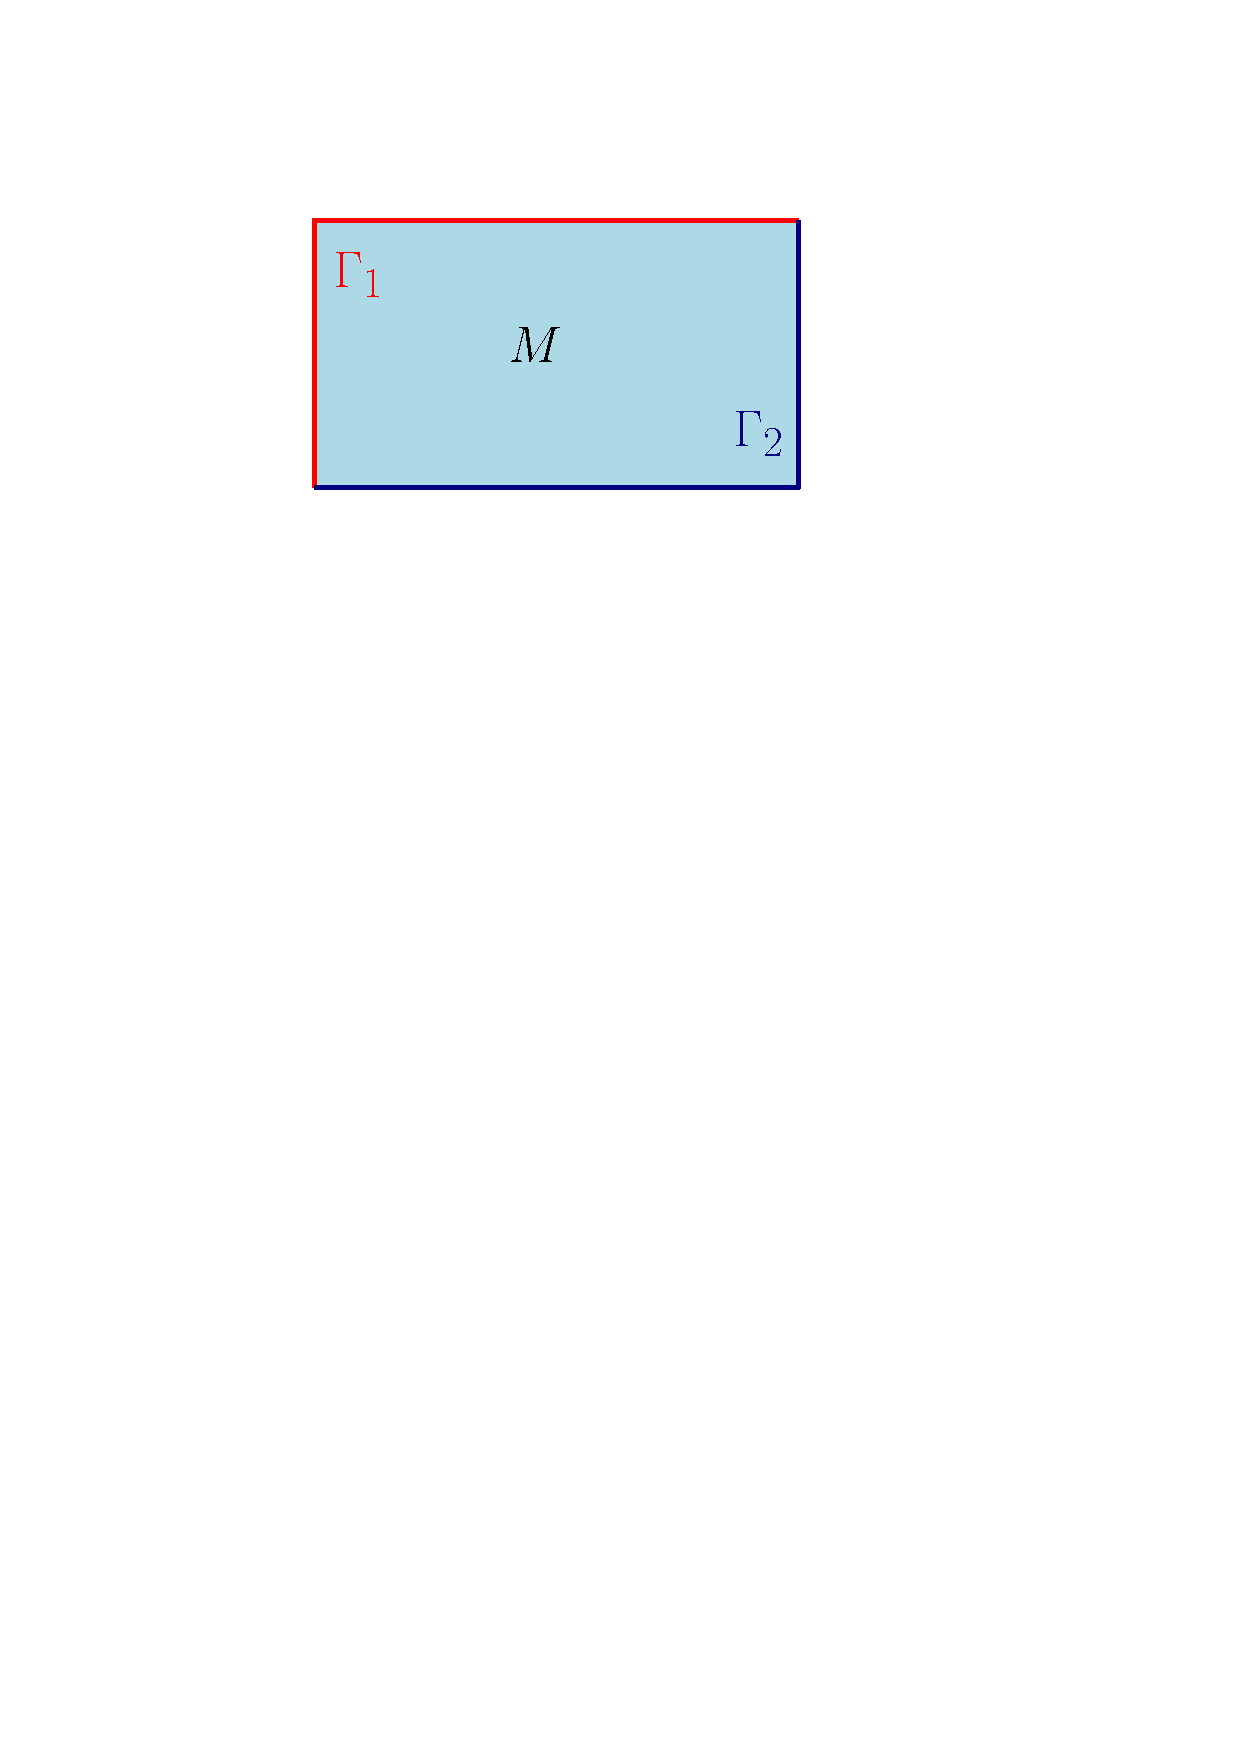
\includegraphics[width=0.46\columnwidth]{domain.pdf}}%
\hspace{8pt}%
\subfloat[][Computational mesh used for the simulation.]{%
	\label{fig:mesh}%
	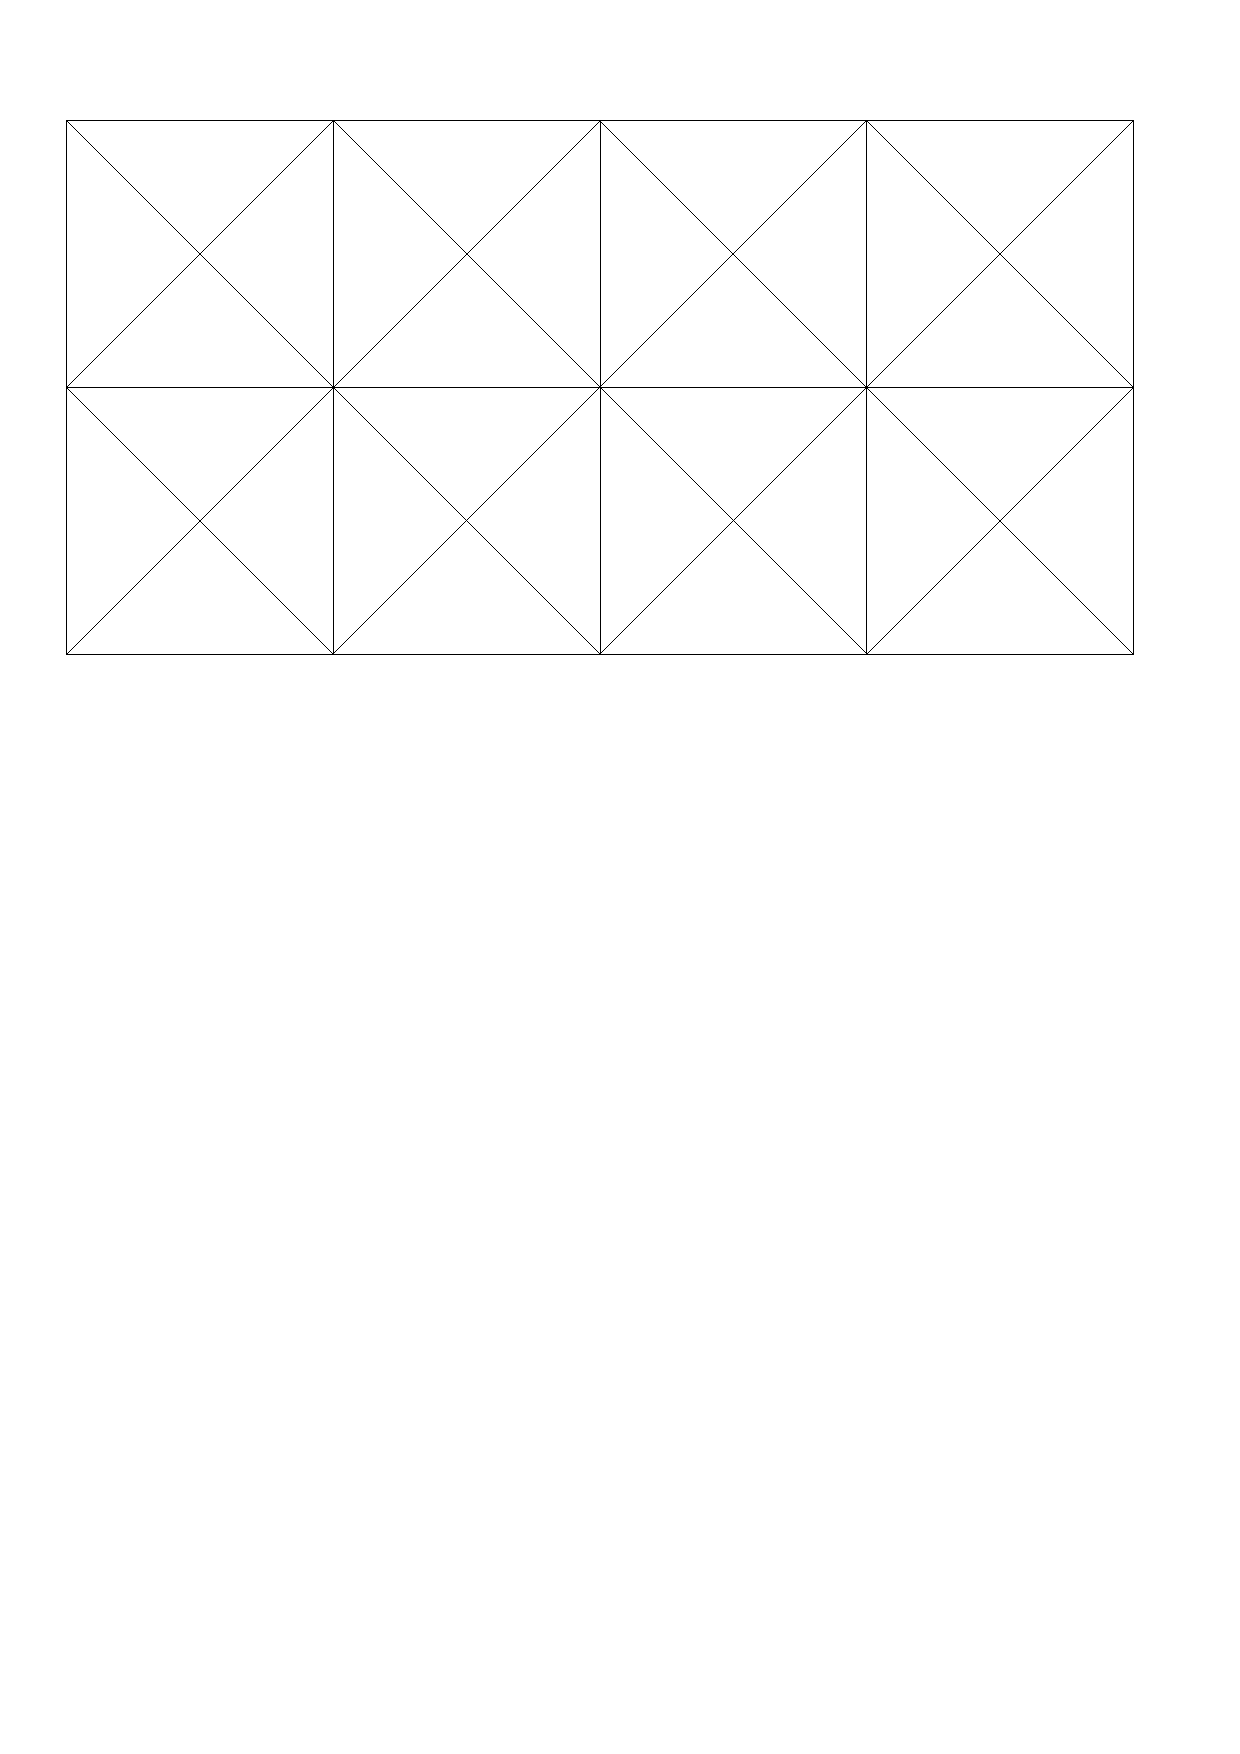
\includegraphics[width=0.51\columnwidth]{mesh.pdf}}%
\hspace{8pt}%
\subfloat[][Degrees of freedom for the 0-form.]{%
	\label{fig:zero_form}%
	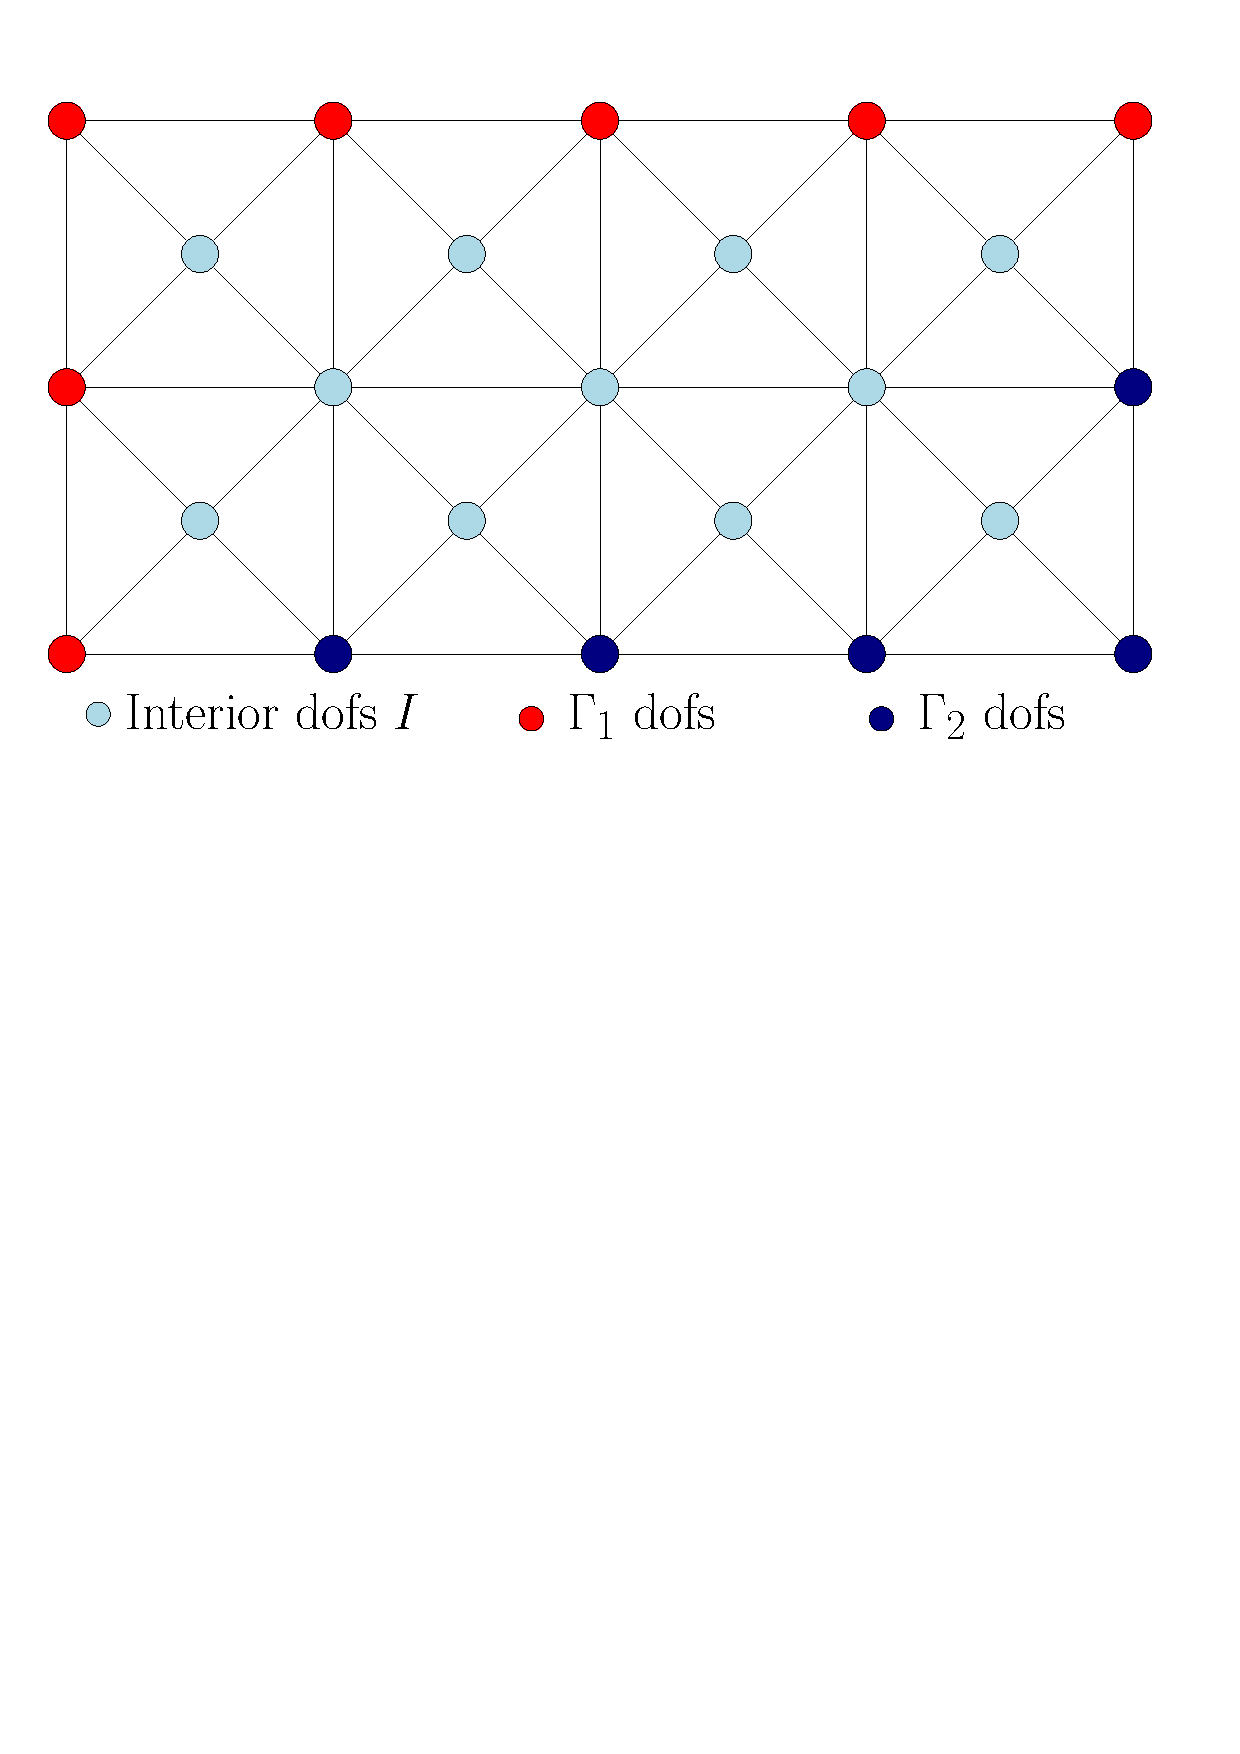
\includegraphics[width=0.48\columnwidth]{zero_form.pdf}}
	\hspace{8pt}%
\subfloat[][Degrees of freedom for the 1-form.]{%
	\label{fig:one_form}%
	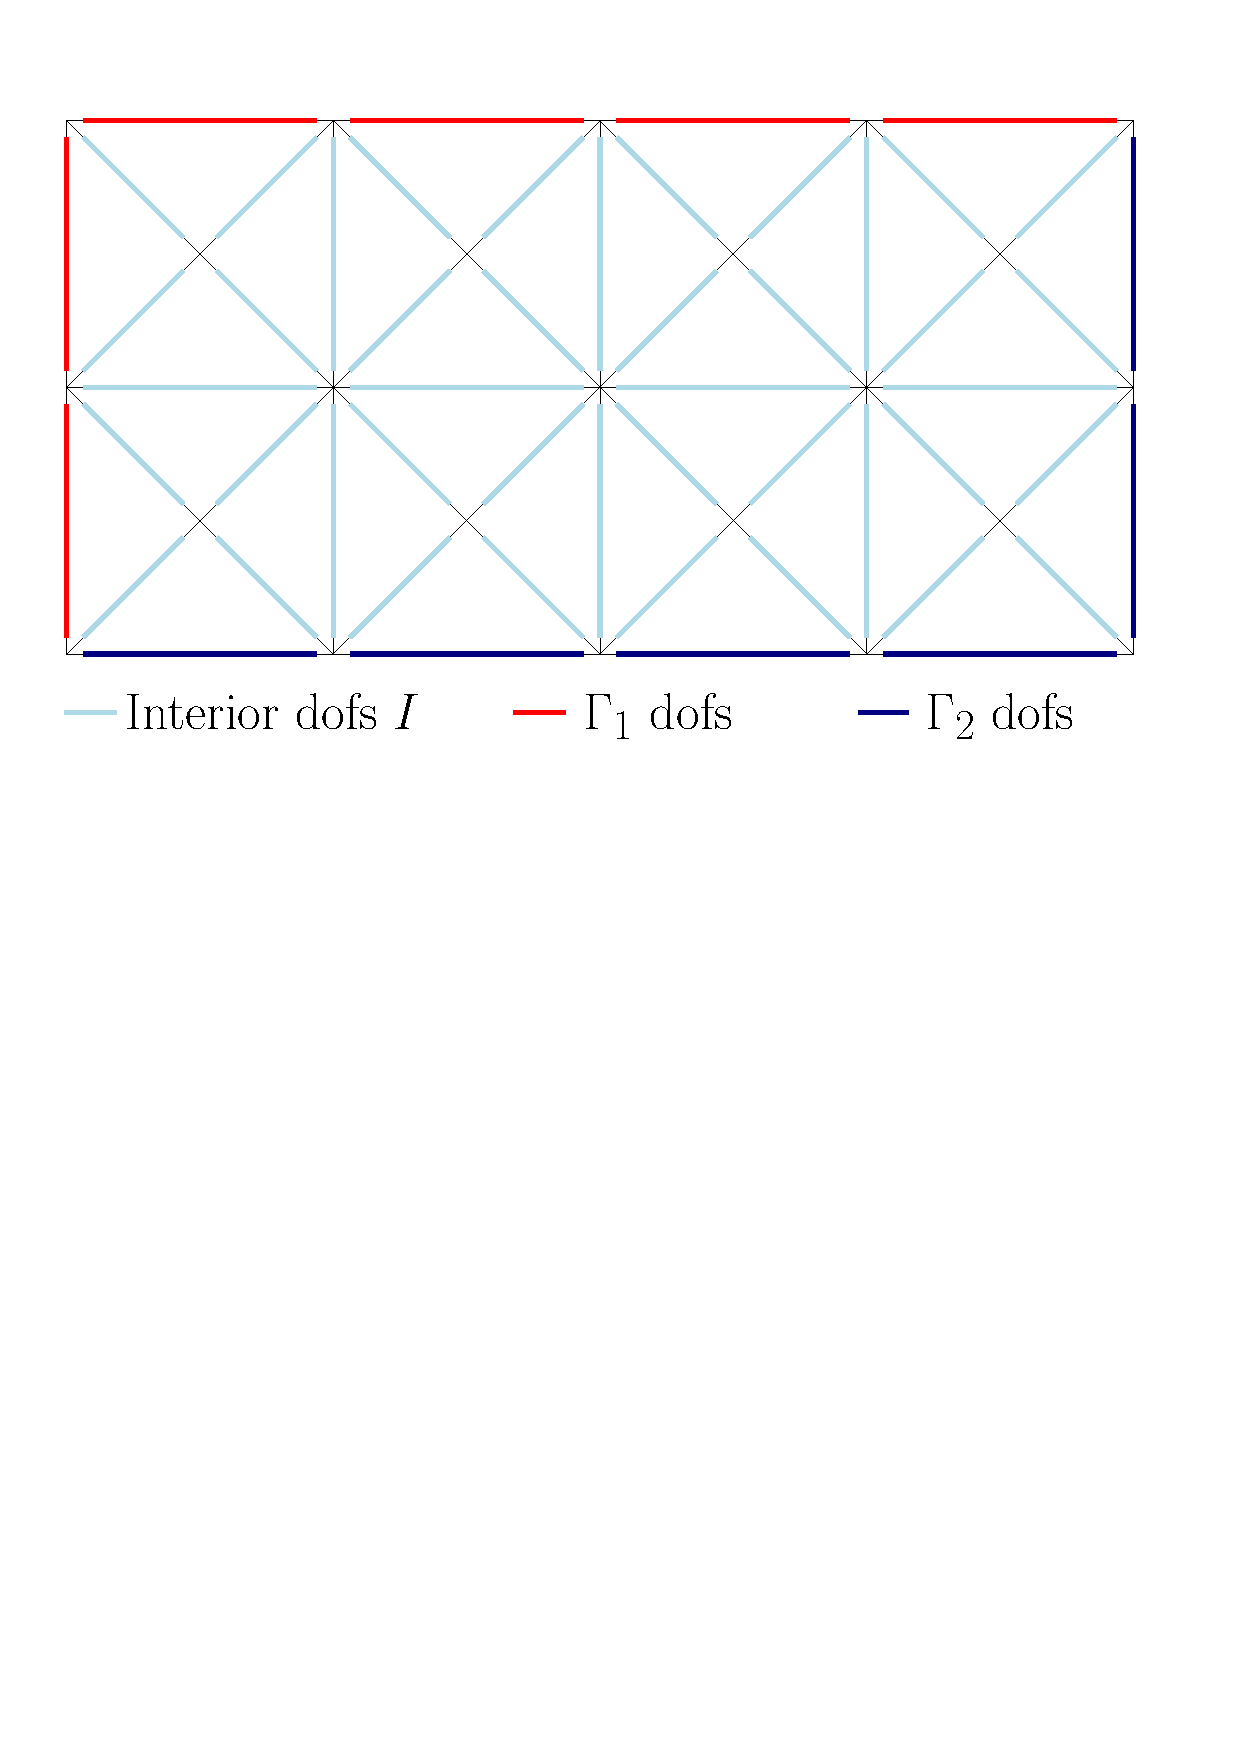
\includegraphics[width=0.46\columnwidth]{one_form.pdf}}
\caption{Example of a 2D domain with splitting of the boundary due to the boundary conditions. In the case $p=2, q=1$ the duality is between a 0-form  and a 1-form. Notice that the points at the intersection of $\Gamma_p$ and $\Gamma_q$ are attributed to $\Gamma_p$ as those will correspond to the essential boundary conditions for the 0-form.}%
\label{fig:notation_dofs}%
\end{figure}
 
Let us introduce the notation $[\mathbf{A}]_{R}^C$ (with $R, C$ index sets), that indicates the rows of matrix $\mathbf{A}$ associated with the index set $R$ and columns associated with the index set $C$, whereas the notation $[\mathbf{x}]_{R}$ indicates the vector $\mathbf{x}$ that contains elements associated with the index set $R$. Denoting by $I,\, P,\, Q$ the index sets corresponding to the interior and the subpartition ${\Gamma}_p$ and ${\Gamma}_q$ degrees of freedom respectively (cf. Fig. \ref{fig:notation_dofs}), the weak formulation \eqref{eq:weak_discr_dfPHsys} leads to the following discrete system
\begin{equation}\label{eq:discr_dfPHsys}
\begin{aligned}
    \begin{bmatrix}
        \mathbf{M}^p_{C, s} & \mathbf{0} \\
        \mathbf{0} & \mathbf{M}^q_{C, s}
    \end{bmatrix}
    \begin{pmatrix}
    \dot{\dual{\mathbf{e}}}^p \\
    \dot{\dual{\mathbf{e}}}^q
    \end{pmatrix} =&-
    \begin{bmatrix}
        \mathbf{0} & (-1)^r\mathbf{D}^{p-1}_s \\
        \mathbf{D}^{q-1}_s & \mathbf{0}
    \end{bmatrix}
    \begin{pmatrix}
    \mathbf{e}^p \\
    \mathbf{e}^q
    \end{pmatrix}, \\
    \begin{bmatrix}
        [\mathbf{M}^{q-1}_{\dual{C}, s}]_{{I}\cup Q} & \mathbf{0} \\
        \mathbf{0} & [\mathbf{M}^{p-1}_{\dual{C}, s}]_{{I}\cup P}
    \end{bmatrix}
    \begin{pmatrix}
    \dot{\mathbf{e}}^p \\
    \dot{\mathbf{e}}^q
    \end{pmatrix} = 
    &+\begin{bmatrix}
        \mathbf{0} & [(\mathbf{D}_{s}^{q-1})^\top]_{I\cup Q}\\
        (-1)^{r}[(\mathbf{D}_{s}^{p-1})^\top]_{I\cup P} & \mathbf{0}
    \end{bmatrix}
    \begin{pmatrix}
    \dual{\mathbf{e}}^p \\
    \dual{\mathbf{e}}^q
    \end{pmatrix} \\
    &+
    \begin{bmatrix}
        \mathbf{0} & (-1)^{(p-1)(q-1)}[\mathbf{B}_{s}^{p-1}]_{I\cup Q} \\
        (-1)^{p}[\mathbf{B}^{q-1}_{s}]_{I \cup P} & \mathbf{0}
    \end{bmatrix}
    \begin{pmatrix}
    {\mathbf{u}}^p \\
    {\mathbf{u}}^q
    \end{pmatrix}, \\
    \begin{pmatrix}
    \mathbf{u}^p \\
    \mathbf{u}^q \\
    \end{pmatrix} = &
    \begin{bmatrix}
    \mathbf{T}^{q-1}_{s, \Gamma_p} & \mathbf{0} \\
    \mathbf{0} & (-1)^p\mathbf{T}^{p-1}_{s, \Gamma_q} \\
    \end{bmatrix}
    \begin{pmatrix}
    \mathbf{e}^p \\
    \mathbf{e}^q
    \end{pmatrix}, 
\end{aligned}
\end{equation}
where $\mathbf{T}^k_{s, \Gamma_\circ}$ represent the restriction of the trace operator on $k$-discrete form over the boundary partition $\Gamma_\circ$ ($\circ =\{p, q\}$) and $\mathbf{B}_{s}^{p-1}, \; \mathbf{B}^{q-1}_{s}$ correspond to the boundary control matrices, defined by
\begin{equation}\label{eq:control_mat}
    \mathbf{B}^{k}_s := (\mathbf{T}^{n-k-1}_s)^\top \mathbf{\Psi}^{k}_{s, \partial}, \qquad [\mathbf{B}^{k}_s]_{ij} = \dualpr[\partial M]{\phi_{s, i}^{n-k-1}}{\psi^{k}_{s, j}}.
\end{equation}
The output degrees of freedom, defined in \eqref{eq:y}, are given by
\begin{equation}
    \begin{pmatrix}
    \mathbf{y}^p \\
    \mathbf{y}^q
    \end{pmatrix} = 
    \begin{bmatrix}
    \mathbf{T}^{q-1}_{s, \Gamma_q} & \mathbf{0}\\
    \mathbf{0} & (-1)^p \mathbf{T}^{p-1}_{s, \Gamma_p}
    \end{bmatrix}
    \begin{pmatrix}
    \mathbf{e}^p \\
    \mathbf{e}^q
    \end{pmatrix}.
\end{equation}

By definition of the trace matrices, it holds
\begin{equation}\label{eq:inout_PQ}
\begin{aligned}
    \mathbf{u}^p = \mathbf{T}^{q-1}_{s, \Gamma_p}\mathbf{e}^p = [\mathbf{e}^p]_P, \\
    \mathbf{y}^p = \mathbf{T}^{q-1}_{s, \Gamma_q}\mathbf{e}^p = [\mathbf{e}^p]_Q, 
\end{aligned}\qquad 
\begin{aligned}
    \mathbf{y}^q = (-1)^p\mathbf{T}^{p-1}_{s, \Gamma_p}\mathbf{e}^q = (-1)^p[\mathbf{e}^q]_P, \\
    \mathbf{u}^q = (-1)^p\mathbf{T}^{p-1}_{s, \Gamma_q}\mathbf{e}^q = (-1)^p[\mathbf{e}^q]_Q.
\end{aligned}
\end{equation}

\begin{remark}
The index set $P, Q$ refers to forms that lie on the boundary, i.e. of degree $p-1$ or $q-1$. The index set $P$ for variables $\mathbf{e}^p$ is different from the same index set for variable $\mathbf{e}^q$. For sake of notational lightness, we stick to this slightly abusive notation. Concerning the actual implementation, it is crucial that the index set associated for each of the boundary variables satisfy $P\cap Q = \emptyset$. 
\end{remark}

\subsubsection{Decoupling}
A very interesting property of the system \eqref{eq:discr_dfPHsys} is that it can be written as two decoupled constrained pH systems. The first system, constructed from the first and fourth line of  system \eqref{eq:discr_dfPHsys}, describes the evolution of $(\dual{e}^p,e^q)$ and is given by:
\begin{equation}\label{eq:discr_dyn_mixed14}
\begin{aligned}
    \begin{bmatrix}
        \mathbf{M}^p_{C, s} & \mathbf{0} \\
        \mathbf{0} & [\mathbf{M}^{p-1}_{\dual{C}, s}]_{I \cup P}
    \end{bmatrix}
    \begin{pmatrix}
    \dot{\dual{\mathbf{e}}}^p \\
    \dot{\mathbf{e}}^q
    \end{pmatrix} &=  (-1)^r
    \begin{bmatrix}
        \mathbf{0} & -\mathbf{D}^{p-1}_s \\
        [(\mathbf{D}_{s}^{p-1})^\top]_{I \cup P} & \mathbf{0}
    \end{bmatrix}
    \begin{pmatrix}
    \dual{\mathbf{e}}^p \\
    \mathbf{e}^q
    \end{pmatrix} +
    \begin{bmatrix}
        \mathbf{0}\\
        (-1)^{p}[\mathbf{B}^{q-1}_{s}]_{I \cup P}
    \end{bmatrix}
    \mathbf{u}^p, \\
    \mathbf{u}^q &= 
    \begin{bmatrix}
    \mathbf{0} & (-1)^p\mathbf{T}^{p-1}_{s, \Gamma_q} \\
    \end{bmatrix}
    \begin{pmatrix}
    \dual{\mathbf{e}}^p \\
    \mathbf{e}^q
    \end{pmatrix} = (-1)^p[\mathbf{e}^q]_Q,
\end{aligned}
\end{equation}

This system possesses an associated discrete Hamiltonian in terms of $(\dual{e}^p,e^q)$
\begin{equation}\label{eq:discr_H_mixed14}
H_h^{\dual{p}q} := \frac{1}{2}\inpr[M]{\dual{e}_h^p}{{C}^p \dual{e}_h^p} + \frac{1}{2}\inpr[M]{{e}_h^q}{\dual{C}^q {e}_h^q} = \frac{1}{2} (\dual{\mathbf{e}}^p)^\top \mathbf{M}^p_{C, s} \dual{\mathbf{e}}^p + \frac{1}{2} (\mathbf{e}^q)^\top \mathbf{M}^{p-1}_{\dual{C}, s} \mathbf{e}^q.
\end{equation}
 
The second system, constructed by combining the second and third line of system \eqref{eq:discr_dfPHsys}, describe the evolution of $(e^p,\dual{e}^q)$ and is given by
\begin{equation}\label{eq:discr_dyn_mixed23}
\begin{aligned}
    \begin{bmatrix}
        [\mathbf{M}^{q-1}_{\dual{C}, s}]_{I \cup Q} & \mathbf{0} \\
        \mathbf{0} & \mathbf{M}^q_{C, s}
    \end{bmatrix}
    \begin{pmatrix}
    \dot{\mathbf{e}}^p \\
    \dot{\dual{\mathbf{e}}}^q
    \end{pmatrix} &= 
    \begin{bmatrix}
        \mathbf{0} & [(\mathbf{D}_{s}^{q-1})^\top]_{I \cup Q}\\
        -\mathbf{D}^{q-1}_s & \mathbf{0}
    \end{bmatrix}
    \begin{pmatrix}
    \mathbf{e}^p \\
    \dual{\mathbf{e}}^q
    \end{pmatrix} +
    \begin{bmatrix}
        (-1)^{(p-1)(q-1)}[\mathbf{B}_{s}^{p-1}]_{I \cup Q} \\
        \mathbf{0}
    \end{bmatrix}\mathbf{u}^q, \\
    \mathbf{u}^p &= 
    \begin{bmatrix}
    \mathbf{T}^{q-1}_{s, \Gamma_p} & \mathbf{0} \\
    \end{bmatrix}
    \begin{pmatrix}
    \mathbf{e}^p \\
    \dual{\mathbf{e}}^q
    \end{pmatrix} = [\mathbf{e}^p]_P.
\end{aligned}
\end{equation}

The associated discrete Hamiltonian for this system reads
\begin{equation}\label{eq:discr_H_mixed23}
    H_h^{{p}\dual{q}} := \frac{1}{2}\inpr[M]{{e}_h^p}{\dual{C}^p {e}_h^p} + \frac{1}{2}\inpr[M]{\dual{e}_h^q}{{C}^q \dual{e}_h^q} = \frac{1}{2} ({\mathbf{e}}^p)^\top \mathbf{M}^{q-1}_{\dual{C}, s} {\mathbf{e}}^p + \frac{1}{2} (\dual{\mathbf{e}}^q)^\top \mathbf{M}^q_{C, s} \dual{\mathbf{e}}^q.  
\end{equation}


The two systems \eqref{eq:discr_dyn_mixed14} and \eqref{eq:discr_dyn_mixed23} are completely decoupled and include inhomogeneous essential boundary conditions. From a system theoretical perspective systems \eqref{eq:discr_dyn_mixed14} and \eqref{eq:discr_dyn_mixed23} are in descriptor form, i.e. they are differential-algebraic systems of index two. They correspond to pH descriptor systems, as formalized in \cite{beattie2018pHDAE}. \\

The two Hamiltonians \eqref{eq:discr_H_mixed14} and \eqref{eq:discr_H_mixed23} represent the same quantity at the continuous level and they both should (ideally) mimic the continuous power balance \eqref{eq:powbal}. However, the time derivatives of \eqref{eq:discr_H_mixed14} and \eqref{eq:discr_H_mixed23} are not the same and neither one of them mimics \eqref{eq:powbal}, as stated in the following proposition which corresponds to the modified version of Pr. \ref{pr:discr_innerpowbal} due to the strong imposition of boundary conditions.

\begin{proposition}\label{pr:discr_energyrate}
The energy rate of the Hamiltonians in Eqs. \eqref{eq:discr_H_mixed14} \eqref{eq:discr_H_mixed23} (arising from the mixed discretization) is given by  
\begin{equation}
\begin{aligned}
    \dot{H}_h^{\dual{p}q} = P_h^{\dual{p}q} := (\mathbf{u}^q)^\top \dual{\mathbf{y}}^p + (\mathbf{y}^q)^\top[\mathbf{\Psi}^{q-1}_{s, \partial}]_{P}^{P} \mathbf{u}^p, \\
    \dot{H}_h^{p\dual{q}} = P_h^{p\dual{q}} := (\mathbf{u}^p)^\top \dual{\mathbf{y}}^q + (\mathbf{u}^q)^\top[\mathbf{\Psi}^{q-1}_{s, \partial}]_{Q}^{Q} \mathbf{y}^p,
\end{aligned} 
\end{equation}
where
\begin{align}
    \dual{\mathbf{y}}^p &:= (-1)^p \{[\mathbf{M}^{p-1}_{\dual{C}, s}]_{Q} \dot{\mathbf{e}}^q  -(-1)^r[(\mathbf{D}_{s}^{p-1})^\top]_{Q} \dual{\mathbf{e}}^p\},  \label{eq:dual_yp} \\
    \dual{\mathbf{y}}^q &:= [\mathbf{M}^{q-1}_{\dual{C}, s}]_{P} \dot{\mathbf{e}}^p  -[(\mathbf{D}_{s}^{q-1})^\top]_{P} \dual{\mathbf{e}}^q, \label{eq:dual_yq}
\end{align}
\end{proposition}

\begin{proof}
For system \eqref{eq:discr_dyn_mixed14} it is obtained
\begin{equation*}
\begin{aligned}
    \dot{H}_h^{\dual{p}q} &= (\dual{\mathbf{e}}^p)^\top \mathbf{M}^p_{C, s} \dot{\dual{\mathbf{e}}}^p + (\mathbf{e}^q)^\top \mathbf{M}^{p-1}_{\dual{C}, s} \dot{\mathbf{e}}^q, \\
    &= (\dual{\mathbf{e}}^p)^\top \mathbf{M}^p_{C, s} \dot{\dual{\mathbf{e}}}^p + ([\mathbf{e}^q]_{I\cup P})^\top [\mathbf{M}^{p-1}_{\dual{C}, s}]_{I\cup P} \dot{\mathbf{e}}^q + ([\mathbf{e}^q]_{Q})^\top [\mathbf{M}^{p-1}_{\dual{C}, s}]_{Q} \dot{\mathbf{e}}^q, \\
    &= -(-1)^r ([\mathbf{e}^q]_{Q})^\top [(\mathbf{D}_{s}^{p-1})^\top]_{Q} \dual{\mathbf{e}}^p  + (-1)^{p}[\mathbf{e}^q]_{I\cup P}[\mathbf{B}^{q-1}_{s}]_{I \cup P} \mathbf{u}^p + ([\mathbf{e}^q]_{Q})^\top [\mathbf{M}^{p-1}_{\dual{C}, s}]_{Q} \dot{\mathbf{e}}^q, \\
    &= (-1)^p(\mathbf{u}^q)^\top \{[\mathbf{M}^{p-1}_{\dual{C}, s}]_{Q} \dot{\mathbf{e}}^q  -(-1)^r[(\mathbf{D}_{s}^{p-1})^\top]_{Q} \dual{\mathbf{e}}^p\} + (\mathbf{y}^q)^\top[\mathbf{\Psi}^{q-1}_{s, \partial}]_{P}^{P} \mathbf{u}^p. 
\end{aligned}
\end{equation*}
Notice that the matrix $[\mathbf{\Psi}^{q-1}_{s}]_{P}^{P}$ is rectangular. Similarly, for system \eqref{eq:discr_dyn_mixed23}, it is obtained
\begin{equation*}
\begin{aligned}
    \dot{H}_h^{p\dual{q}} &= ({\mathbf{e}}^p)^\top \mathbf{M}^{q-1}_{\dual{C}, s} \dot{\mathbf{e}}^p + (\dual{\mathbf{e}}^q)^\top \mathbf{M}^q_{C, s} \dot{\dual{\mathbf{e}}}^q, \\  
    &=([{\mathbf{e}}^p]_{I\cup Q})^\top [\mathbf{M}^{q-1}_{\dual{C}, s}]_{I\cup Q} \dot{\mathbf{e}}^p + ([{\mathbf{e}}^p]_{P})^\top [\mathbf{M}^{q-1}_{\dual{C}, s}]_{P} \dot{\mathbf{e}}^p + (\dual{\mathbf{e}}^q)^\top \mathbf{M}^q_{C, s} \dot{\dual{\mathbf{e}}}^q,\\
    &=- \mathbf{e}^p[(\mathbf{D}_{s}^{q-1})^\top]_{P}\dual{\mathbf{e}}^q  + (-1)^{(p-1)(q-1)} \mathbf{e}^p [\mathbf{B}_{s}^{p-1}]_{I \cup Q} \mathbf{u}^q +  ([{\mathbf{e}}^p]_{P})^\top [\mathbf{M}^{q-1}_{\dual{C}, s}]_{P} \dot{\mathbf{e}}^p,\\
    &=(\mathbf{u}^p)^\top \{[\mathbf{M}^{q-1}_{\dual{C}, s}]_{P} \dot{\mathbf{e}}^p  -[(\mathbf{D}_{s}^{q-1})^\top]_{P} \dual{\mathbf{e}}^q\} + (\mathbf{u}^q)^\top[\mathbf{\Psi}^{q-1}_{s, \partial}]_{Q}^{Q} \mathbf{y}^p.
\end{aligned}
\end{equation*}
Given definitions \eqref{eq:dual_yp}, \eqref{eq:dual_yq}, the statement is proven. 
\end{proof}

In conclusion, for the case of uniform boundary conditions it is sufficient to consider only one of the two mixed discretization Eqs. \eqref{eq:discr_dyn_mixed14} and \eqref{eq:discr_dyn_mixed23} to obtain the preservation of the discrete power balance (as in the Partitioned Finite Element method \cite{cardoso2020pfem}). For example in the case in which $\Gamma_p =\partial M, \; \Gamma_q = \emptyset$, then the energy rate reads
\begin{equation}
    \dot{H}_h^{\dual{p}q}= (\mathbf{y}^q)^\top\mathbf{\Psi}^{q-1}_{s, \partial} \mathbf{u}^p.
\end{equation}
Conversely, if $\Gamma_p =\emptyset, \; \Gamma_q = \partial M$, then the energy rate reads
\begin{equation}
    \dot{H}_h^{p\dual{q}} = (\mathbf{u}^q)^\top\mathbf{\Psi}^{q-1}_{s, \partial} \mathbf{y}^p.
\end{equation}
However, in this general case of mixed boundary conditions, both systems are needed in order to recover a discrete Stokes-Dirac structure and its associated power balance, as will be shown next.


\subsubsection{Recovering the power balance}
The continuous power balance \eqref{eq:H_dot} written in the terms of efforts can be expressed as
\begin{equation}
    P = \dualpr[M]{e^p}{C^p\partial_t \dual{e}^p} + \dualpr[M]{e^q}{C^q\partial_t \dual{e}^q}.
\end{equation}
Its discrete version is then given by 
\begin{equation}
    P_h = \dualpr[M]{e^p_h}{C^p\partial_t \dual{e}^p_h} + \dualpr[M]{e^q_h}{C^q\partial_t \dual{e}^q_h} = \mathbf{e}^p \mathbf{L}_{C,s}^p \dot{\dual{\mathbf{e}}}^p + \mathbf{e}^q \mathbf{L}_{C,s}^q \dot{\dual{\mathbf{e}}}^q.
\end{equation}
where $[\mathbf{L}_{C, s}^k]_{ij} := \dualpr[M]{\phi^{n-k}_{s, i}}{C^k \phi^k_{s, j}}$. The dual field formulation is such to preserve the power balance at the discrete level, under some regularity assumption for the physical coefficients. This is due to the fact that each mixed system \eqref{eq:discr_dyn_mixed14} and \eqref{eq:discr_dyn_mixed23} contains an equation (the one belonging to the Stokes-Dirac structure) that is strongly verified, leading to a discrete conservation law.

\begin{proposition}\label{pr:discr_Hdot}
If the tensors $C^p, \; C^q$ verify the following regularity assumption
\begin{equation}\label{eq:reg_C}
    C^p: H\Omega^p(M) \rightarrow H\Omega^p(M), \qquad C^q: H\Omega^q(M) \rightarrow H\Omega^q(M),
\end{equation}
then the discrete power satisfies
\begin{equation}
    P_h = \dualpr[\partial M]{e^\partial_h}{f^\partial_h} = \mathbf{e}^\partial \mathbf{\Psi}^{q-1}_{s, \partial} \mathbf{f}^\partial.
\end{equation}
\end{proposition}

\begin{proof}
Since the tensors satisfy the regularity assumption, the subcomplex property (Th. \ref{th:fe_subcomplex}) to the first line of \eqref{eq:discr_dyn_mixed14} and the second line of \eqref{eq:discr_dyn_mixed23} provides
\begin{equation*}
C^p\partial_t\dual{e}^p_h = -(-1)^r\d e^q_h, \qquad C^q\partial_t\dual{e}^q_h = -\d e^p_h.
\end{equation*}
Taking the duality product against $e^p_h$ and $e_h^q$ provides
\begin{equation*}
P_h= -\dualpr[M]{e^p_h}{(-1)^r\d e^q_h}-\dualpr[M]{e_h^q}{\d e^p_h}.
\end{equation*}
The application of the Stokes Theorem then gives
\begin{equation*}
P_h = \dualpr[\partial M]{(-1)^p e^q_h}{e^p_h}= \dualpr[\partial M]{e^\partial_h}{f^\partial_h},
\end{equation*}
leading to the proof of the statement.
\end{proof}

If the physical coefficients are not regular, the power balance can be preserved but the constitutive equations need to be kept separated from the dynamics. 


\section{Time discretization}\label{sec:time_discr}

To ensure discrete conservation of energy, implicit Runge-Kutta methods based on Gauss-Legendre collocation points can be used \cite{sanzserna1992}. These methods are also the only collocation schemes that lead to an exact discrete energy balance in the linear case \cite{kotyczka2019discrete}. The implicit midpoint method is here used to illustrate the time discretization. \\

Consider a total simulation time $T_{\mathrm{end}}$ and a equidistant splitting given by the time step $\Delta t = T_{\mathrm{end}}/N_t$, where $N_t$ is the total number of simulation instants. The evaluation of a generic variable $\mathbf{x}$ at the time instant $t_n = n\Delta t$ is denoted by $\mathbf{x}_n$. The midpoint method is the simplest method in the class of collocation methods known as Gauss-Legendre methods. It applies to systems of the form
\begin{equation}
    \dot{\mathbf{x}} = \mathbf{f}(\mathbf{x}, t), \qquad \mathbf{x} \in \bbR^d, \qquad \mathbf{f}: \bbR^{d} \rightarrow \bbR^d.
\end{equation}
This method is a one stage method, i.e. only uses the information at the previous time, and seeks for the solution of the implicit equation
\begin{equation}
    \mathbf{x}_{n+1} = \mathbf{x}_{n} + \Delta t \; \mathbf{f}\left(\mathbf{x}_{n+1/2},  t_{n+1/2}\right),
\end{equation}
where $\mathbf{x}_{n+1/2}:= \frac{\mathbf{x}_{n+1} + \mathbf{x}_{n}}{2}$ and $t_{n+1/2}:= t_n + \frac{\Delta t}{2}$. The application of the implicit midpoint method to system \eqref{eq:discr_dyn_mixed14} with direct assignment of the boundary degrees of freedom leads to the algebraic system
\begin{equation}\label{eq:timediscr_14}
    \mathbf{A}^{\dual{p}q}_{\mathrm{bc}}
    \begin{pmatrix}
    \dual{\mathbf{e}}^p_{n+1} \\ [\mathbf{e}^q_{n+1}]_{I\cup P}
    \end{pmatrix}
    = \mathbf{b}^{\dual{p}q}_{\mathrm{bc}}.
\end{equation}
The matrix $\mathbf{A}^{\dual{p}q}_{\mathrm{bc}}$ corresponds to 
\begin{equation}
\mathbf{A}^{\dual{p}q}_{\mathrm{bc}} =
    \begin{bmatrix}
        \mathbf{M}^p_{C, s} & \frac{1}{2}(-1)^r\Delta t [\mathbf{D}^{p-1}_s]^{I\cup P} \\
        -\frac{1}{2}(-1)^r\Delta t [(\mathbf{D}_{s}^{p-1})^\top]_{I\cup P} & [\mathbf{M}^{p-1}_{\dual{C}, s}]_{I\cup P}^{I\cup P}
    \end{bmatrix}.
\end{equation}
The $\mathbf{b}^{\dual{p}q}_{\mathrm{bc}}$ vector incorporates the forcing due to the previous time step and the boundary conditions
\begin{equation}
\begin{aligned}
\mathbf{b}^{\dual{p}q}_{\mathrm{bc}} = \begin{bmatrix}
        \mathbf{M}^p_{C, s} & -\frac{1}{2}(-1)^r\Delta t[\mathbf{D}^{p-1}_s]^{I\cup P} \\
        \frac{1}{2}(-1)^r\Delta t [(\mathbf{D}_{s}^{p-1})^\top]_{I\cup P} & [\mathbf{M}^{p-1}_{\dual{C}, s}]_{I\cup P}^{I\cup P}
    \end{bmatrix}\begin{pmatrix}
    \dual{\mathbf{e}}^p_n \\
    [\mathbf{e}^q_n]_{I\cup P}
    \end{pmatrix} \\
    - (-1)^p
    \begin{bmatrix}
         \mathbf{0} \\
        [\mathbf{M}^{p-1}_{\dual{C}, s}]_{I\cup P}^{Q}
    \end{bmatrix}(\mathbf{u}^q_{n+1} - \mathbf{u}^q_{n}) 
    + (-1)^p\Delta t \begin{bmatrix}
        -(-1)^r [\mathbf{D}^{p-1}_s]^{Q} & \mathbf{0}\\
        \mathbf{0} & [\mathbf{B}^{q-1}_{s}]_{I \cup P}
    \end{bmatrix}
    \begin{pmatrix}
        \mathbf{u}^q_{n+1/2} \\
        \mathbf{u}^p_{n+1/2}
    \end{pmatrix}.
\end{aligned}
\end{equation}

The implicit midpoint method, once applied to \eqref{eq:discr_dyn_mixed23}, leads to the system
\begin{equation}\label{eq:timediscr_23}
    \mathbf{A}^{p\dual{q}}_{\mathrm{bc}}
    \begin{pmatrix}
    [\mathbf{e}^p_{n+1}]_{I\cup Q} \\ \dual{\mathbf{e}}^q_{n+1}
    \end{pmatrix}
    = \mathbf{b}^{p\dual{q}}_{\mathrm{bc}},
\end{equation}
with
\begin{equation}
\mathbf{A}^{p\dual{q}}_{\mathrm{bc}} =
    \begin{bmatrix}
        [\mathbf{M}^{q-1}_{\dual{C}, s}]^{I\cup Q}_{I\cup Q} & -\frac{1}{2}\Delta t [(\mathbf{D}^{q-1}_s)^\top]_{I\cup Q} \\
        \frac{1}{2}\Delta t [\mathbf{D}_{s}^{q-1}]^{I\cup Q} & \mathbf{M}^{q}_{{C}, s}
    \end{bmatrix}
\end{equation}
and 
\begin{equation}
\begin{aligned}
\mathbf{b}^{p\dual{q}}_{\mathrm{bc}} = 
\begin{bmatrix}
        [\mathbf{M}^{q-1}_{\dual{C}, s}]^{I\cup Q}_{I\cup Q} & \frac{1}{2}\Delta t [(\mathbf{D}^{q-1}_s)^\top]_{I\cup Q} \\
        -\frac{1}{2}\Delta t [\mathbf{D}_{s}^{q-1}]^{I\cup Q} & \mathbf{M}^{q}_{{C}, s}
\end{bmatrix}
    \begin{pmatrix}
    [\mathbf{e}^p_{n}]_{I\cup Q} \\ \dual{\mathbf{e}}^q_{n}
    \end{pmatrix} \\
    -
    \begin{bmatrix}
        [\mathbf{M}^{q-1}_{\dual{C}, s}]_{I\cup Q}^{P} \\
        \mathbf{0} \\
    \end{bmatrix}(\mathbf{u}^p_{n+1} - \mathbf{u}^p_{n}) 
    + \Delta t \begin{bmatrix}
        \mathbf{0} & (-1)^{(p-1)(q-1)}[\mathbf{B}^{p-1}_{s}]_{I \cup Q} \\
        -[\mathbf{D}^{q-1}_s]^{P} & \mathbf{0}\\
    \end{bmatrix}
    \begin{pmatrix}
        \mathbf{u}^p_{n+1/2} \\
        \mathbf{u}^q_{n+1/2}
    \end{pmatrix}.
\end{aligned}
\end{equation}

\begin{proposition}\label{pr:discrtime_energyrate}
Given the recursions implemented by systems \eqref{eq:timediscr_14} and \eqref{eq:timediscr_23}, the following time discrete energy rate holds
\begin{equation}
\begin{aligned}
    \frac{H^{\dual{p}q}_{h, n+1} - H^{\dual{p}q}_{h, n}}{\Delta t} &= P_{h, n+1/2}^{\dual{p}q} := (\mathbf{u}^q_{n+1/2})^\top \dual{\mathbf{y}}^p_{n+1/2} +  (\mathbf{y}^q_{n+1/2})^\top [\mathbf{\Psi}^{q-1}_{s}]_{P}^{P} \mathbf{u}^p_{n+1/2}, \\
    \frac{H^{p\dual{q}}_{h, n+1} - H^{p\dual{q}}_{h, n}}{\Delta t} 
    &= P_{h, n+1/2}^{p\dual{q}} := (\mathbf{u}^p_{n+1/2})^\top \dual{\mathbf{y}}^q_{n+1/2} +  (\mathbf{u}^q_{n+1/2})^\top [\mathbf{\Psi}^{q-1}_{s}]_{Q}^{Q} \mathbf{y}^p_{n+1/2},
\end{aligned}
\end{equation}
where $\dual{\mathbf{y}}^p_{n+1/2}$ and $\dual{\mathbf{y}}^q_{n+1/2}$ correspond a midpoint discretization of Eqs. \eqref{eq:dual_yp} and \eqref{eq:dual_yq} respectively
\begin{equation}
\begin{aligned}
\dual{\mathbf{y}}^p_{n+1/2} &:= (-1)^p \left\{[\mathbf{M}^{p-1}_{\dual{C}, s}]_{Q} \frac{\mathbf{e}^q_{n+1}-\mathbf{e}^q_{n}}{\Delta t}  -(-1)^r[(\mathbf{D}_{s}^{p-1})^\top]_{Q} \dual{\mathbf{e}}^p_{n+1/2}\right\}, \\
\dual{\mathbf{y}}^q_{n+1/2} &:= [\mathbf{M}^{q-1}_{\dual{C}, s}]_{P} \frac{\mathbf{e}^p_{n+1} - \mathbf{e}^p_{n}}{\Delta t} -[(\mathbf{D}_{s}^{q-1})^\top]_{P} \dual{\mathbf{e}}^q_{n+1/2}.
\end{aligned}
\end{equation}
\end{proposition}
\begin{proof}
The time discrete energy rates are obtained by vector multiplication of Systems \eqref{eq:timediscr_14} and \eqref{eq:timediscr_23} by $\begin{pmatrix}
    \dual{\mathbf{e}}^p_{n+1/2} \\ [\mathbf{e}^q_{n+1/2}]_{I\cup P}
\end{pmatrix}$ and $\begin{pmatrix}
    [\mathbf{e}^p_{n+1/2}]_{I\cup Q} \\ \dual{\mathbf{e}}^q_{n+1/2}
    \end{pmatrix}$ respectively. This computation provides the implicit midpoint discretization of Proposition \ref{pr:discr_energyrate}.
\end{proof}

The algebraic systems \eqref{eq:timediscr_14} and \eqref{eq:timediscr_23} satisfy a time discrete power balance, together with time discrete energy rates.
\begin{proposition}\label{pr:discrtime_Hdot}
Given the recursions implemented by systems \eqref{eq:timediscr_14} and \eqref{eq:timediscr_23}, the regularity assumption reported in Eq. \eqref{eq:reg_C}, and the following definition of time discrete power
\begin{equation*}
    P_{h, n+1/2} := \frac{1}{\Delta t}\dualpr[M]{e^p_{h, n+1/2}}{C^p (\dual{e}^p_{h, n+1}- \dual{e}^p_{h, n})} + \frac{1}{\Delta t}\dualpr[M]{e^q_{h, n+1/2}}{C^q (\dual{e}^q_{h, n+1}-\dual{e}^q_{h, n})},
\end{equation*}
it holds
\begin{equation}
    P_{h, n+1/2} = (\mathbf{e}^\partial_{n+1/2})^\top \mathbf{\Psi}^{q-1}_{s, \partial}\mathbf{f}^\partial_{n+1/2}.
\end{equation}
\end{proposition}
\begin{proof}
The time discrete power balance corresponds to the implicit midpoint time discretization of Proposition \ref{pr:discr_Hdot}.
\end{proof}

\section{Numerical experiments}\label{sec:num_exp}

In this section, the dual field discretization methodology proposed in this work is tested for the wave and Maxwell equations in a box-shaped three-dimensional domain
$$M = \{ (x,y,z) \in [0, 1]\times[0, 1/2]\times[0, 1/2] \}.$$ 
The boundary sub-partitions are selected to be
\begin{equation*}
    \Gamma_p = \{(x,y,z) \vert \; x=0 \cup y=0 \cup z=0\}, \qquad \Gamma_q = \{(x, y, z) \vert \; x=1 \cup y=1/2 \cup z=1/2 \}.
\end{equation*}

Since we want to rely on existing and well-established librairies like \fenics and \firedrake, the equations need to be translate into vector calculus operations. By introducing the musical isomorphism, given by the flat $\flat$ and the sharp operator $\sharp$ (cf. \ref{app:vec_ext}), and the isomorphism $\beta$ converting vector fields in $n-1$ forms, the commuting diagram in Fig. \ref{fig:cd_ext_vec}, that provides the link between the de Rham complex and the standard operators and Sobolev space from vector calculus, is obtained.
\begin{figure}[h]
\centering
\begin{tikzcd}
H\Omega^0(M) \arrow[r, "\d"] \arrow[d, leftrightarrow, "Id"]
& H\Omega^{1}(M) \arrow[r, "\d"] \arrow[d, "\sharp", xshift=10pt] & H\Omega^2(M) \arrow[r, "\d"] \arrow[d, "\beta^{-1}", xshift=10pt]
& H\Omega^{3}(M) \arrow[d, "\star", xshift=10pt]  \\
H^1(M) \arrow[r, "\grad"]
& H^{\curl}(M) \arrow[r, "\curl"] \arrow[u, "\flat"] & H^{\div}(M) \arrow[r, "\div"] \arrow[u, "\beta"]
& L^2(M) \arrow[u, "\star^{-1}"]
\end{tikzcd}  
\caption{Equivalence of vector and exterior calculus Sobolev spaces.}
\label{fig:cd_ext_vec}
\end{figure}

Since the manifold is a subset of the Euclidean space, the metric tensor is the identity $g_{ij}~=~\delta_{ij}$. The finite element arising from the trimmed polynomial family on the computational mesh $\mathcal{T}_h$ are then equivalent to the well known continuous Galerkin (or Lagrange) elements $\mathcal{P}^-_s\Omega^0(\mathcal{T}_h) \equiv \mathrm{CG}_s(\mathcal{T}_h)$, Nédélec of the first kind $\mathcal{P}^-_s\Omega^1(\mathcal{T}_h) \equiv \mathrm{NED}_s^1(\mathcal{T}_h)$, Raviart-Thomas $\mathcal{P}^-_s\Omega^2(\mathcal{T}_h) \equiv \mathrm{RT}_s(\mathcal{T}_h)$ and discontinuous Galerkin $\mathcal{P}^-_s\Omega^3(\mathcal{T}_h) \equiv \mathrm{DG}_{s-1}(\mathcal{T}_h)$, as illustrated in  diagram \ref{fig:fe_ext_vec}.

\begin{figure}[h]
\centering
\begin{tikzcd}
H^1(M) \arrow[r, "\grad"] \arrow[d, "\Pi_{s, h}^{-, 0}"]
& H^{\curl}(M) \arrow[r, "\curl"] \arrow[d, "\Pi_{s, h}^{-, 1}"] & H^{\div}(M) \arrow[r, "\div"] \arrow[d, "\Pi_{s, h}^{-, 2}"]
& L^2(M) \arrow[d, "\Pi_{s, h}^{-, 3}"]  \\
\mathrm{CG}_s(\mathcal{T}_h) \arrow[r, "\grad"] 
& \mathrm{NED}_s^1(\mathcal{T}_h) \arrow[r, "\curl"] & \mathrm{RT}_s(\mathcal{T}_h) \arrow[r, "\div"]
& \mathrm{DG}_{s-1}(\mathcal{T}_h) 
\end{tikzcd}  
\caption{Equivalence between finite element differential forms and classical elements.}
\label{fig:fe_ext_vec}
\end{figure}

The finite element library \firedrake \cite{rathgeber2017firedrake} is used for the numerical investigation.

\begin{remark}
As argued in \cite{benner2015timebc}, the method of manufactured solution is not suited for boundary control problems. This is due to the fact that for finer dsicretizations the volume terms due to the forcing will dominate over the boundary terms. This is the reason why the numerical tests are set up considering an eigensolution rather than a manufactured one induced by a forcing.
\end{remark}

\subsection{The acoustic wave equation in $3D$}

The acoustic wave equation corresponds to the case $p=3$ and $q=1$. The energy variables are the top-form $p^3:=\alpha^p$ (corresponding to the pressure) and the one-form $q^1:=\alpha^q$ (corresponding to the linear momentum). If the physical coefficients are normalized to one (this can be easily achieved by re-scaling the time with respect to the speed of sound), the Hamiltonian is given by
\begin{equation}
    H(p^3, q^1) = \frac{1}{2} \int_M p^3 \wedge \star p^3 + q^1 \wedge \star q^1,
\end{equation}
with its variational derivatives given by
\begin{equation}
p^0:=\delta_{p^3} H = \star p^3, \qquad  q^2:= \delta_{q^1} H = \star q^1  ,  
\end{equation}
leading to the pH system
\begin{equation}\label{eq:wave_eq}
    \begin{pmatrix}
    \partial_t p^3 \\
    \partial_t q^1
    \end{pmatrix} =
    -
    \begin{bmatrix}
    0 & \d^2 \\
    \d^0 & 0 \\
    \end{bmatrix}
    \begin{pmatrix}
    p^0 \\
    q^2
    \end{pmatrix}, \qquad 
    \begin{aligned}
    \tr p^0 \vert_{\Gamma_p} &= u^p, \\
    -\tr q^2 \vert_{\Gamma_q} &= u^q.
 \end{aligned}
\end{equation}

Given the functions
\begin{equation}
    g(x, y, z) = \cos(x) \sin(y) \sin(z), \qquad f(t) = 2 \sin(\sqrt{3} t) + 3 \cos(\sqrt{3} t),
\end{equation}
an exact solution of \eqref{eq:wave_eq} is given by
%the system  is identically solved by
\begin{equation}\label{eq:wave_exsol}
\begin{aligned}
p^3_{\mathrm{ex}} &= \star g \diff{f}{t}, \\    
q^1_{\mathrm{ex}} &= -\d{g} f, 
\end{aligned} \qquad 
\begin{aligned}
p^0_{\mathrm{ex}} &= g \diff{f}{t}, \\
q^2_{\mathrm{ex}} &= -\star \d{g} f,
\end{aligned}
\end{equation}
The exact solution provides the appropriate inputs to be fed into the system
\begin{equation}
    u^p = \left. \tr p^0_{\mathrm{ex}} \right\vert_{\Gamma_p}, \qquad u^q =  -\tr q^2_{\mathrm{ex}} \vert_{\Gamma_q}.
\end{equation}

The employment of the dual field discretization leads to the resolution of 4 equation in the unknowns $p^3, \; q^1$ (the primal variables, coinciding with the dual efforts) $p^0, \; q^2$ (the dual variables, coinciding with the efforts). Each variables is discretized using the associated finite element differential forms:
\begin{itemize}
    \item discontinuous Galerkin elements DG$_{s-1}$ for $p^3_h$;
    \item Nédélec elements of the first kind NED$_s^1$ for $q^1_h$;
    \item continuous Galerkin elements CG$_s$ for $p^0_h$;
    \item Raviart Thomas elements RT$_s$ for $q^2_h$.
\end{itemize}


\subsubsection{Energy Conservation properties}
First the conservation properties of the scheme are verified against the exact solution \eqref{eq:wave_exsol}. The test is performed using $N_{\text{el}}=4$ elements for each side of the box-shaped domain and polynomial degree $s=3$. Concerning the time discretization, the total simulation time $T_{\text{end}}=5$ and the time step is taken to be $\Delta t= \frac{T_{\text{end}}}{200}$. \\

The energy rate conservation, expected by Prop. \ref{pr:discrtime_energyrate}, is reported in Fig. \ref{fig:con_Hdot_wave}. Fig. \ref{fig:con_P_wave} shows the fulfilment of the discrete power balance (Prop. \ref{pr:discrtime_Hdot}), whereas Fig. \ref{fig:err_flow_wave} provides the error between the discrete and exact power flow. The power flow error due to the polynomial interpolation is lower than $10^{-4}$. 
For what concerns the energy behaviour, three different energies are considered
\begin{equation*}
\begin{aligned}
    H^{\widehat{3}1}_h&= \frac{1}{2} \int_M p^3_h \wedge \star p^3_h + q^2_h \wedge \star q_h^2, \\
    H^{3\widehat{1}}_h&= \frac{1}{2} \int_M p^0_h \wedge \star p^0_h + q^1_h \wedge \star q_h^1, \\
    \frac{H_T}{2} &= \frac{1}{2} \int_M p^0_h \wedge p^3_h + q^2_h \wedge q_h^1. \\
\end{aligned}
\end{equation*}
The first two energies are associated with the mixed discretization \eqref{eq:discr_dyn_mixed14}, \eqref{eq:discr_dyn_mixed23}, whereas the last one is constructed using the dual field formulation. The errors on the energy rate and variation of energy, shown in Fig. \ref{fig:energy_wave}, are of the order $10^{-5}$, assessing the performance of the dual field formulation. In particular, one can notice that the energy $\frac{H_T}{2}$ stays between $H^{\widehat{3}1}_h, \; H^{3\widehat{1}}_h$ at all times. The variation of energy is also computed using the power flow 
\begin{equation*}
    \Delta H = \int_0^t P_h(\tau) \d\tau, \qquad P_h = \int_M p^0_h \wedge \partial_t p^3_h + q^2_h \wedge \partial_t q_h^1.
\end{equation*}
As shown in Fig. \ref{fig:deltaH_wave} this quantity is less affected by the error for this particular test case. 



\begin{figure}[p]%
\centering
\subfloat[][Conservation law for $\dot{H}^{\widehat{3}1}_h - P_h^{\widehat{3}1}$]{%
	\label{fig:con_H32_wave}%
	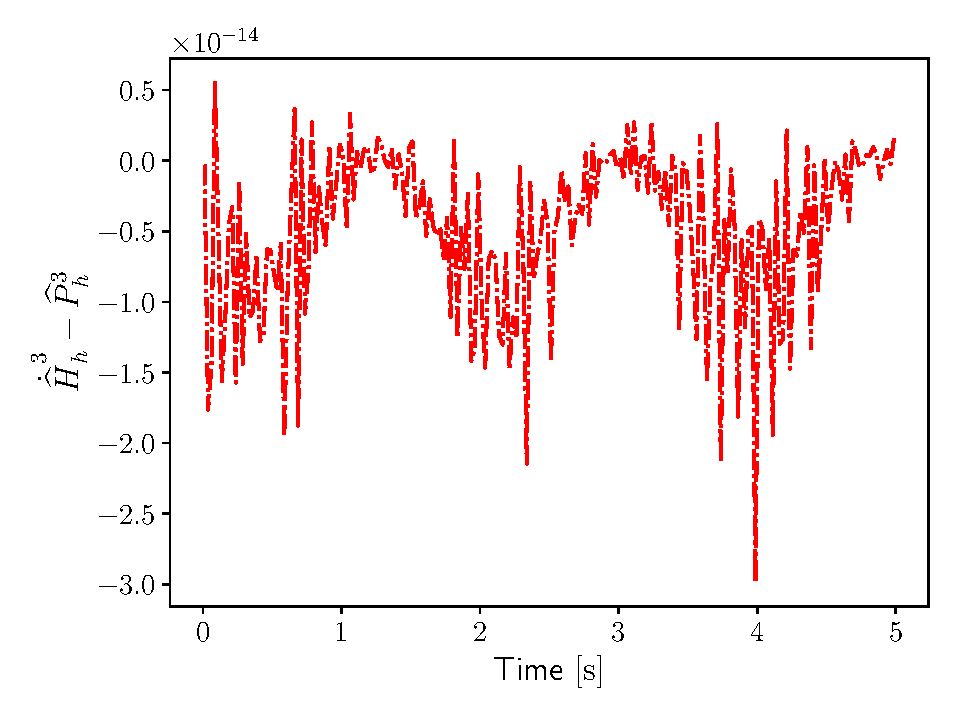
\includegraphics[width=0.48\columnwidth]{pow_bal32_3D_DN.pdf}}%
\hspace{8pt}%
\subfloat[][Conservation law for $\dot{H}^{3\widehat{1}}_h-P^{3\widehat{1}}_h$]{%
	\label{fig:con_H10_wave}%
	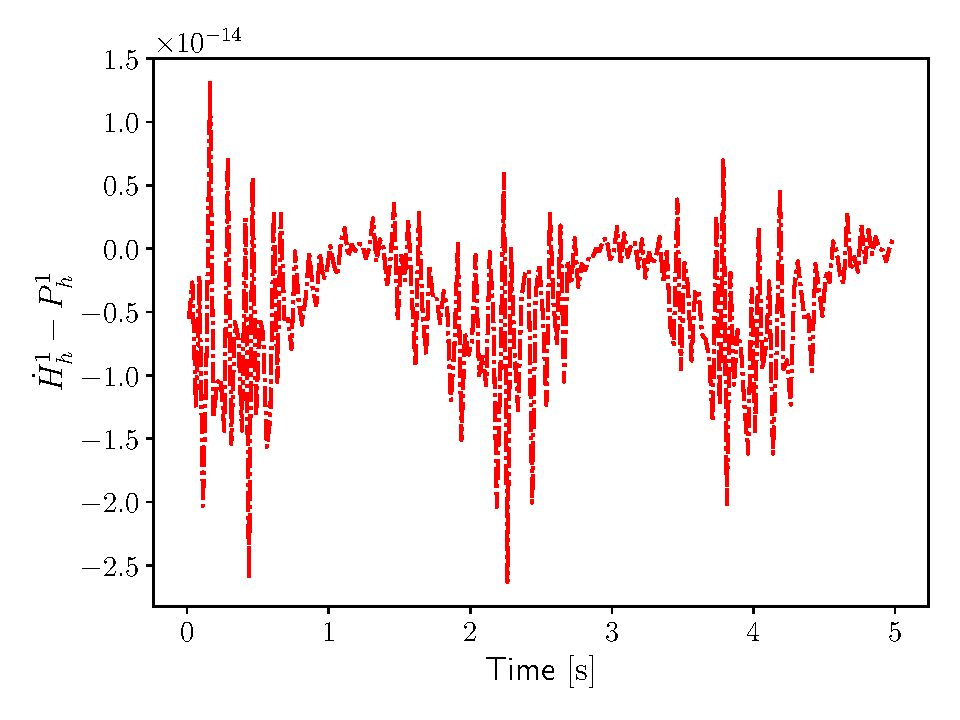
\includegraphics[width=0.48\columnwidth]{pow_bal10_3D_DN.pdf}}%
\caption{Conservation properties given by Prop. \ref{pr:discrtime_energyrate} ($N_{\text{el}}=4,\; s=3$ and $\Delta t = \frac{5}{200}$)}%
\label{fig:con_Hdot_wave}%
\end{figure}

\begin{figure}[p]%
\centering
\subfloat[][Conservation of $P_h-<e_h^\partial, f_h^\partial>_{\partial M}$]{%
	\label{fig:con_P_wave}%
	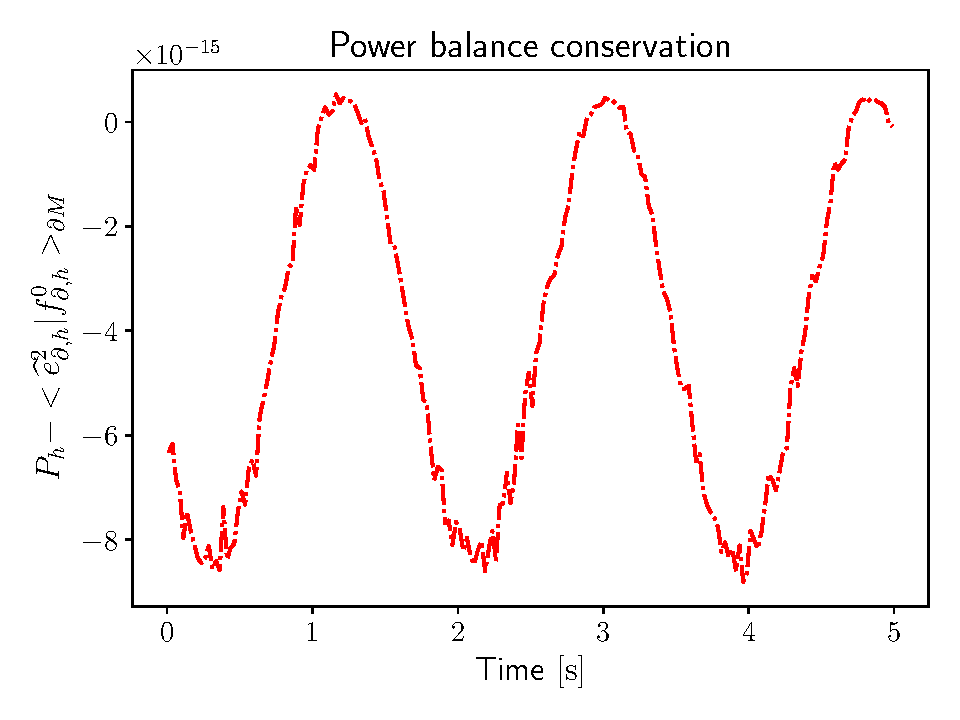
\includegraphics[width=0.48\columnwidth]{pow_bal_3D_DN.pdf}}%
\subfloat[][Error exact and interpolated boundary flow]{%
\label{fig:err_flow_wave}%
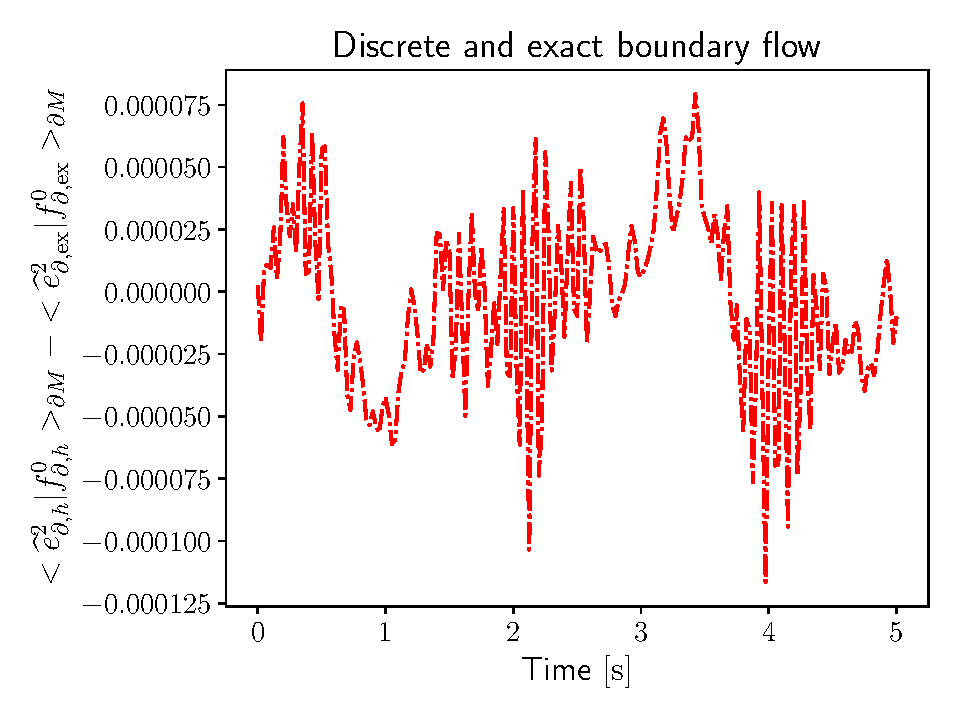
\includegraphics[width=0.48\columnwidth]{bd_flow_3D_DN.pdf}}%
\caption{discrete power balance given by Prop. \ref{pr:discrtime_Hdot} (left) and error on the power flow (right)  ($N_{\text{el}}=4,\; s=3$ and $\Delta t = \frac{5}{200}$)}%
\label{fig:con_pow_wave}%
\end{figure}

\begin{figure}[p]%
\centering
\subfloat[][Error $\dot{H}$ and interpolated boundary flow]{%
\label{fig:err_dHdt_wave}%
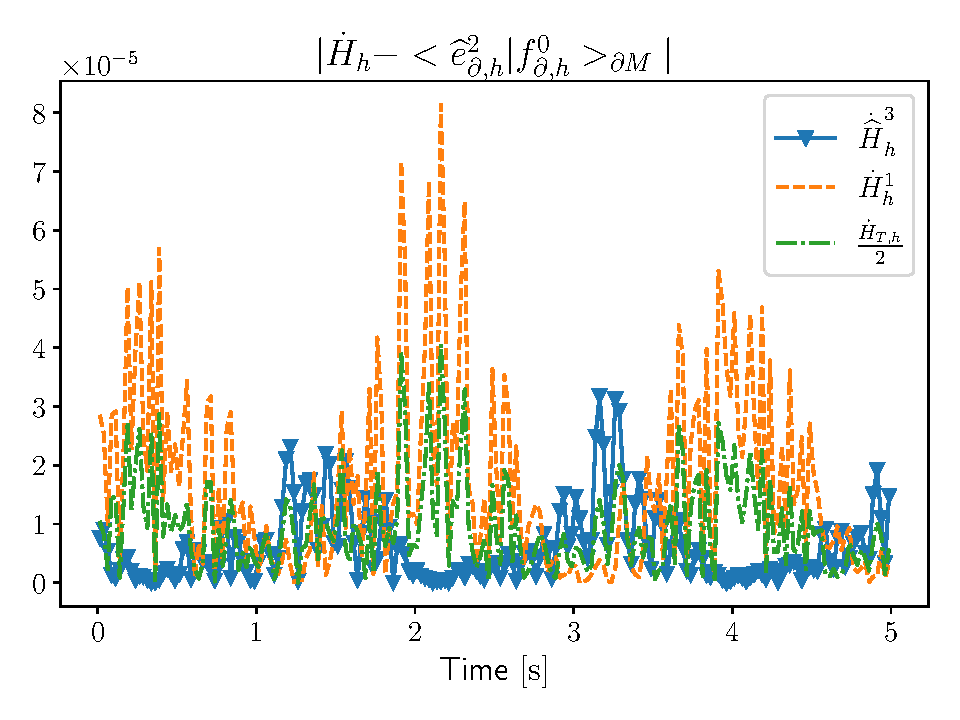
\includegraphics[width=0.48\columnwidth]{dHdt_3D_DN.pdf}}%
\subfloat[][$\Delta H_h - \Delta H_{\mathrm{ex}}$]{%
	\label{fig:deltaH_wave}%
	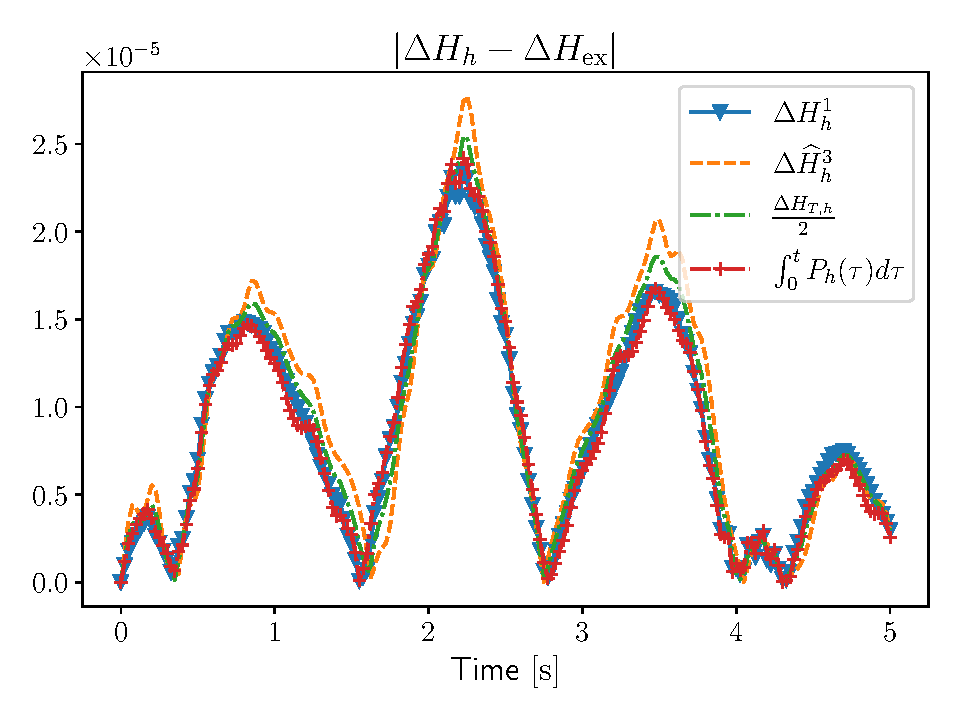
\includegraphics[width=0.48\columnwidth]{deltaH_3D_DN.pdf}}%
\caption{Energy rate and energy variation error ($N_{\text{el}}=4,\; s=3$ and $\Delta t = \frac{5}{200}$)}%
\label{fig:energy_wave}%
\end{figure}

\begin{comment}
\begin{figure}[p]%
\centering
\subfloat[][$H_h - H_{\mathrm{ex}}$]{%
	\label{fig:H}%
	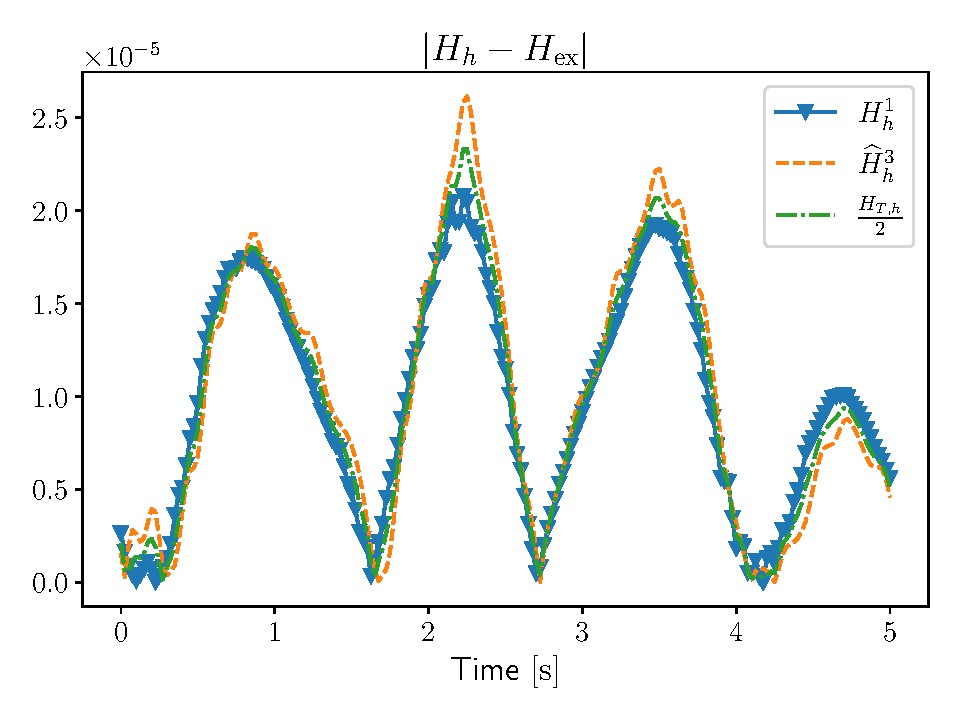
\includegraphics[width=0.48\columnwidth]{H_3D_DN.pdf}}%
\caption{Discrete and exact Hamiltonian for $\Delta t = \frac{5}{200}$}%
\label{fig:H_ex}%
\end{figure}
\end{comment}



\subsubsection{Convergence results}
In this section, the convergence rate of the different variables is verified against the analytical solution \eqref{eq:wave_exsol}.  The error is evaluated in the $L^2$ norm at the ending time. Concerning the time discretization, the total simulation time $T_{\text{end}}=1$ and the time step is taken to be $\Delta t= \frac{T_{\text{end}}}{100}$. \\

In Fig. \ref{fig:conv_var_wave} the $L^2$ error trend against the exact solution is reported for all variables. It can be noticed that the error goes as $h^s$, exception made for $p^0$ (cf. Fig. \ref{fig:err_p0}) that for $s=1, 2$ stays between $h^s$ and $h^{s+1}$. Indeed, the presence of mixed and time-varying boundary conditions leads to a lower convergence rate than the expected theoretical order of $h^{s+1}$ for homogeneous boundary conditions (see \cite{wu2021hodgewave} for the error analysis of the Hodge wave equation under one case of homogeneous conditions). The other variables exhibit the same convergence trend as predicted by the analysis in \cite{wu2021hodgewave}. The $L^2$ difference between the dual representation of the variables is reported in Fig. \ref{fig:diff_dual_wave}. The difference of the dual representation converges as $h^s$. This is in accordance with the results obtained in \cite{zhang2021mass}, where the dual field formulation is employed to solve the Navier-Stokes equations in periodic domains.
 
\begin{figure}[p]%
\centering
\subfloat[][$L^2$ error for $p^3_h$]{%
	\label{fig:err_p3}%
	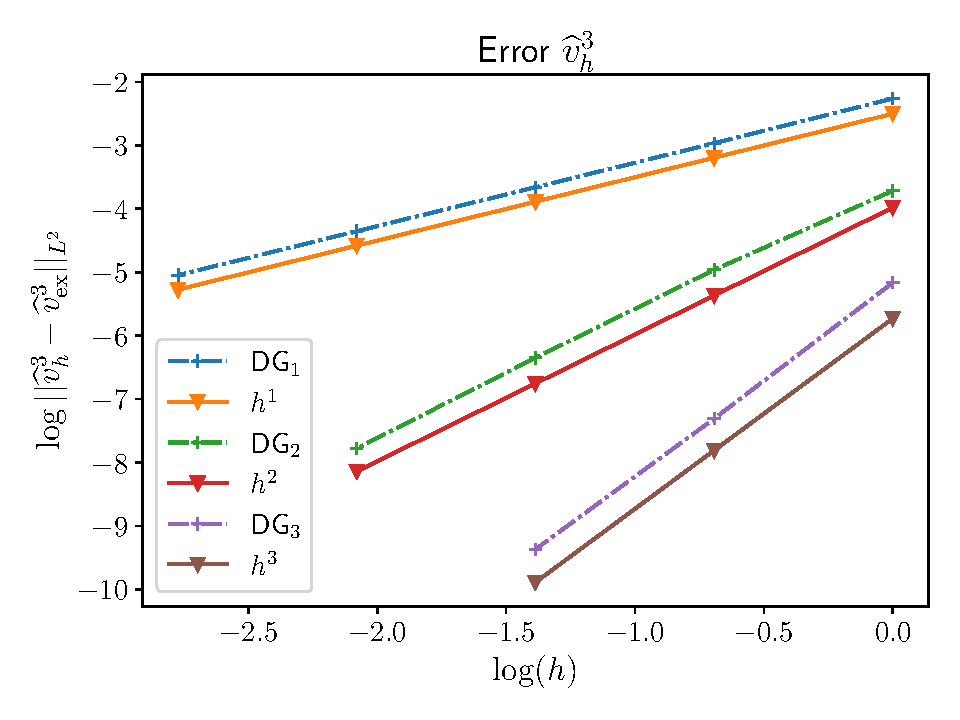
\includegraphics[width=0.48\columnwidth]{p_3_3D_DN.pdf}}%
\hspace{8pt}%
\subfloat[][$L^2$ error for $p^0_h$]{%
	\label{fig:err_p0}%
	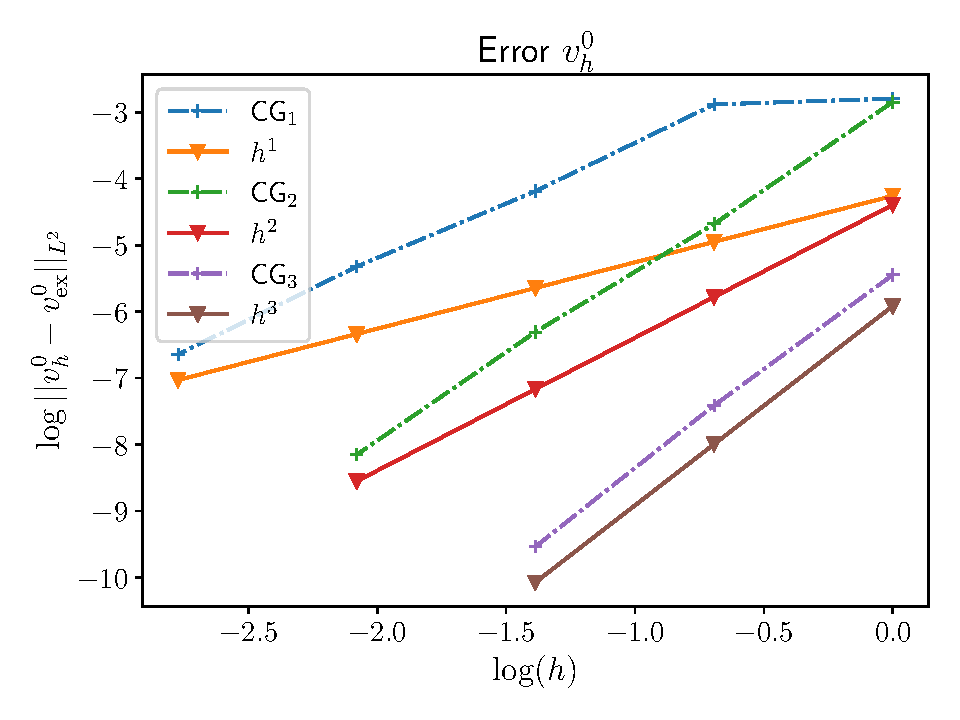
\includegraphics[width=0.48\columnwidth]{p_0_3D_DN.pdf}}%
\hspace{8pt}%
\subfloat[][$L^2$ error for $u^1_h$]{%
	\label{fig:err_u1}%
	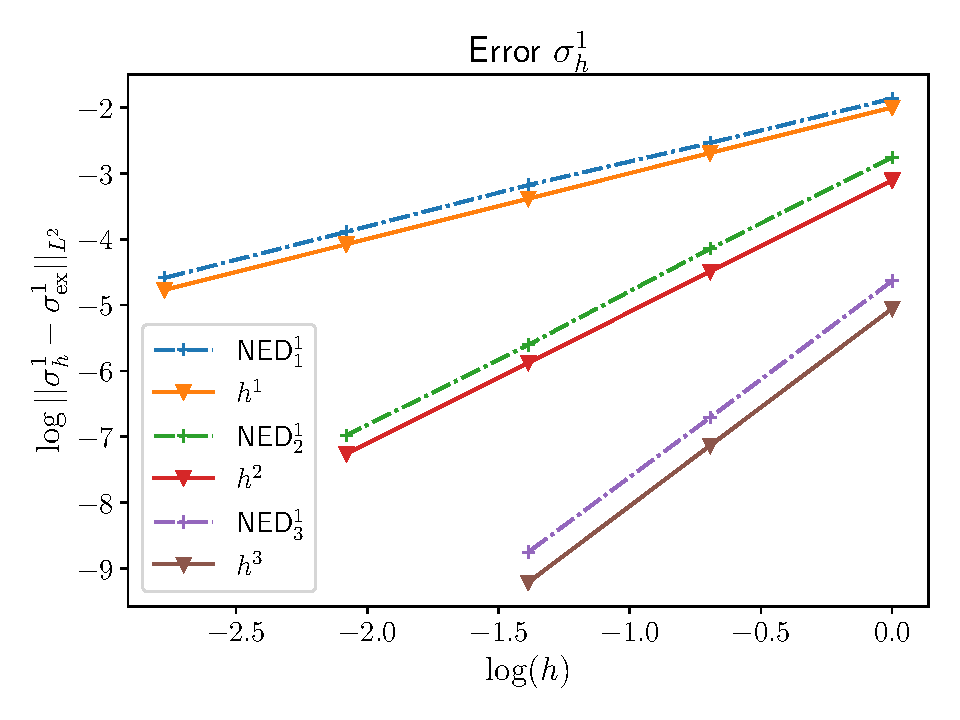
\includegraphics[width=0.48\columnwidth]{q_1_3D_DN.pdf}}
	\hspace{8pt}%
\subfloat[][$L^2$ error for $u^2_h$]{%
	\label{fig:err_u2}%
	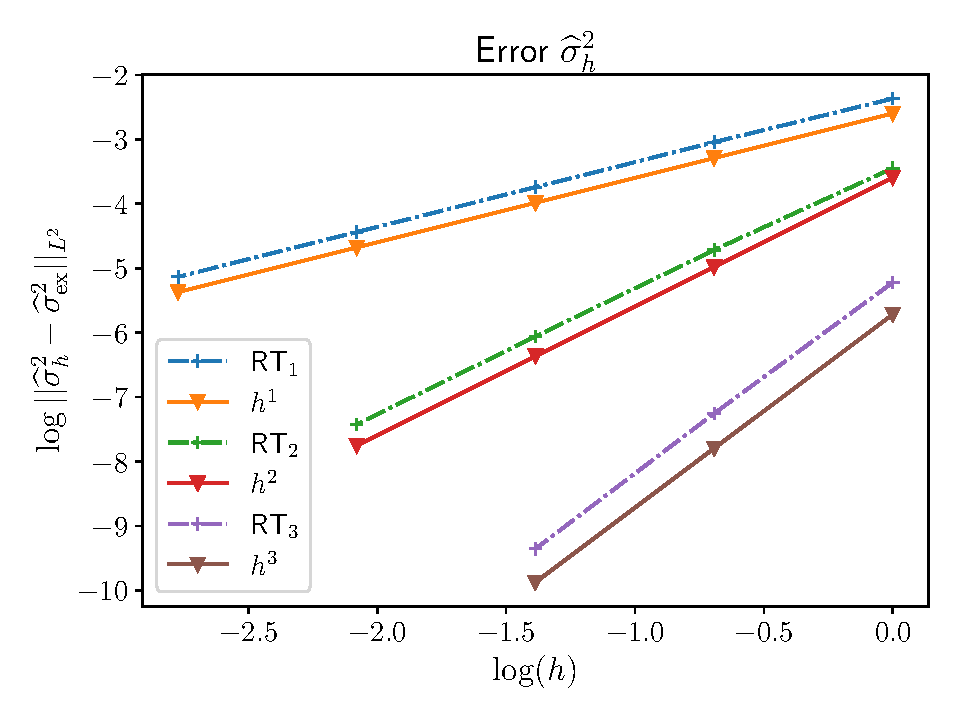
\includegraphics[width=0.48\columnwidth]{q_2_3D_DN.pdf}}
\caption{Convergence rate for the different variables in the wave equation at $T_{\text{end}}=1$ for $\Delta t = \frac{1}{100}$}%
\label{fig:conv_var_wave}%
\end{figure}

\begin{figure}[p]%
\centering
\subfloat[][$L^2$ norm of the difference $p^3_h - p^0_h$]{%
	\label{fig:diff_p30}%
	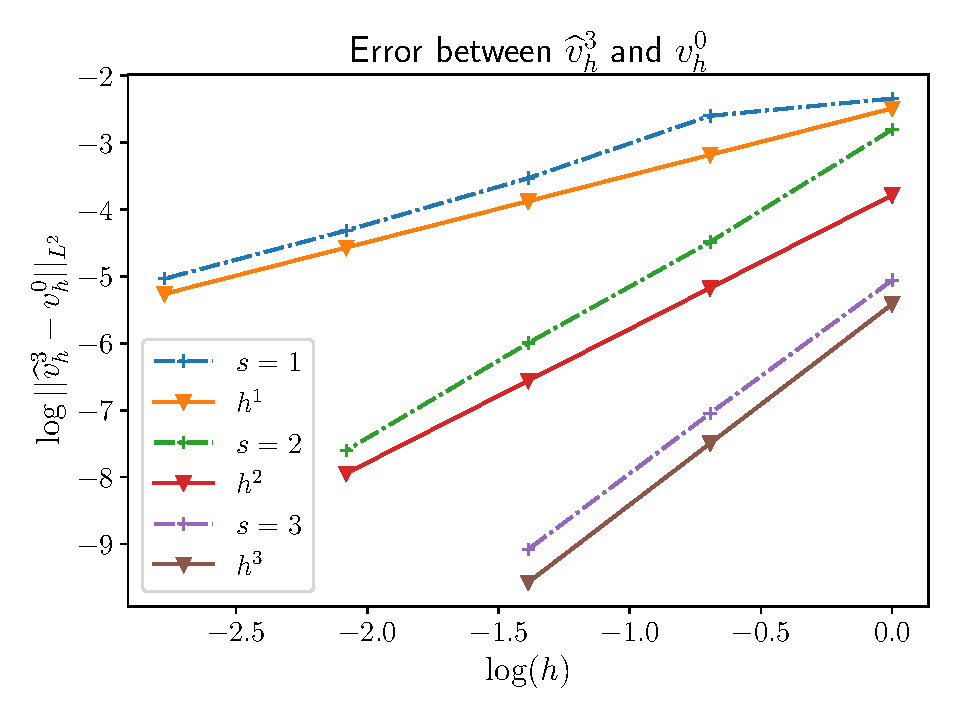
\includegraphics[width=0.48\columnwidth]{p_30_3D_DN.pdf}}%
\hspace{8pt}%
\subfloat[][$L^2$ norm of the difference $q^1_h - q^2_h$]{%
	\label{fig:diff_q12}%
	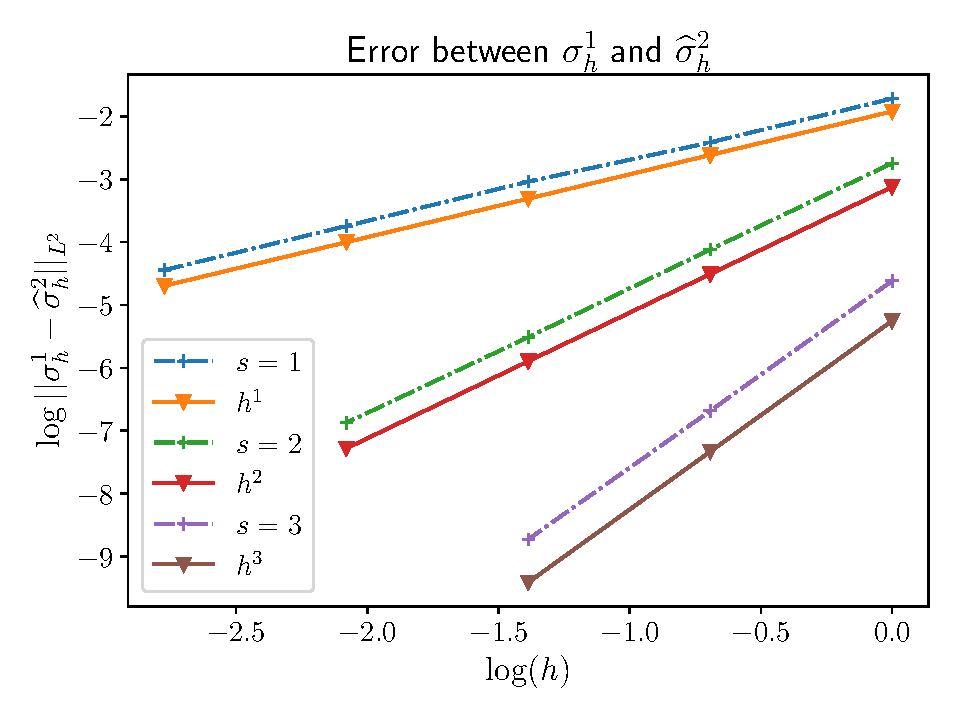
\includegraphics[width=0.48\columnwidth]{q_12_3D_DN.pdf}}%
\caption{$L^2$ difference between the dual representation of the solution for the wave equation at $T_{\text{end}}=1$ for $\Delta t = \frac{1}{100}$}%
\label{fig:diff_dual_wave}%
\end{figure}


\subsection{The Maxwell equations equation in $3D$}
The Maxwell equations corresponds to the case $p=2, \; q=2$. The energy variables correspond to the electric displacement two form $D^2 = \alpha^p$ and the magnetic field $B^2=\alpha^q$. The Hamiltonian reads
\begin{equation}
    H(D^2, B^2) = \frac{1}{2} \int_M \varepsilon^{-1} D^2 \wedge \star D^2 + \mu^{-1} B^2 \wedge \star B^2,
\end{equation}
where $\varepsilon \in \bbR$ is the electric permittivity and $\mu \in \bbR$ is the magnetic permeability. The variational derivative of the Hamiltonian are given by 
\begin{equation}
    E^1 := \delta_{D^2} H = \varepsilon^{-1} \star D^2, \qquad H^1 := \delta_{B^2} H = \mu^{-1} \star B^2.
\end{equation}
Variables $E^1, \; H^1$ are the electric field and the magnetizing field respectively. Since the reduction of the constitutive equation is such to keep only the efforts variables and their duals, the following dynamical system is obtained.
\begin{equation}\label{eq:maxwell_eq}
\begin{bmatrix}
\varepsilon & 0 \\
0 & \mu \\
\end{bmatrix}
    \begin{pmatrix}
    \partial_t E^2\\
    \partial_t H^2
    \end{pmatrix} = 
    \begin{bmatrix}
    0 & \d^1 \\
    -\d^1 & 0 \\
    \end{bmatrix}
    \begin{pmatrix}
    {E}^1\\
    {H}^1
    \end{pmatrix},
\end{equation}
where $E^2 = \star E^1, \; H^2= \star H^1$. Given the functions
\begin{equation}
    \bm{g}(x, y, z) = \begin{pmatrix}
    -\cos(x)\sin(y)\sin(z) \\
    0 \\
    \sin(x)\sin(y)\cos(z)
    \end{pmatrix}, \qquad f(t) = \frac{\sin(\omega t)}{\omega},
\end{equation}
where $\omega = \sqrt{3} c$ and $c=(\sqrt{\mu \varepsilon})^{-1}$, the system \eqref{eq:maxwell_eq} is solved by the eigenmode 
\begin{equation}\label{eq:maxwell_exsol}
\begin{aligned}
{E}^2_{\mathrm{ex}} &= \mu \star \bm{g}^\flat \diff{f}{t}, \\    
H^2_{\mathrm{ex}} &= -\d{\bm{g}^\flat} f, 
\end{aligned} \qquad
\begin{aligned}
E^1_{\mathrm{ex}} &= \mu \bm{g}^\flat \diff{f}{t}, \\    
H^1_{\mathrm{ex}} &= -\star \d{\bm{g}^\flat} f.
\end{aligned}
\end{equation}
The exact solution provides the appropriate inputs to be fed into the system
\begin{equation}
    u^p = \left. \tr E^1_{\mathrm{ex}}  \right\vert_{\Gamma_p}, \qquad u^q = \tr H^1_{\mathrm{ex}} \vert_{\Gamma_q}.
\end{equation}

The employment of the dual field discretization leads to the resolution of 4 equation is the unknowns $E^2, \; H^2$ (the dual efforts) and $E^1, \; H^1$ (the efforts). The discrete variables are represented by
\begin{itemize}
    \item Raviart-Thomas elements RT$_s$ for $E^2_h$ and $H^2_h$,
    \item Nédélec elements of the first kind NED$_s^1$ for $E^1_h$ and $H^1_h$.
\end{itemize}
For the numerical test the electric permittivity and magnetic permeability take the values
\begin{equation*}
    \mu = \frac{3}{2}, \qquad \varepsilon = 2.
\end{equation*}

\subsection{Conservation properties}

The conservation properties of the scheme are verified against the exact solution \eqref{eq:maxwell_exsol}. The test is performed using $N_{\text{el}}=4$ elements for each side of the box-shaped domain and polynomial degree $s=3$. Once again, the total simulation time $T_{\text{end}}=5$ and the time step is taken to be $\Delta t= \frac{T_{\text{end}}}{200}$. \\

An important feature of the Maxwell equations \eqref{eq:maxwell_eq} is that they verify the following constraints
\begin{equation*}
    \d^2 E^2 = 0, \qquad \d^2 H^2=0.
\end{equation*}
This result follows by taking the exterior derivative of each line of system \eqref{eq:maxwell_eq}, under the assumption that the initial conditions respect these constraints. Mixed finite element strategies, like the ones proposed in \cite{asad2019maxwell,farle2013,payen2020}, cannot satisfy both constraints as they do not employ a dual representation for each variable. Instead, the dual field formulation naturally capture this aspect as shown in Fig. \ref{fig:div_maxwell}. The energy rate conservation and discrete power balance are reported in Figs. \ref{fig:con_Hdot_maxwell} and \ref{fig:con_P_maxwell} respectively. The numerical test confirms once again the expected behaviour. The power flow error due to the polynomial interpolation is of the order of $10^{-5}$ (cf. Fig. \ref{fig:err_flow_wave}). 
For what concerns the energy behaviour, three different energies are once again considered
\begin{equation*}
\begin{aligned}
    H^{\widehat{2}2}_h&= \frac{1}{2} \int_M \varepsilon E^2_h \wedge \star E^2_h + \mu H^1_h \wedge \star H_h^1, \\
    H^{2\widehat{2}}_h&= \frac{1}{2} \int_M \varepsilon E^1_h \wedge \star E^1_h + \mu H^2_h \wedge \star H_h^2, \\
    \frac{H_T}{2} &= \frac{1}{2} \int_M \varepsilon E^1_h \wedge E^2_h + \mu H^1_h \wedge H_h^2. \\
\end{aligned}
\end{equation*}
Fig. \ref{fig:energy_maxwell} shows that the error on the energies are of the order $10^{-5}$. The dual field energy $\frac{H_T}{2}$ stays in the middle of $H^{\widehat{2}2}_h, \; H^{2\widehat{2}}_h$. The variation of energy is also computed using the power flow 
\begin{equation*}
    \Delta H = \int_0^t P_h(\tau) \d\tau, \qquad P_h = \int_M \varepsilon E^1_h \wedge \partial_t E^2_h + \mu H^1_h \wedge \partial_t H_h^2.
\end{equation*}
Indeed this variation of the energy is not the most precise (cf. Fig. \ref{fig:deltaH_maxwell}). A rigorous error analysis is needed to assess the conditions under which one of these energies perform better. 

 
\begin{figure}[tbh]%
\centering
\subfloat[][$L^2$ norm divergence of $E_h^2$]{%
	\label{fig:divE2}%
	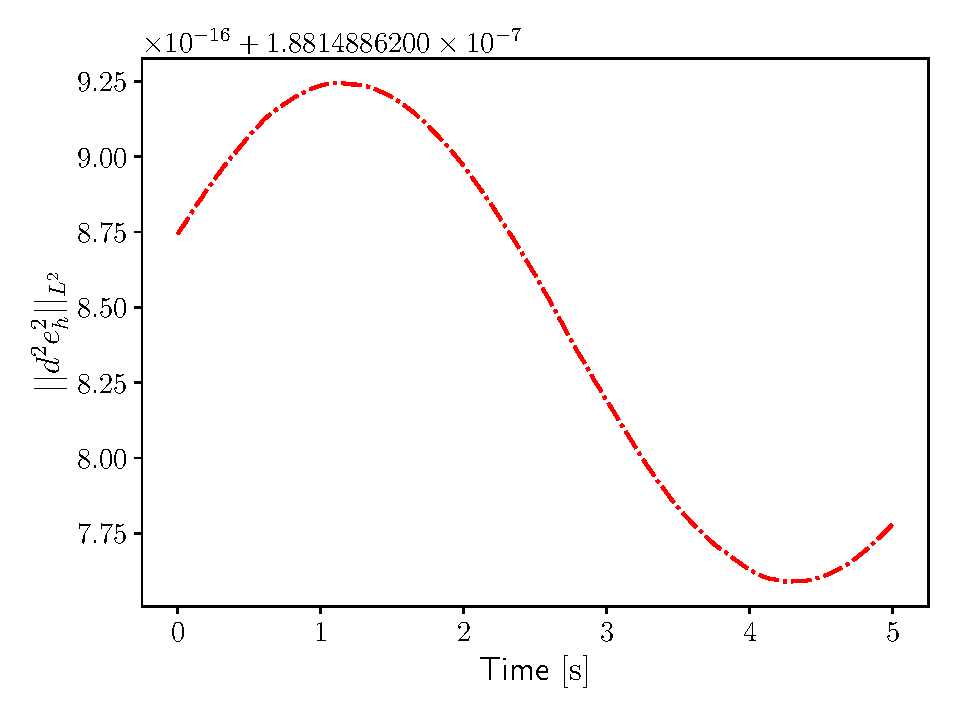
\includegraphics[width=0.48\columnwidth]{div_E2_3D_EH.pdf}}%
\hspace{8pt}%
\subfloat[][$L^2$ norm divergence of $H_h^2$]{%
	\label{fig:divH2}%
	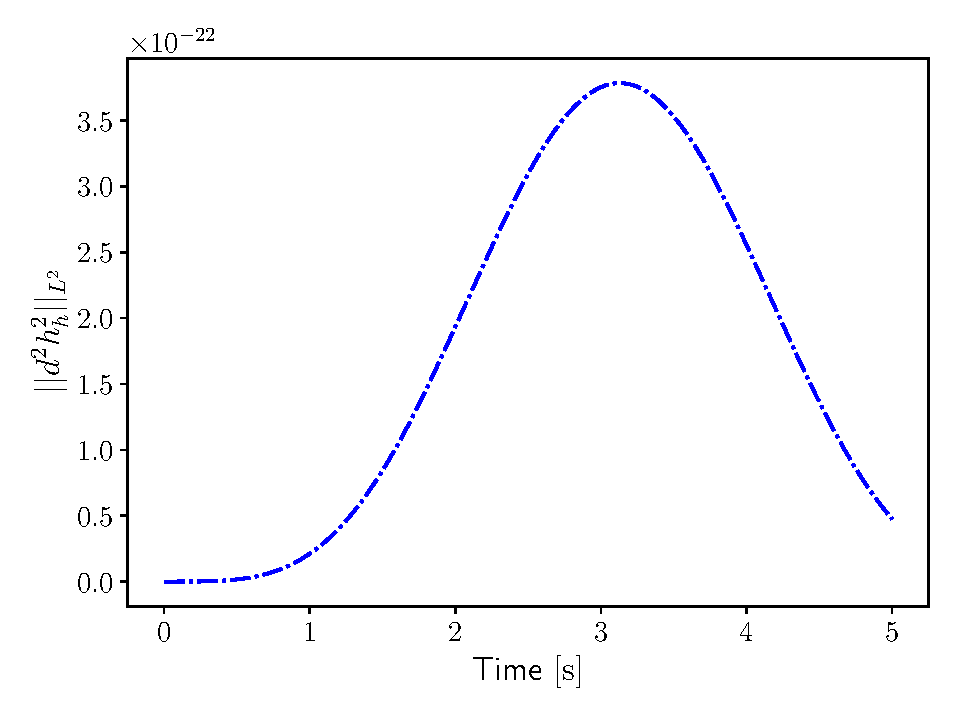
\includegraphics[width=0.48\columnwidth]{div_H2_3D_EH.pdf}}%
\caption{$L^2$ norm divergence of the two forms $E^2_h, H^2_h$}%
\label{fig:div_maxwell}%
\end{figure}

\begin{figure}[p]%
\centering
\subfloat[][Conservation law for $\dot{H}^{\widehat{2}2}_h-P^{\widehat{2}2}_h$.]{%
	\label{fig:con_H_E2H1_maxwell}%
	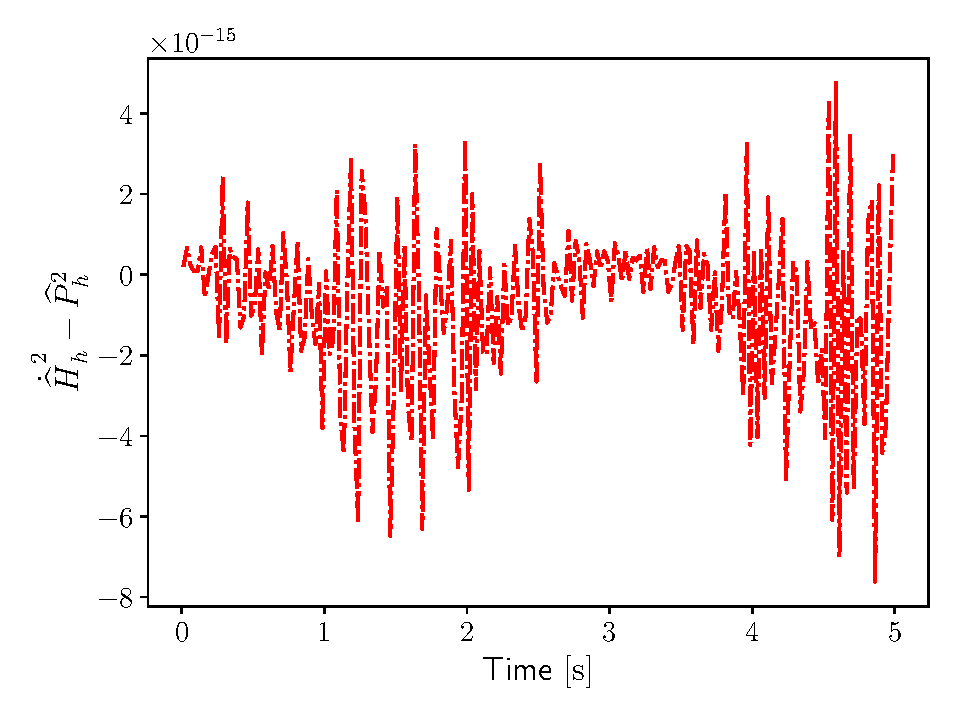
\includegraphics[width=0.48\columnwidth]{pow_balE2H1_3D_EH.pdf}}%
\hspace{8pt}%
\subfloat[][Conservation law for $\dot{H}^{2\widehat{2}}_h-P^{2\widehat{2}}_h$.]{%
	\label{fig:con_H_H2E1_maxwell}%
	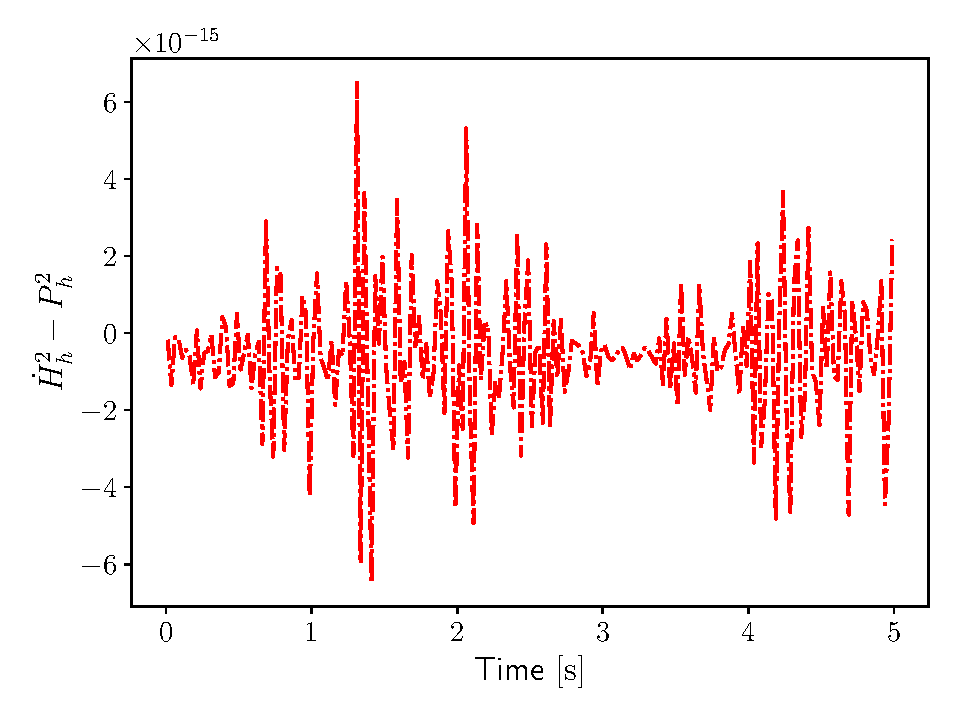
\includegraphics[width=0.48\columnwidth]{pow_balH2E1_3D_EH.pdf}}%
\caption{Conservation properties given by Prop. \ref{pr:discrtime_energyrate} ($N_{\text{el}}=4,\; s=3$ and $\Delta t = \frac{5}{200}$).}%
\label{fig:con_Hdot_maxwell}%
\end{figure}

\begin{figure}[p]%
\centering
\subfloat[][Conservation of $P_h-<e_h^\partial, f_h^\partial>_{\partial M}$.]{%
	\label{fig:con_P_maxwell}%
	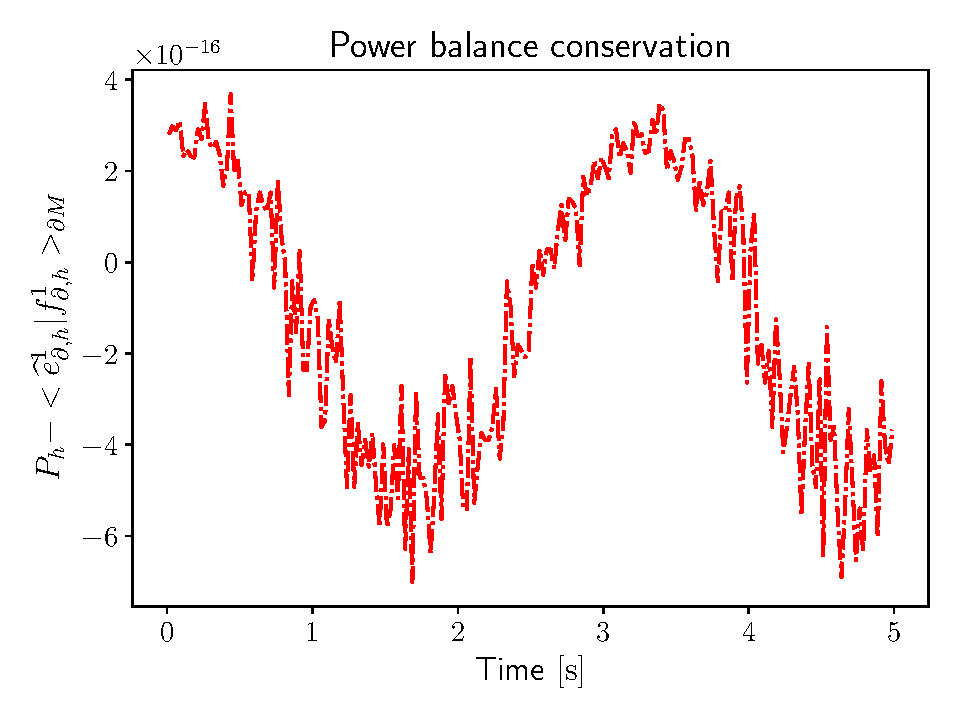
\includegraphics[width=0.48\columnwidth]{pow_bal_3D_EH.pdf}}%
\subfloat[][Error exact and interpolated boundary flow.]{%
\label{fig:err_flow_maxwell}%
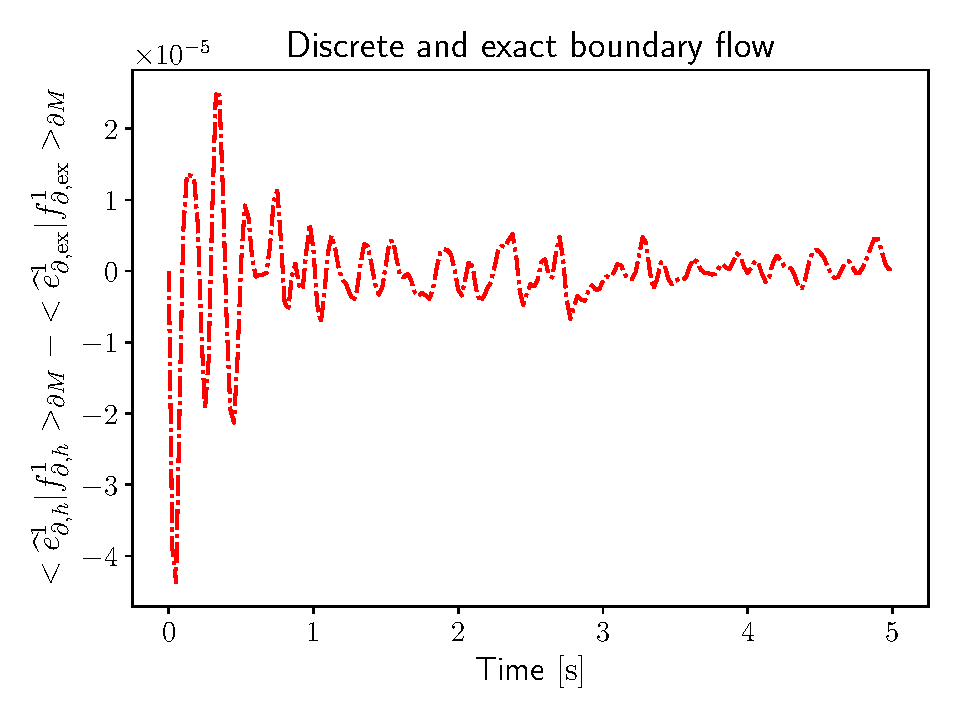
\includegraphics[width=0.48\columnwidth]{bd_flow_3D_EH.pdf}}%
\caption{Discrete power balance given by Prop. \ref{pr:discrtime_Hdot} (left) and error on the power flow (right)  ($N_{\text{el}}=4,\; s=3$ and $\Delta t = \frac{5}{200}$).}%
\label{fig:con_pow_maxwell}%
\end{figure}

\begin{figure}[p]%
\centering
\subfloat[][Error $\dot{H}$ and interpolated boundary flow]{%
\label{fig:err_dHdt_maxwell}%
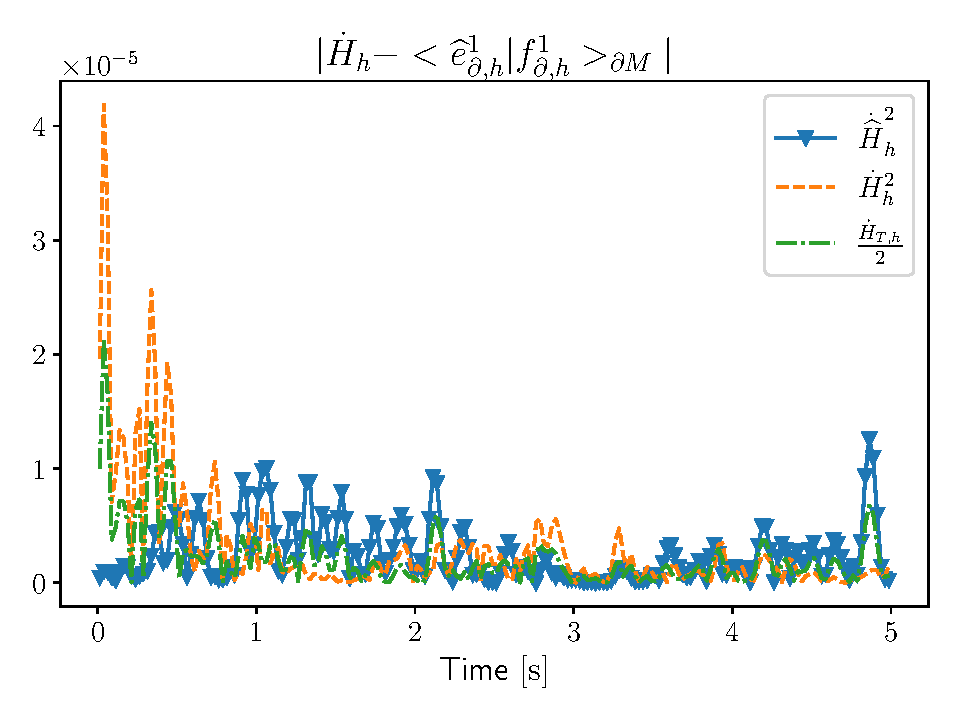
\includegraphics[width=0.48\columnwidth]{dHdt_3D_EH.pdf}}%
\subfloat[][$\Delta H_h - \Delta H_{\mathrm{ex}}$]{%
	\label{fig:deltaH_maxwell}%
	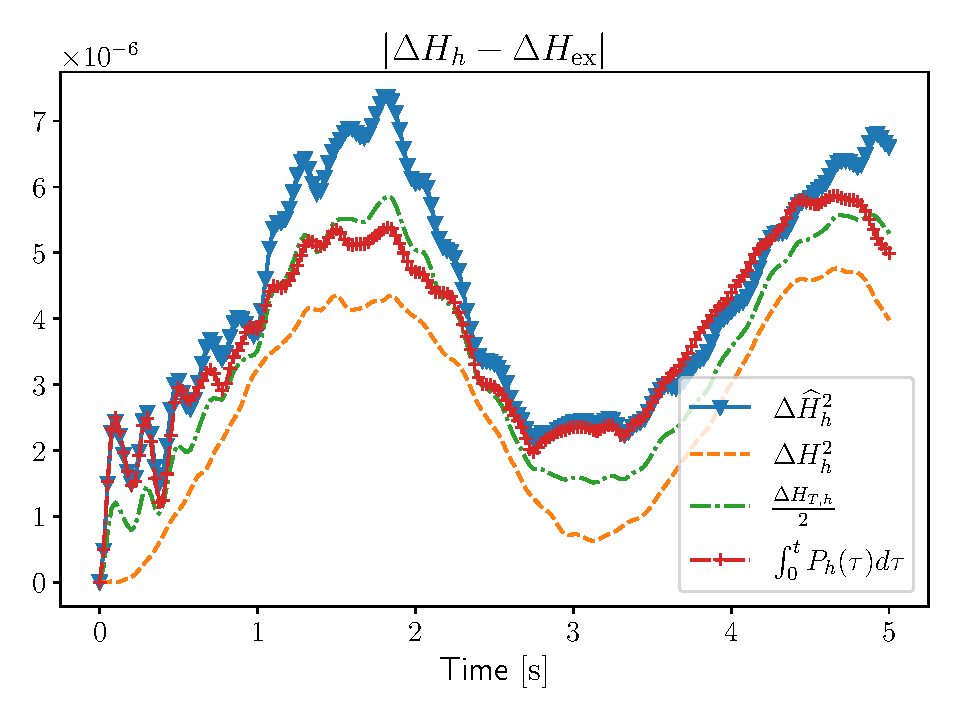
\includegraphics[width=0.48\columnwidth]{deltaH_3D_EH.pdf}}%
\caption{Energy rate and energy variation error ($N_{\text{el}}=4,\; s=3$ and $\Delta t = \frac{5}{200}$)}%
\label{fig:energy_maxwell}%
\end{figure}


\subsubsection{Convergence results}
The convergence rate of the variables with respect to the exact solution \eqref{eq:maxwell_exsol} is measured in the $L^2$ norm of the error at the final time $T_{\mathrm{end}}=1$ with time step $\Delta t = \frac{1}{100}$. \\

All variables converge with a rate given by $h^s$ (see Fig. \ref{fig:conv_var_maxwell}). However, it appears that for $s=2, 3$ variables $E^2_h$ and $H^2_h$ (Figs. \ref{fig:err_E2}, \ref{fig:err_H2}) the convergence rate is a little less than $h^s$. A rigorous error analysis is needed to gain more insight about the observed behaviour. An a priori analysis using a mixed finite element scheme can be found in \cite{asad2019maxwell}. However, therein only homogeneous and uniform boundary conditions are considered.

\begin{figure}[p]%
\centering
\subfloat[][$L^2$ error for $E^2_h$]{%
	\label{fig:err_E2}%
	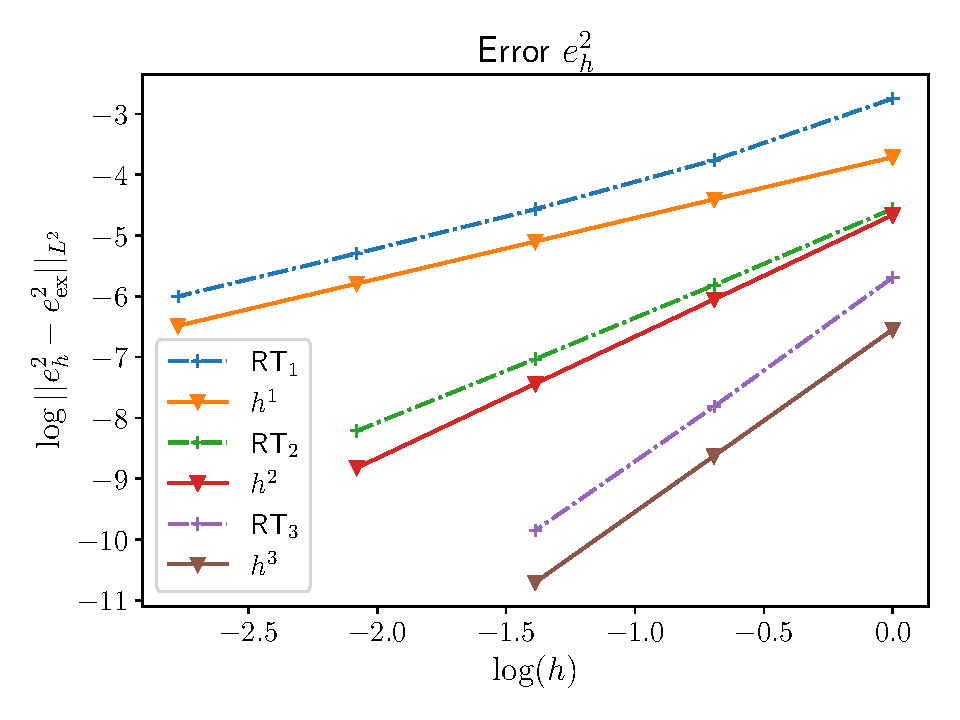
\includegraphics[width=0.48\columnwidth]{E_2_3D_EH.pdf}}%
\hspace{8pt}%
\subfloat[][$L^2$ error for $E^1_h$]{%
	\label{fig:err_E1}%
	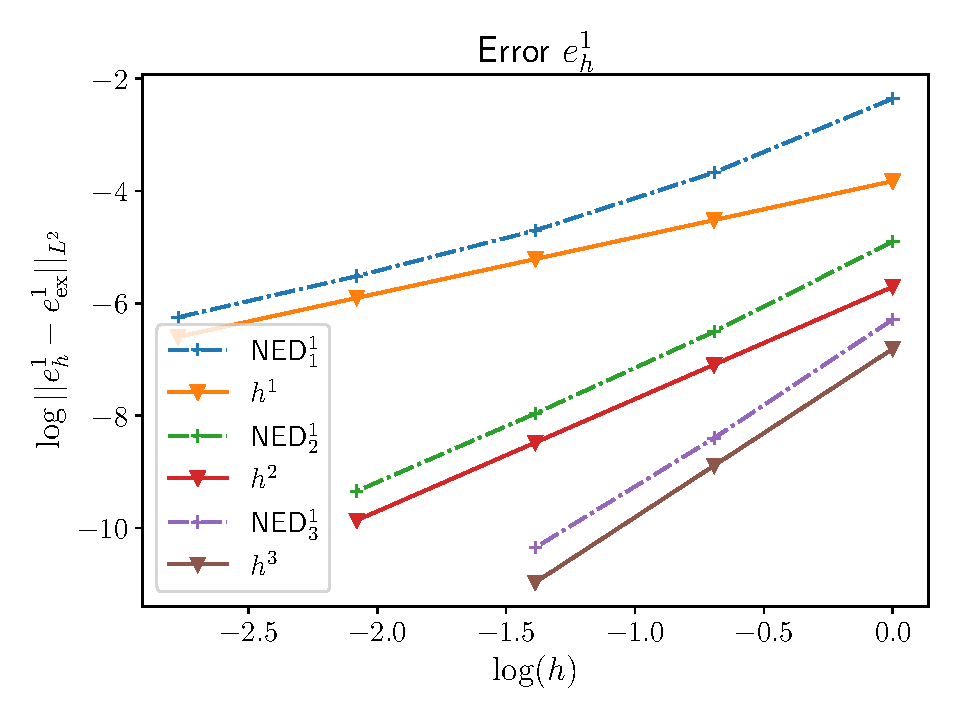
\includegraphics[width=0.48\columnwidth]{E_1_3D_EH.pdf}}%
\hspace{8pt}%
\subfloat[][$L^2$ error for $H^2_h$]{%
	\label{fig:err_H2}%
	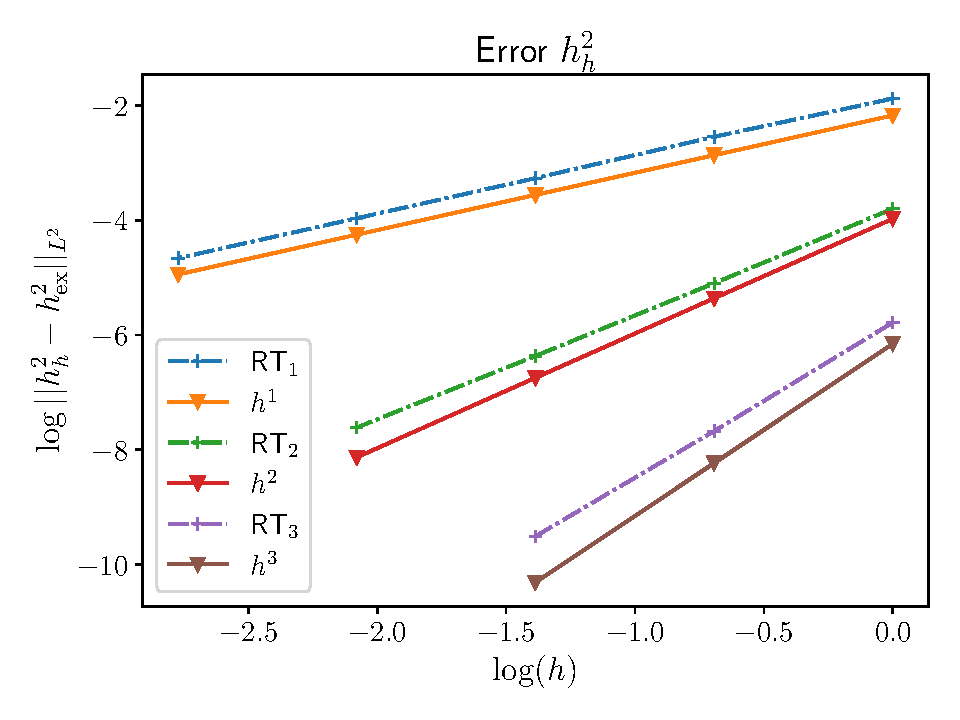
\includegraphics[width=0.48\columnwidth]{H_2_3D_EH.pdf}}
	\hspace{8pt}%
\subfloat[][$L^2$ error for $H^1_h$]{%
	\label{fig:err_H1}%
	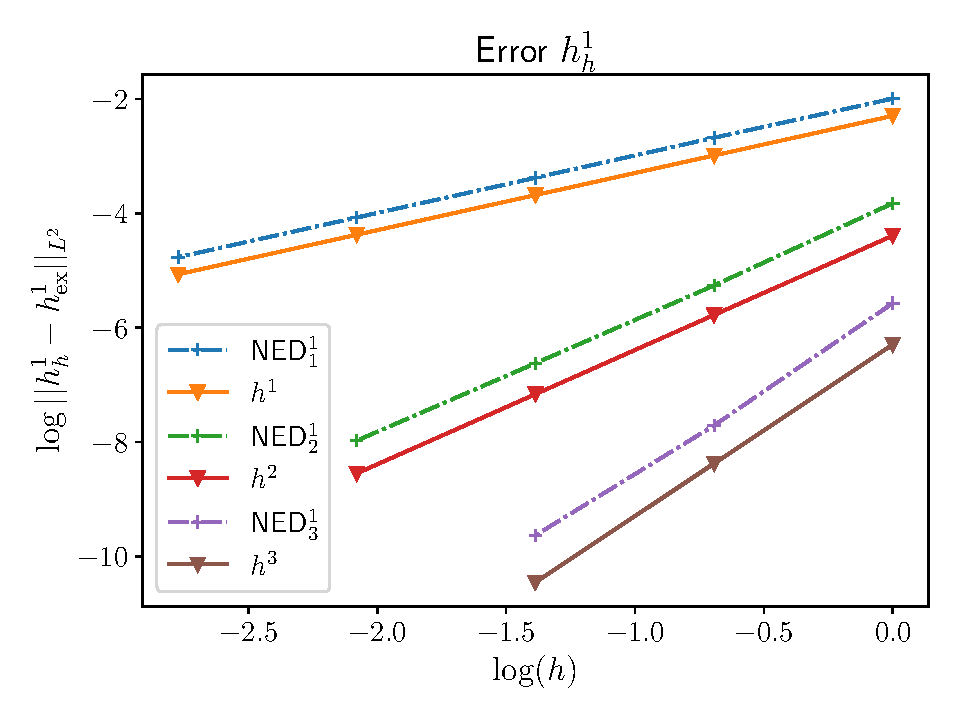
\includegraphics[width=0.48\columnwidth]{H_1_3D_EH.pdf}}
\caption{Convergence rate for the different variables in the Maxwell equations at $T_{\text{end}}=1$ for $\Delta t = \frac{1}{100}$}%
\label{fig:conv_var_maxwell}%
\end{figure}

\begin{figure}[p]%
\centering
\subfloat[][$L^2$ norm of the difference $E^1_h - E^2_h$]{%
	\label{fig:diff_E21}%
	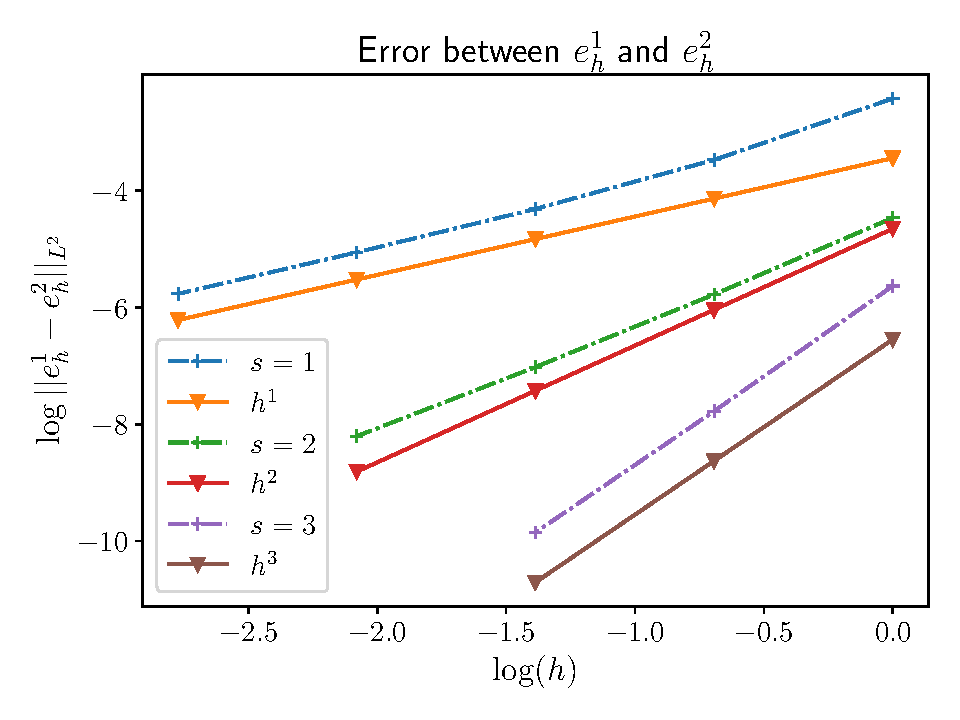
\includegraphics[width=0.48\columnwidth]{E_21_3D_EH.pdf}}%
\hspace{8pt}%
\subfloat[][$L^2$ norm of the difference $H^1_h - H^2_h$]{%
	\label{fig:diff_H21}%
	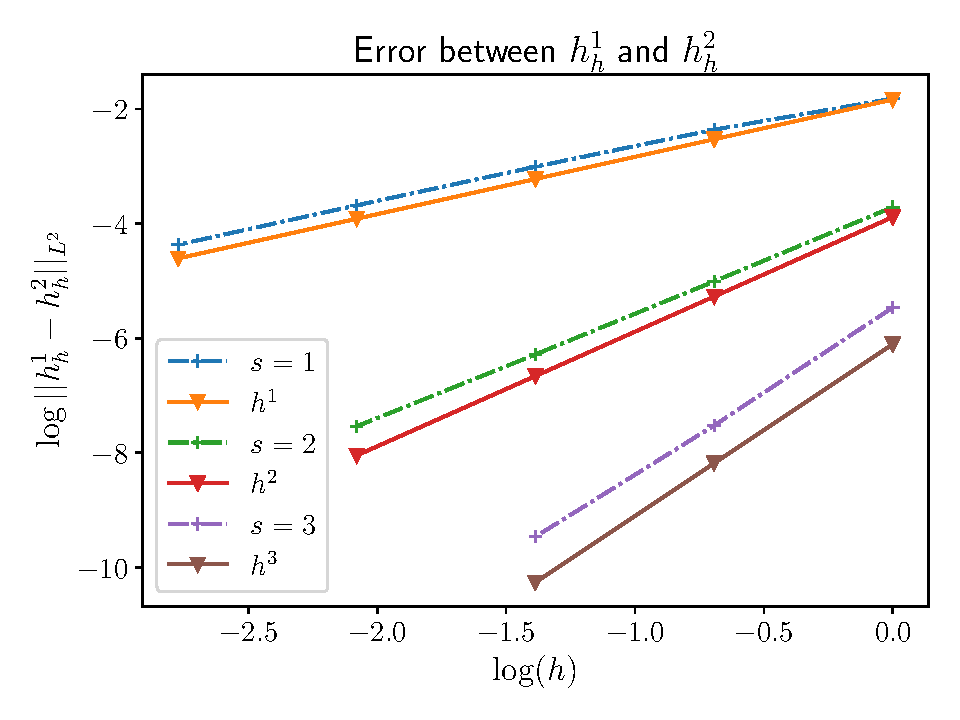
\includegraphics[width=0.48\columnwidth]{H_21_3D_EH.pdf}}%
\caption{$L^2$ difference between the dual representation of the solution for the Maxwell equations at $T_{\text{end}}=1$ for $\Delta t = \frac{1}{100}$}%
\label{fig:diff_dual_maxwell}%
\end{figure}


\section{Additional insights on the choice of the dual variables \label{sec:additionalinsights}}
Finally, we conclude by a short discussion on an alternative way of defining the diffeomorphism $\Phi$ in \eqref{eq:Phi_Diffeo} which relates the original energy variables to the dual ones and gives rise to the adjoint Stokes-Dirac structure.
Differently that presented in Sec. \ref{sec:asds}, we herewith take a definition of the Adjoint Dirac-Structure which will create an interesting symmetry between the primary system and the adjoint system. This will have as a consequence that the material operators $A^p, \; A^q$ will then appear in the adjoint Dirac-Structure. This is not useful for discretisation purposes, but is much more natural from a physical point of view, because the metrical property of space are strictly related not only to the Hodge, but to the coupling of the Hodge with the material properties.

We herewith then redefine the dual states $(\dual{\alpha}^p,\; \dual{\alpha}^q)$ to achieve a redundant representation of the state space in such a way that the dependencies on both the metric and material properties disappear. We will also redefine the dual Hamiltonian $\dual{H}(\dual{\alpha}^p,\dual{\alpha}^q)$ and we will do it here in such a way that the sum of the Hamiltonian and dual Hamiltonian is independent from the metric and material properties.
\begin{proposition}
Given any $k$-form $\alpha$ and a symmetric positive definite isomorphism $A$ between $k$ forms, if we define  $\dual{\alpha}:= \star A \alpha$, and
$\dual{C}:=(-1)^{k(n-k)}\star A^{-1} \star$ (which is symmetric positive definite), we obtain the following relations:
\begin{equation}\label{eq:EcoE}
    \inpr[M]{A \alpha}{\alpha}=\inpr[M]{\dual{\alpha}}{\dual{C}\dual{\alpha}}, \qquad \forall \alpha \in \Omega^k(M),
\end{equation}
and
\begin{equation}\label{eq:noMetric}
    \inpr[M]{A \alpha}{\alpha}+\inpr[M]{\dual{\alpha}}{\dual{C} \dual{\alpha}}
    =2\dualpr[M]{\dual{\alpha}}{\alpha}.
\end{equation}
\end{proposition}
\begin{proof}
Considering that $A$ is an isomorphism, we have that $\alpha=(-1)^{k(n-k)}A^{-1} \star \dual{\alpha}$. Since the Hodge star is an isometry, it is found
\begin{equation}
\inpr[M]{A \alpha}{\alpha} = \inpr[M]{\star A \alpha}{\star \alpha} = \inpr[M]{\dual{\alpha}}{\dual{C} \dual{\alpha}}
\end{equation}
Furthermore, one has
\begin{equation}
    \inpr[M]{\star A \alpha}{\star \alpha} = \dualpr[M]{\alpha}{\dual{\alpha}},
\end{equation}
leading to the second equation.
\end{proof}
We can therefore use the previous results by defining the following flow relations:
\[
\dual{f}^p:=\star A^p f^p
\qquad 
\dual{f}^q:=\star A^q f^q, 
\]
\noindent and the pullback of the previous map defines the effort relations:
\[
{e}^p=(-1)^{p(n-p)}\star A^p \dual{e}^p,
\qquad
{e}^q=(-1)^{q(n-q)}\star A^q \dual{e}^q.
\]
The Stokes-Dirac structure \eqref{eq:StokesDirac} is rewritten 
in terms of the co-differential map $\d^*$ defined in eq. \eqref{eq:codif}:
\begin{equation}\label{eq:AdjStokesDirac2}
    \begin{pmatrix}
    \dual{f}^{p} \\
    \dual{f}^{q} 
    \end{pmatrix} = 
    \begin{bmatrix}
        0 &  (-1)^{a_0}\
        \dual{A}^p \d^* A^q \\
        (-1)^{a_1}\ \dual{A}^q \d^* A^p & 0 \\
    \end{bmatrix}
    \begin{pmatrix}
        \dual{e}^{p}\\
        \dual{e}^{q}
    \end{pmatrix},
\end{equation}
where $\dual{A}^p = (-1)^{p(n-p)} \star A^p \star, \; \dual{A}^q = (-1)^{q(n-q)} \star A^q \star$. 
If $\dual{A}^p, \; \dual{A}^q$ are not regular enough, then they cannot be differentiate and it is necessary to invert them and bring them to the left side
\begin{equation}
\begin{bmatrix}
    \dual{C}^p & 0 \\
    0 & \dual{C}^q \\
\end{bmatrix}
    \begin{pmatrix}
     \dual{f}^{p} \\
     \dual{f}^{q} 
    \end{pmatrix} = 
    \begin{bmatrix}
        0 &  (-1)^{a_0}\
        \d^* A^q \\
        (-1)^{a_1}\  \d^* A^p & 0 \\
    \end{bmatrix}
    \begin{pmatrix}
        \dual{e}^{p}\\
        \dual{e}^{q}
    \end{pmatrix}.
\end{equation}
This system can be then put into weak form considering the integration by parts applied to the codifferential. This formulation corresponds to the dual variable elimination (cf. Remark \ref{rmk:dualelimination}) as $\dual{\alpha}^p, \; \dual{\alpha}^q$ correspond to the efforts ${e}^p, \; {e}^q$ (modulo a $\pm$ sign) and $\dual{e}^p, \; \dual{e}^q$ correspond to $\alpha^p, \; \alpha^q$. Relation \eqref{eq:EcoE}  directly gives the representation which will can be used to define the Hamiltonian of the adjoint system which then represents what in physical system theory is called the co-energy
\begin{equation}
\dual{H}(\dual{\alpha}^p(\xi, t), \dual{\alpha}^q(\xi, t))  = \int_M \frac{1}{2} \dual{C}^p \dual{\alpha}^p \wedge \star \dual{\alpha}^p + \frac{1}{2}  \dual{C}^q \dual{\alpha}^q \wedge \star  \dual{\alpha}^q.
\end{equation}
 Furthermore \eqref{eq:noMetric} immediately shows that by creating a double representation of the system with a different dual state,  the sum of the energy and co-energy, can be expressed as purely as function of the states and no extra metrical properties
\begin{equation}
   {H}({\alpha}^p(\xi, t), {\alpha}^q(\xi, t)) 
   +
   \dual{H}(\dual{\alpha}^p(\xi, t), \dual{\alpha}^q(\xi, t)) 
   = 
\int_M  
{\alpha}^p(\xi, t) \wedge 
\dual{\alpha}^p(\xi, t) 
+
{\alpha}^q(\xi, t)
\wedge
\dual{\alpha}^q(\xi, t),
\end{equation}
\noindent which shows that the sum of the energy and co-energy is independent of the metric properties expressed by $A^p$ and $A^q$ achieving a perfect symmetry. It can also be seen that in this alternative definition of the adjoint Dirac-Structure, the metric properties of space represented by the Hodge are always taken together with the physical properties of space represented by the $A$ operators as it would be expected from a physical point of view.
The insights presented above could be instructive in extending our proposed discretization scheme to nonlinear port-Hamiltonian system.

\section{Conclusion}

In this contribution, the dual field formulation is employed for the systematic discretization of linear port-Hamiltonian systems under generic boundary conditions. The proposed methodology is entirely based on the Finite Element Exterior calculus framework. The dual field formulation solves the problems associated with the construction of a discrete Hodge operator (that typically requires dual topological meshes to preserve its isomorphic character) by relying on the adjoint system. The employment of the adjoint system introduces the boundary conditions explicitly by means of the integration by part formula. This leads to two decoupled mixed discretizations that, once solved, allow retrieving a discrete power balance, regardless of the underlying boundary conditions. This guarantees that the proposed discretization method gives rise to a Dirac structure. This is of crucial importance for multiphysics applications, as well as the design of model-based control laws. \\


This methodology opens the door to a number of interesting developments. As argued in \cite{zhang2021mass}, the employment of dual representations for the unknowns provides useful indicators for adaptive meshing, as one can use the norm of the difference between dual variables as an a posteriori estimator. Furthermore, by using a time staggered discretization as in \cite{zhang2021mass} the boundary conditions could be imposed in a completely weak manner (cf. Sec. \ref{subsection:weak_bcs}). This would allow the construction of an explicit state-space model, thus avoiding the complications associated with differential algebraic systems. An interesting aspect concerns the usage of algebraic dual polynomials (proposed in \cite{jain2021algdual}) so that dual solutions can be represented in a pair of algebraically dual polynomial spaces.\\

The dual field formulation has been successfully employed to tackle the rotational term of the Navier-Stokes equations in a linear manner, leading to a computationally efficient scheme that conserves mass, energy and helicity. For this reason, we expect a non linear extension of this method to be feasible and competitive with respect to state of the art solutions. An interesting development concerns the extension of the proposed methodology to Elasticity problems. These problems require a non trivial extension of the canonical Stokes-Dirac structure, that is based on the de Rham complex, as the differential operators included in the underlying complex, the Elasticity complex, are not topological but metrical.


\section*{Funding}

This work was supported by the PortWings project funded by the European Research Council [Grant Agreement No. 787675]

\bibliography{biblio}


\appendix

\section{On higher order forms}\label{app:ho_feec}
The general construction of higher order finite element differential forms is here reported. The discussion follows \cite{wu2021hodgewave}. \\


Denote $\mathcal{P}_s(\bbR^n)$ as the space of polynomials of degree at most $s$ on an $n$-dimensional Euclidian space, and $\mathcal{H}_s(\bbR^n)$ as the space of homogeneous polynomial functions of degree $s$. Homogeneous polynomials are polynomials for which the sum of the exponents of each summing term has the same value $s$ resulting in a homogeneous function of degree $s$.

Spaces of $s$-th order polynomial differential $k-$forms, indicated as $\mathcal{P}_s\Omega^k(\bbR^n)$, and their homogeneous subclass, indicated as $\mathcal{H}_s \Omega^k(\bbR^n)$, can be defined by using the corresponding polynomials as the coefficients. Given a point $\xi \in \bbR^n$, one can treat $\xi$ as a vector in the tangential space $T_\xi\bbR^n$, and define the Koszul operator $\kappa : \Omega^k (\bbR^n) \rightarrow \Omega^{k - 1} (\bbR^n)$ 
\begin{equation}
    (\kappa\omega)_\xi(v_1, v_2, . . . , v_{k - 1}) = \omega_\xi(\xi, v_1, v_2, \dots, v_{k - 1}).
\end{equation}
The Koszul operator $\kappa$ satisfies \cite[Th. 3.1.]{arnold2006acta}
$$\kappa\d + \d\kappa = (k + s)\mathrm{Id}.$$
By means of the Koszul operator, the space of homogeneous polynomial $\mathcal{H}_s\Omega^k(\bbR^n)$, is written as the direct sum
\begin{equation}
    \mathcal{H}_s\Omega^k(\bbR^n) = \kappa \mathcal{H}_{s - 1}\Omega^{k+1}(\bbR^n) \oplus \d\mathcal{H}_{s+1}\Omega^{k - 1}(\bbR^n).
\end{equation}

Given this decomposition, the trimmed space of polynomial $k$-form is defined as
\begin{equation}
    \mathcal{P}^-_s\Omega^k(\bbR^n)  = \mathcal{P}_{s - 1}\Omega^k(\bbR^n) + \kappa \mathcal{H}_{s - 1}\Omega^{k+1}(\bbR^n).
\end{equation}
The spaces of $k$-forms on the computational mesh $\mathcal{P}_s\Omega^k(\mathcal{T}_h)$ (resp. $\mathcal{P}^-_s\Omega^k(\mathcal{T}_h)$ are obtained by restricting the forms $\mathcal{P}_s\Omega^k(\bbR^n)$ (resp. $\mathcal{P}_s^-\Omega^k(\bbR^n)$), to the elements $T$ ($n$-simplexes) of the computational mesh~$\mathcal{T}_h$. The following finite element spaces are then obtained
\begin{equation}
\begin{aligned}
    \mathcal{P}_s\Omega^k(\mathcal{T}_h) &= \{\omega \in H\Omega^k(M) |\quad \omega|_T \in \mathcal{P}_s\Omega^k(T) \quad \forall T \in \mathcal{T}_h\}, \\
\mathcal{P}_s^-\Omega^k(\mathcal{T}_h) &= \{\omega \in H\Omega^k(M) |\quad \omega|_T \in \mathcal{P}_s^-\Omega^k(T) \quad \forall T \in \mathcal{T}_h\}.
\end{aligned}
\end{equation}
The Whitney forms correspond to the case $\mathcal{P}_1^-\Omega^k(\mathcal{T}_h) = \mathcal{P}_0\Omega^k(\mathcal{T}_h) + \kappa \mathcal{P}_0\Omega^k(\mathcal{T}_h)$. The degrees of freedom for the space $\mathcal{P}_s\Omega^k(T)$ are given by
\begin{equation}\label{eq:dof_P}
    \omega \in \mathcal{P}_s\Omega^k(T) \rightarrow \int_{\sigma_j} (\tr_{\sigma_j} \omega) \wedge \mu, \qquad \mu \in \mathcal{P}^-_{s+k-j}\Omega^{j-k}(\sigma_j), \quad \sigma_j \in \Delta_j(\mathcal{T}_h), \quad j \ge k.
\end{equation}
For the space $\mathcal{P}_s^-\Omega^k(T)$ the degrees of freedom are obtained via
\begin{equation}\label{eq:dof_P-}
    \omega \in \mathcal{P}_s^-\Omega^k(T) \rightarrow \int_{\sigma_j} (\tr_{\sigma_j} \omega) \wedge \mu, \qquad \mu \in \mathcal{P}_{s+k-j-1}\Omega^{j-k}(\sigma_J), \quad \sigma_j \in \Delta_j(\mathcal{T}_h), \quad j \ge k.
\end{equation}
These polynomial spaces form a subcomplex of the de Rham complex.
\begin{theorem}{\cite[Lemma 3.8]{arnold2006acta}}\label{th:fe_subcomplex}
The complexes $(\mathcal{P}_s\Omega^k(\mathcal{T}_h), \d), \; (\mathcal{P}_s^-\Omega^k(\mathcal{T}_h), \d)$ forms a subcomplex of $(H\Omega^k(M), \d)$
\begin{equation*}
    \d\mathcal{P}_s\Omega^k(\mathcal{T}_h) \subset \mathcal{P}_{s-1}\Omega^{k+1}(\mathcal{T}_h), \qquad \d\mathcal{P}^-_s\Omega^k(\mathcal{T}_h) \subset \mathcal{P}^-_s\Omega^{k+1}(\mathcal{T}_h),
\end{equation*}
or graphically
\begin{equation*}
\begin{aligned}
    0\longrightarrow \mathcal{P}_s\Omega^0(\mathcal{T}_h) \overset{\d}{\longrightarrow} \mathcal{P}_{s - 1}\Omega^1(\mathcal{T}_h) \overset{\d}{\longrightarrow} \dots \overset{\d}{\longrightarrow} \mathcal{P}_{s - n}\Omega^n(\mathcal{T}_h) \longrightarrow 0.\\
    0 \longrightarrow \mathcal{P}^-_s \Omega^0(\mathcal{T}_h) \overset{\d}{\longrightarrow} \mathcal{P}^-_s \Omega^1(\mathcal{T}_h) \overset{\d}{\longrightarrow} \dots
\overset{\d}{\longrightarrow} \mathcal{P}^-_s \Omega^n(\mathcal{T}_h) \longrightarrow 0.
\end{aligned}
\end{equation*}
\end{theorem}
One fundamental property of the finite element differential forms is the fact that their projector commute with the exterior derivative (this property is also called cochain property). 
\begin{theorem}\cite[Th. 5.2.]{arnold2006acta}
Denoting by  $\Pi_{s, h}^{k}$ (resp. $\Pi_{s, h}^{-, k}$) the projector onto the space $\mathcal{P}_s\Omega^k(\mathcal{T}_h)$ (resp. $\mathcal{P}_s^-\Omega^k(\mathcal{T}_h)$), one has 
\begin{equation}
    \d \Pi_{s, h}^{k} \omega^k = \Pi_{s-1, h}^{k+1} \d \omega^k, \qquad \d \Pi_{s, k}^{-, k} \omega^k = \Pi_{s, h}^{-, k+1} \d \omega^k, \quad \omega^k \in \Omega^k(M).
\end{equation}

\begin{figure}[h]
\centering
\begin{tikzcd}
H\Omega^k(M) \arrow[r, "\d^k"] \arrow[d, "\Pi_{s, h}^{k}"]
& H\Omega^{k+1}(M) \arrow[d, "\Pi_{s-1, h}^{k+1}"] \\
\mathcal{P}_s\Omega^k(\mathcal{T}_h) \arrow[r, "\d^k"]
& \mathcal{P}_s\Omega^k(\mathcal{T}_h)
\end{tikzcd} \hspace{1cm}
\begin{tikzcd}
H\Omega^k(M) \arrow[r, "\d^k"] \arrow[d, "\Pi_{s, h}^{-, k}"]
& H\Omega^{k+1}(M) \arrow[d, "\Pi_{s, h}^{-, k+1}"] \\
\mathcal{P}_s^-\Omega^k(\mathcal{T}_h) \arrow[r, "\d^k"]
& \mathcal{P}_s^-\Omega^k(\mathcal{T}_h)
\end{tikzcd}  
\caption{Commuting diagrams for the finite element differential forms projectors.}
\label{fig:cd_FEDF}
\end{figure}
\end{theorem}



\section{Vector calculus and differential forms}\label{app:vec_ext}
To illustrate how existing finite element libraries can be used to implement the dual fields discretization, it is important to highlight how exterior and vector calculus are related. Let's assume that $M$ is a three dimensional Riemannian manifolds $\mathrm{dim}(M)=3$with metric $g$ and associated tangent bundle $TM$ and cotangent bundle $T^*M =\Omega^1(M)$. Denoting a generic point in the manifold as
$\xi$, using the metric tensor and the Hodge operator, vector fields can be converted into one-forms or $n-1$-forms and vice-versa.

\begin{definition}[Flat operator]
The flat isomorphism $\flat$ 
\begin{equation}
    \flat: T_\xi M \rightarrow \Omega^1_\xi(M),
\end{equation}
defined by
\begin{equation}
v^\flat(w):= g_\xi(v, w), \qquad \forall w \in T_\xi M,
\end{equation}
converts vector fields into one-forms by using the metric structure of the manifold.
\end{definition}
The inverse operator is called the sharp operator.
\begin{definition}[Sharp operator]
The sharp isomorphism $\sharp$
\begin{equation}
    \sharp: \Omega^1_\xi(M) \rightarrow T_\xi M
\end{equation}
defined by
\begin{equation}
    g_\xi(\omega^\sharp, v) := \omega(v), \qquad \forall w \in T_\xi M,
\end{equation}
converts one forms into vector fields and it is the inverse of the flat operator
\end{definition}
By combining the flat and Hodge one can convert vector fields to $n-1$ forms
\begin{equation}
\begin{aligned}
    \beta: T M &\rightarrow \Omega^{n-1}(M), \\
             v &\rightarrow  \beta(v):= \star v^\flat.
\end{aligned}
\end{equation}
The inverse operator is given by
\begin{equation}
    \beta^{-1}= (-1)^{n+1} \sharp \star.  
\end{equation}


\section{Proofs}\label{app:proofs}

\paragraph{Proof of Proposition \ref{pr:parity_a0_a1}}
A necessary and sufficient condition for two coefficients to have the same parity is that their sum is even
\begin{equation*}
    a_0 + 1 + p(n-p) \equiv 0 \mod{2}, \qquad  a_1 + 1 + r + q(n-q) \equiv 0 \mod{2}.
\end{equation*}
Considering that $p+q=n+1$, it is obtained
\begin{equation}
\begin{aligned}
    a_1 + 1 + r + q(n-q) &\equiv n +1 + p(n-p) + q(n-q) + np + pq \mod{2},\\
            &\equiv n + 1 - p - q + 2pq + np + pq, \mod{2} \\
            &\equiv p(n+q) \mod{2}, \\
            &\equiv 2pq + p(p-1) \equiv 0 \mod{2}.
\end{aligned}
\end{equation}

A similar computation then shows
\begin{equation}
    a_0 + 1 + p(n-p) \equiv 0 \mod{2}.
\end{equation}

\end{document}
